
% Predloga za pisanje zaključnih nalog, LADISK 2015-2018, pripravila Martin Česnik, Janko Slavič
% Zadnja verzija na: https://github.com/ladisk/latex-templates
\documentclass[12pt,a4paper,oneside,fleqn]{report}

%!TEX program = lualatex

% use quite a lot of packages
\usepackage[a-3u]{pdfx}
\usepackage{amsfonts,amssymb,amsmath}
\usepackage{enumerate}
\usepackage[section]{placeins}
\usepackage{float}
%\usepackage[slovene]{babel}
\usepackage[utf8]{inputenc}
\usepackage{graphicx}
\usepackage{ifthen}
\usepackage{notoccite}
\usepackage{fancyhdr}
\usepackage{epstopdf}
\usepackage{enumitem}
\usepackage{longtable}
\usepackage{hyperref}
\usepackage{ifoddpage}
\usepackage{tocloft}
\usepackage{titlesec}
\usepackage{pdfpages}
\usepackage{nameref}
\usepackage{multirow}
\usepackage{caption}
\usepackage{subcaption}
\usepackage{url}
\usepackage{icomma}
\usepackage{cite}
\usepackage{makecell}
\usepackage{colortbl}
\usepackage[numbib]{tocbibind}
\usepackage[slovene]{datetime2}
\usepackage[inner=20mm,
            outer=20mm,
            top=30mm,
            bottom=30mm]{geometry}
\usepackage{cancel}
\usepackage{graphicx}
\usepackage{pgfplots}
\usepackage{xcolor}
\usepackage[dvipsnames]{xcolor}
\usepackage{mathtools}
\usepackage{caption}
\usepackage{subcaption}
\usepackage{wrapfig,lipsum}


\titleformat{\chapter}[hang]{\normalfont\Large\bfseries}{\thechapter}{1em}{}
\titlespacing*{\chapter}{0pt}{-30pt}{10pt}
\titleformat{\section}[hang]{\normalfont\large\bfseries}{\thesection}{1em}{}

\titlespacing*{\section}{0pt}{0pt}{0pt} % Adjust the second and third arguments to control the spacing


%paragraph settings
\setlength\parindent{0pt}
\setlength{\parskip}{1.5ex plus 0.5ex minus 0.5ex}

% set equation environment indentation
\setlength{\mathindent}{0.5cm}%

% set itemize environment whitespacing and left margin
\setlist[itemize]{noitemsep,nolistsep, leftmargin=*}

% set table and figure captions
\captionsetup[table]{skip=10pt,singlelinecheck=false}
\captionsetup[figure]{justification=centering}

% set tablename to Preglednica
\AtBeginDocument{%
	\renewcommand\tablename{Table}
}

% command for multiline cell in table
\newcommand{\minitab}[2][l]{\begin{tabular}{#1}#2\end{tabular}}


% set section and tableofcontents depth
\setcounter{secnumdepth}{3}
\setcounter{tocdepth}{3}
\def\labelitemi{--}


% set fancy_nohead fancy header
\fancypagestyle{fancy_nohead}{
	\fancyfoot[RO]{\thepage}
	\fancyhead{}
	\renewcommand{\headrulewidth}{0pt}
	\chead{}
	\cfoot{}
}

% assign no_header
\assignpagestyle{\chapter}{fancy_nohead}

% table, fig and eq formatting
\renewcommand{\thetable}{\arabic{chapter}.\arabic{table}}
\renewcommand{\thefigure}{\arabic{chapter}.\arabic{figure}}
\renewcommand{\theequation}{\arabic{chapter}.\arabic{equation}}

\newcommand{\pd}{$\rightarrow$ }
\newcommand{\sln}{\textit{Source: Lecture Notes}}


% month year date format
\DTMlangsetup{showdayofmonth=false}





\begin{document}
	
	
	\pagenumbering{roman}
	% !TeX spellcheck = si_SI
%Urejanje platnic, naslovnice, UDK, povzetka in kazal
%
% PLATNICA
\hypersetup{pageanchor=false} % no page anchors for the empty-pagestyle pages
% -*- TeX:SI -*-
% Platnica
\thispagestyle{empty}
\begin{center}
\large \mbox\par\par\vspace*{-0.75cm} \textbf{FAU}
%\\ \vspace{0.2cm} \large{Fakulteta za strojništvo}
\\ \vspace*{7cm} \LARGE{\textbf{Laser Technology}}
% brez oglatih oklepajev v končni verziji -- to velja za vsa polja, kjer vnašate svoje podatke (npr. naslov, ime in priimek, datum, mentor, ....)
\\ \vspace{1cm} \normalsize
\large{Lessons}\\
\vspace{2.5cm}

\vfill
\large{Erlangen 2024}
\end{center} 
\newpage


% KAZALA
%\vspace*{0mm}
\Large\textbf{Kazalo}\normalsize
\vskip\medskipamount

% Vsebinsko kazalo
\makeatletter
\renewcommand{\tableofcontents}{\@starttoc{toc}}
\makeatother
\tableofcontents
\newpage

\vspace*{0mm}
\Large\textbf{Kazalo slik}\normalsize
\vskip\medskipamount
\addcontentsline{toc}{section}{Kazalo slik}
% Seznam slik
\makeatletter
\renewcommand{\listoffigures}{\@starttoc{lof}}
\makeatother
\renewcommand\cftfigpresnum{Slika~}
\renewcommand\cftfigaftersnum{:}

\newlength{\mylen} % a "scratch" length
\settowidth{\mylen}{\bfseries\cftfigpresnum\cftfigaftersnum} % extra space
\addtolength{\cftfignumwidth}{\mylen} % add the extra space
\setlength{\cftfigindent}{0pt}

\listoffigures


\newpage

%\vspace*{0mm}
%\Large\textbf{Kazalo preglednic}\normalsize
%\vskip\medskipamount
%\addcontentsline{toc}{section}{Kazalo preglednic}
% Seznam tabel
%\makeatletter
%\renewcommand{\listoftables}{\@starttoc{lot}}
%\makeatother

%\renewcommand\cfttabpresnum{Preglednica~}
%\renewcommand\cfttabaftersnum{:}
%\settowidth{\mylen}{\bfseries\cfttabpresnum\cfttabaftersnum} % extra space
%\addtolength{\cfttabnumwidth}{\mylen} % add the extra space
%\setlength{\cfttabindent}{0pt}

%\listoftables

%\newpage  
	\newpage
	% % !TeX spellcheck = si_SI

\vspace*{0mm}
\Large\textbf{Seznam uporabljenih simbolov}\normalsize
\vskip\medskipamount
\leaders\vrule width \textwidth\vskip0.4pt
\vskip\bigskipamount

\addcontentsline{toc}{section}{Seznam uporabljenih simbolov}
\begin{longtable}[l]{@{}p{.15\textwidth}@{}p{.15\textwidth}@{}p{.7\textwidth}@{}}
\hline
Oznaka & Enota & Pomen\\
\hline
\endfirsthead
\hline
\endhead
&&\\
$\mathbf{C}$ & N s m$^{-1}$ & globalna dušilna matrika\\



\end{longtable}
\newpage



\vspace*{0mm}
\Large\textbf{Seznam uporabljenih okrajšav}\normalsize
\vskip\medskipamount
\leaders\vrule width \textwidth\vskip0.4pt
\vskip\bigskipamount

\addcontentsline{toc}{section}{Seznam uporabljenih okrajšav}

\begin{longtable}[l]{@{}p{.2\textwidth}@{}p{.8\textwidth}@{}}
\hline
Okrajšava & Pomen\\
\hline
\endfirsthead
\hline
\endhead
&\\
CAD & računalniško podprto konstruiranje (ang. \emph{Computer Aided Design})\\
PZF & pasovno zavrnitveni filter\\
\end{longtable}

\newpage
	
	
	\fancyhf{}
	\fancyhead[RO]{\nouppercase{\leftmark}}
	
	\fancyfoot[RO]{\thepage}
	\renewcommand{\headrulewidth}{0.1mm}
	\renewcommand{\footrulewidth}{0mm}
	\cfoot{}
	\setlength{\headheight}{14.5pt}
	
	
	\pagenumbering{arabic}

        \begingroup
        \renewcommand{\cleardoublepage}{}
        \renewcommand{\clearpage}{}    
	\chapter{Electrmagnetic Waves}

\section{Light}
Light is electromagnetic radiation, figure \ref{fig:spectrum} shows the 
spectre of EM radiation. 

\begin{figure}[h!]
    \centering
    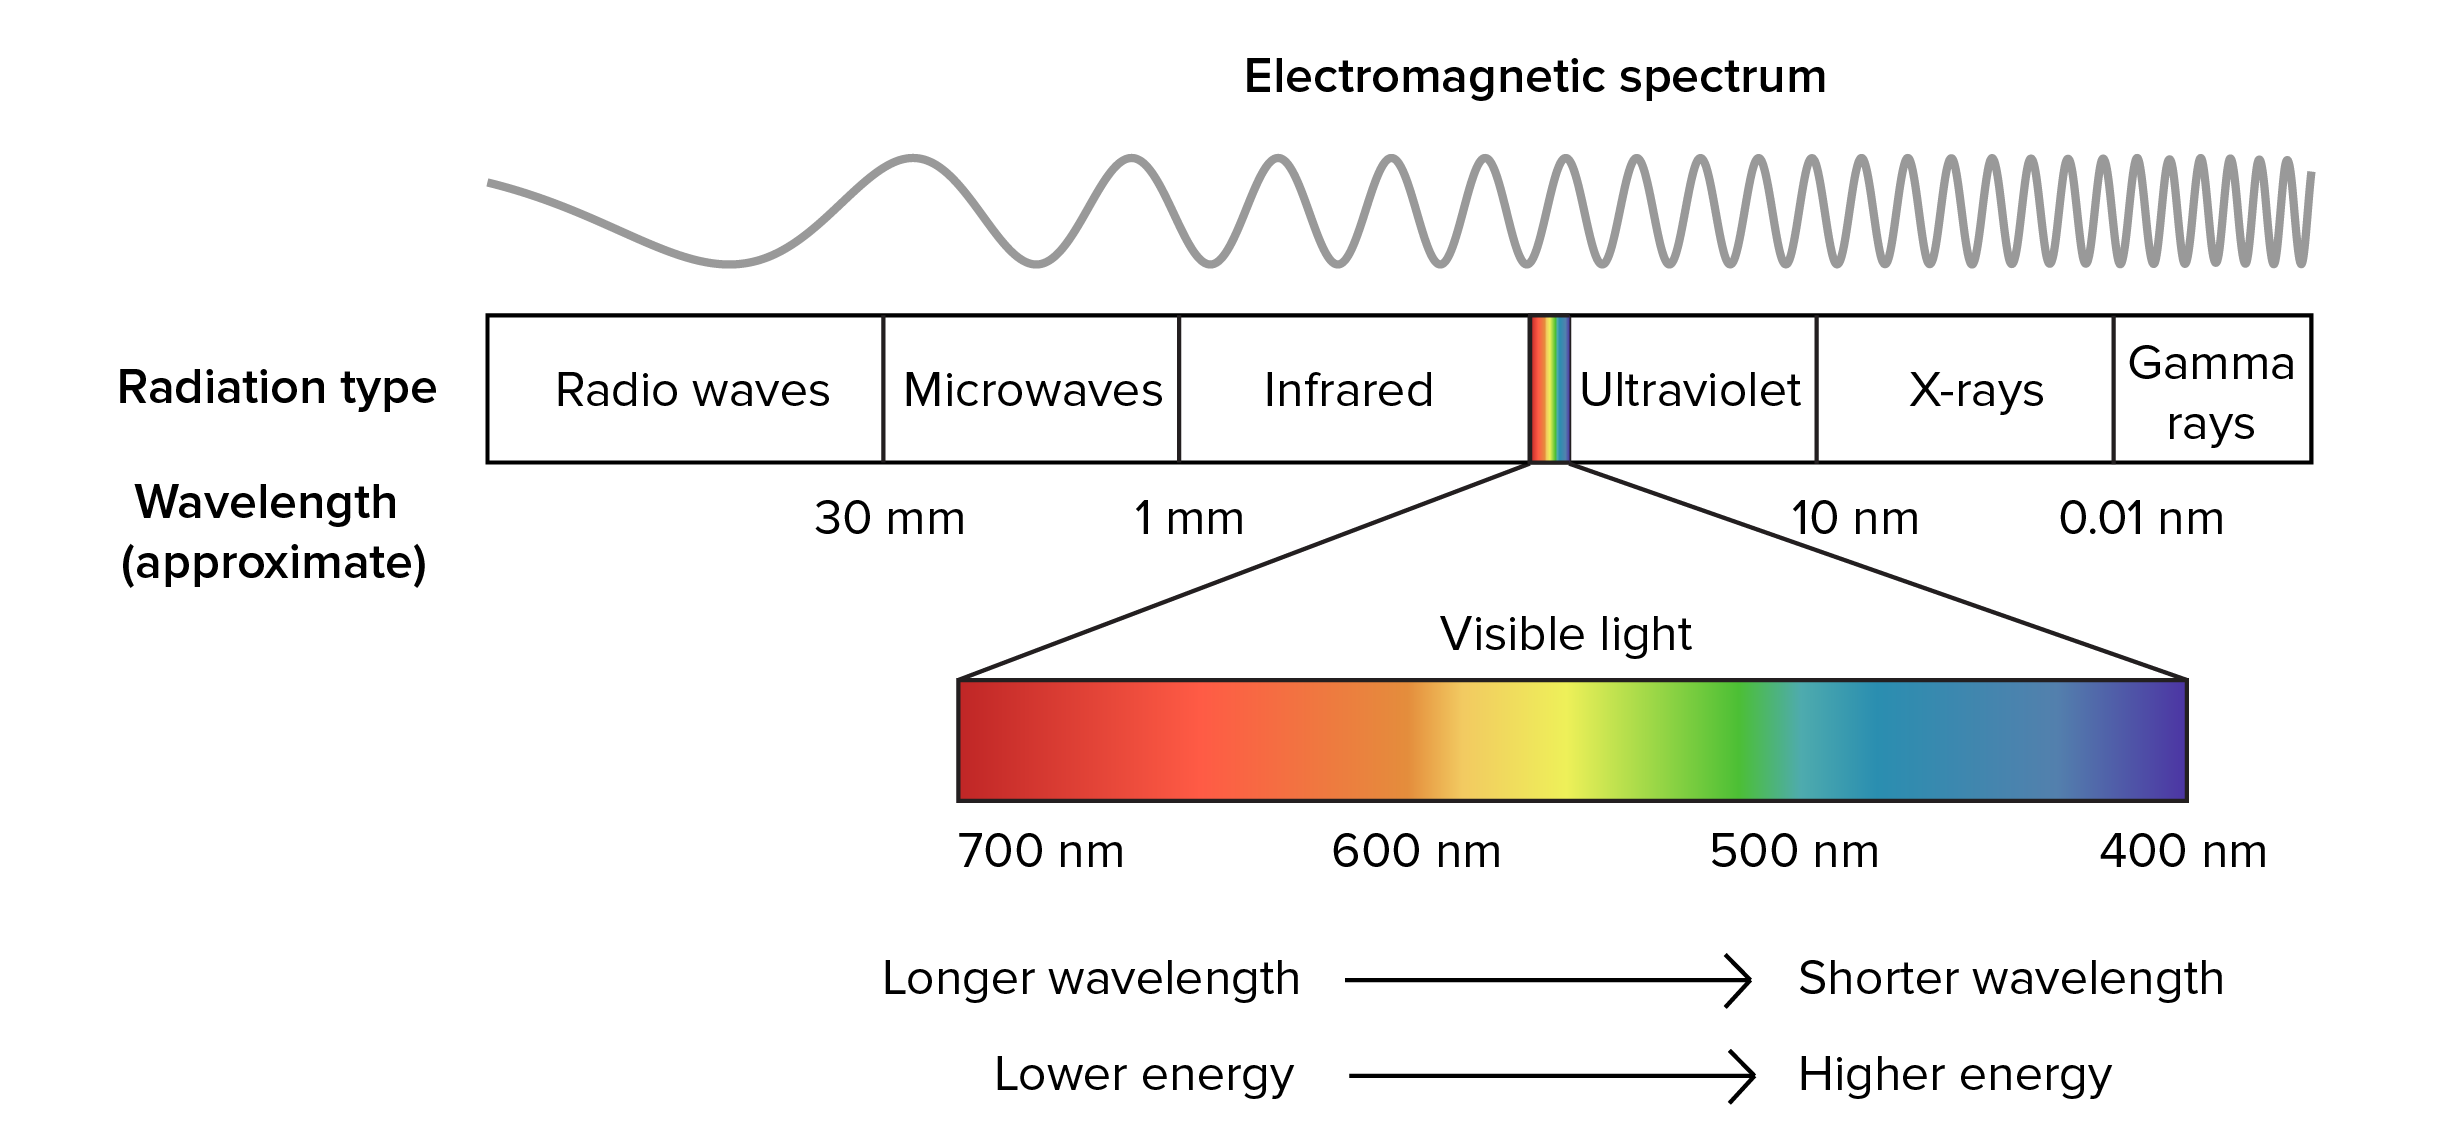
\includegraphics[width=0.5\textwidth]{slike/spectrum.png}
    \caption{Spectrum of EM}
    \label{fig:spectrum}
\end{figure}

Light of one wavelength can be described by the equation \ref{eq:light1}.
\begin{equation}
    \nu \cdot \lambda = c
    \label{eq:light1}
\end{equation}
Where $\nu$ is the frequency, $\lambda$ is the wavelength and $c$ the speed of
light. 
Speed of light is equal to $c \approx 3 \cdot 10^8 \frac{m}{s}$.

\section{Electromagnetic radiation}
An example source of EM radiation - dipole radiation -  is an oscillating electron, at a certain frequency and amplitude.
Close to the source we can describe the EM field using the \textit{Faraday's law}, equation \ref{eq:fl}.
\begin{equation}
    \nabla \times E  = - \frac{\partial B}{\partial t}
    \label{eq:fl}
\end{equation}
Where $E$ is the electric field and $B$ is the magnetic field.

Magnetic and electric fields are perpendicular to each other, as shown on figure \ref{fig:mef}.
\begin{figure}[h!]
    \centering
    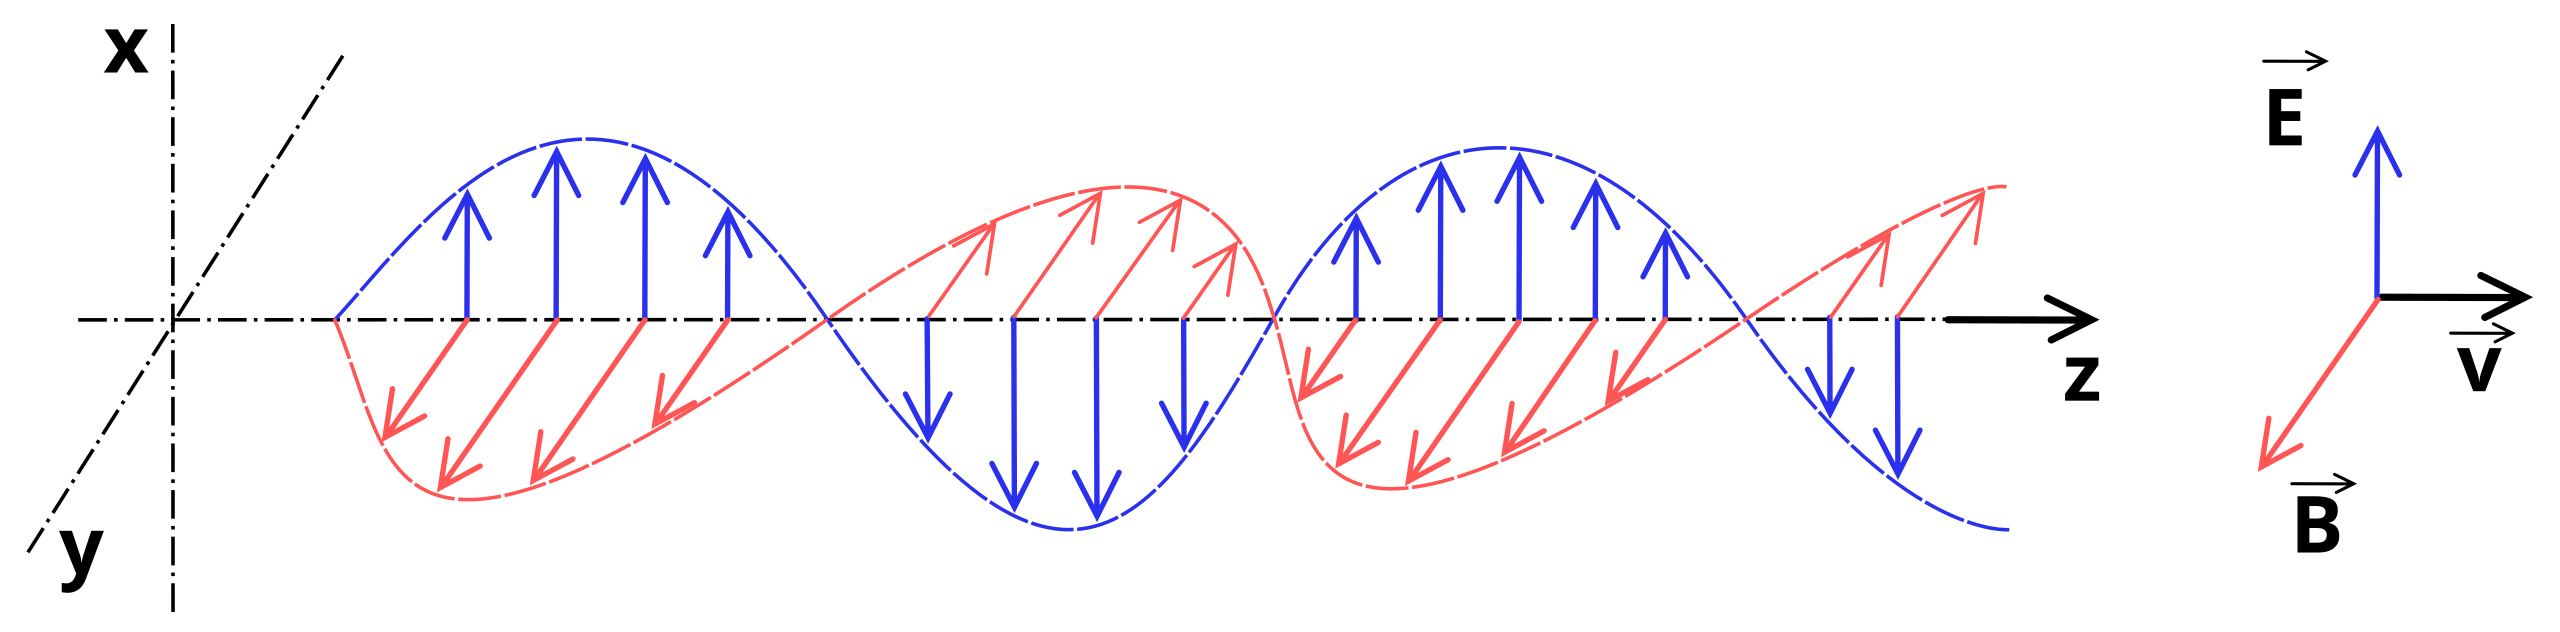
\includegraphics[width=0.5\textwidth]{slike/Onde_electromagnetique.svg.png}
    \caption{Magnetic and electric field}
    \label{fig:mef}
\end{figure}

Far from the origin, EM field is \textbf{perpendicular to propagation direction}.
Electric field and magnetic fields are synchronized and perpendicular. These two simplifications,
neglect field directions and only consider $E$ and $B$ fields along the propagation directions.
Consequences of this are:
\begin{enumerate}
    \item Loose information about 3D shape of radiation
    \item \textbf{Much simpler mathematical description}
\end{enumerate}



In summary - properties of EM-waves are:
\begin{itemize}
    \item is generated by dipole moment change
    \item electric and magnetic fields are synchronized and point towards orthogonal directions, both fields are perpendicular to the propagation direction $\rightarrow$ transverse wavelength
    \item electric and magnetic filed directions depend on the oscillation directions dependent on the oscillation orientation of the dipole $\rightarrow$ polarization
    \item oscillation frequency of the dipole determines the wavelength
\end{itemize}


\subsection{EM-wave in one dimension}
\begin{figure}[h!]
    \centering
    \includegraphics[width=0.5\textwidth]{slike/simplewave.pdf}
    \caption{Simple wave}
    \label{fig:simplewave}
\end{figure}

Where $\lambda$ is the wavelength, $A_0$ is the filed strength (amplitude), $\varphi$ is the phase delay or shift. 
From this, we can derive  wave number \ref{eq:wavenumber}:

\begin{equation}
    k = \frac{2 \pi}{\lambda}
    \label{eq:wavenumber}
\end{equation}
Angular frequency, \ref{eq:angfreq}:
\begin{equation}
    \omega = 2 \pi \nu
    \label{eq:angfreq}
\end{equation}

Using \ref{eq:angfreq} and \ref{eq:wavenumber}, we can derive \ref{eq:wave}:
\begin{equation}
    A(x,t) = A_0 cos(kx - \omega t + \varphi)
    \label{eq:wave}
\end{equation}

\subsection{EM-wave in 3D}
To describe the wave in 3D space, we can use equation \ref{eq:w3d}.
\begin{equation}
    \vec{A}(\vec{r},t) = \vec{A}_0 cos(\vec{k} \cdot \vec{r} - \omega t + \varphi)
    \label{eq:w3d}
\end{equation}

Where $A_0$ is a field vector - direction of EM-field, $\vec{r}$ is position vector in space, 
$\vec{k}$ is the wave vector - points along the propagation direction ($k_x$,$k_y$,$k_z$).
\textbf{Dot product} $\vec{k} \cdot \vec{r}$ is a constant - mathematical definition of a plane.
Figure \ref{fig:linplw} shows the linear plane wave in 3D.
%https://en.wikipedia.org/wiki/Sinusoidal_plane_wave

\begin{figure}[h!]
    \centering
    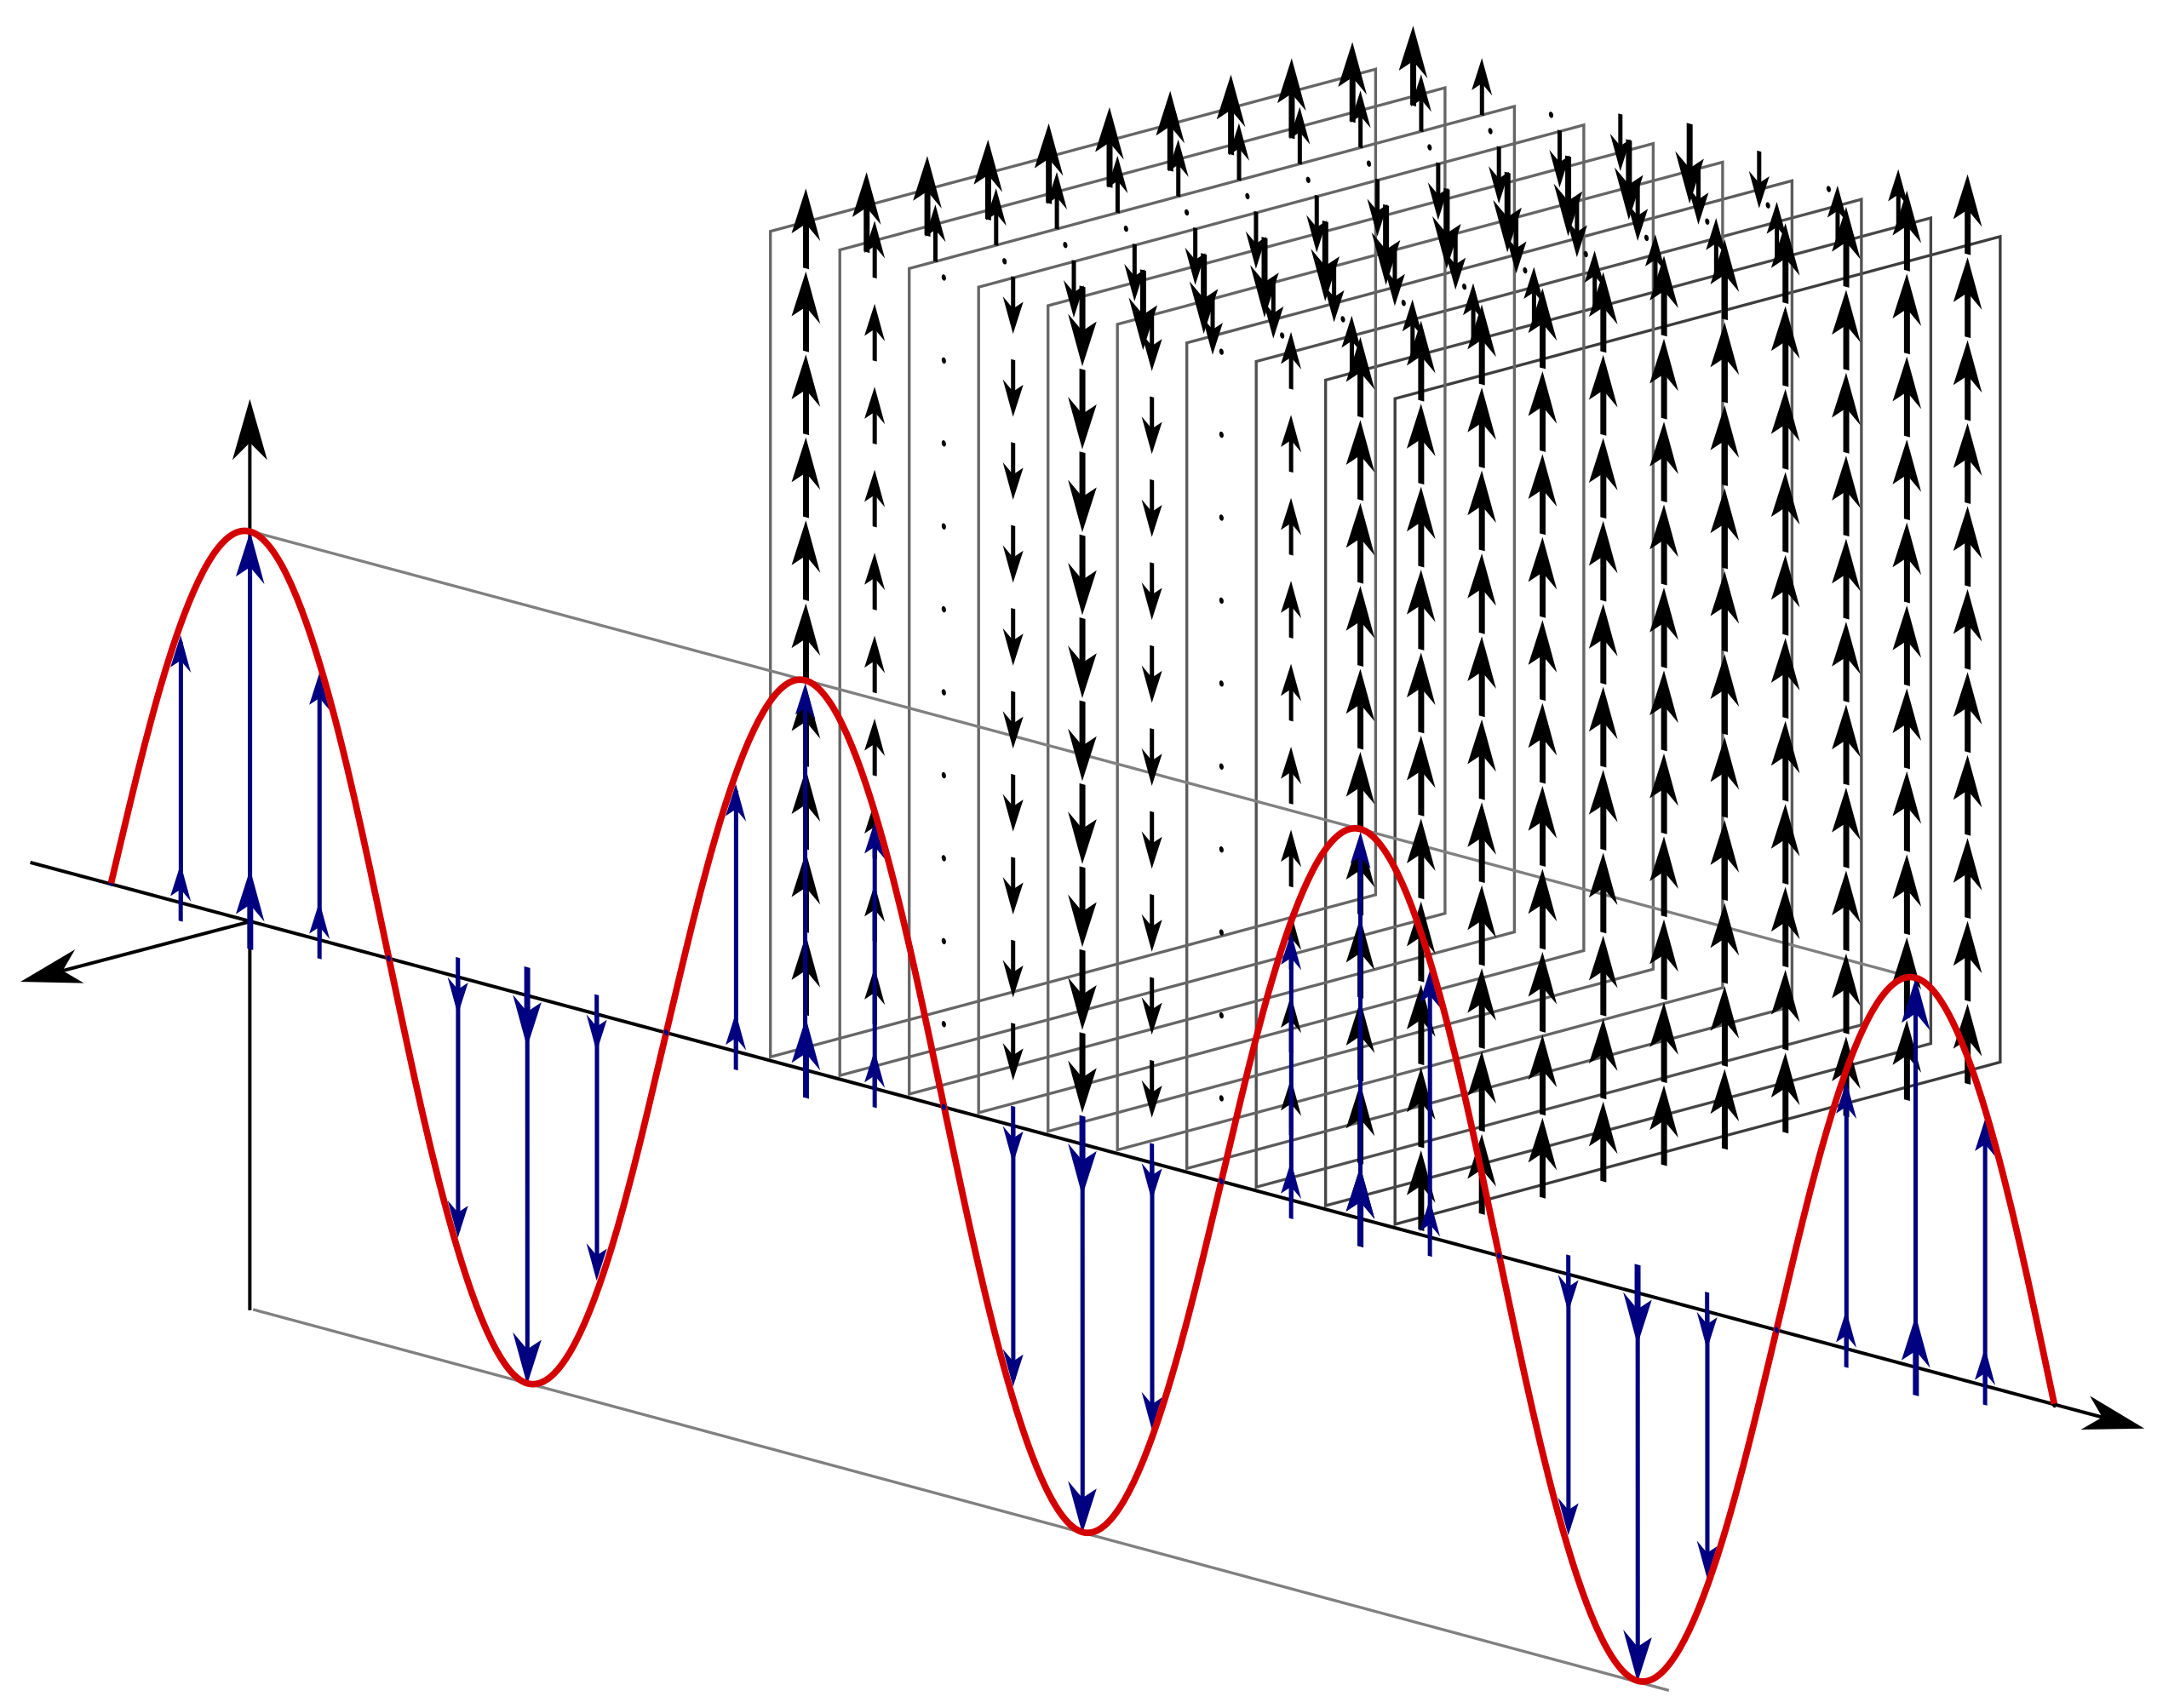
\includegraphics[width=0.4\textwidth]{slike/linplanewave.png}
    \caption{Linear plane wave}
    \label{fig:linplw}
\end{figure}

We use simplifications for describing the plane wave, its wavefronts are:
\begin{itemize}
    \item  parallel
    \item  infinite
    \item  orthogonal to propragation direction
\end{itemize}
True plane-waves do not exist, they are a convenient mathematical tool.



\section{Power and intensity}
Electric and magnetic fields store energy according to equation \ref{eq:ed}.
\begin{equation}
    u_{EM} = \frac{\varepsilon}{2} |E|^2 + \frac{1}{2\mu} |B|^2
    \label{eq:ed}
\end{equation}
Where $\varepsilon$ is permittivity of medium, $\varepsilon = \varepsilon_R \varepsilon_0$
and $\mu$ is magnetic permeability, $\mu = \mu_R \mu_0$. $\varepsilon_0$ is equal to $8.854 \cdot 10^{-12} \frac{F}{m}$.
$\mu = 1.256 \cdot 10^{-6} \frac{N}{A^{2}}$.
Figure \ref{fig:EBwave} show a diagram of a wave. At the intersections of $E$ and $B$ fields
- crossings, power is equal to zero (Green circles). This is hard to measure.
\begin{figure}[h!]
    \centering
    \includegraphics[width=0.5\textwidth]{slike/EBfield.pdf}
    \caption{E and B wave with zero crossings}
    \label{fig:EBwave}
\end{figure}

Although there is no energy in the crossings, for most practical applications
we still consider that there is \textbf{continuous energy flow}. 
We introduce \textbf{power} and \textbf{intensity}. 
Power $P = \frac{\Delta E}{\Delta t}$ and intensity is equal to $\frac{Powe}{Area}$. 
For a plane wave intensity is calculated as \ref{eq:pd}, where $n$ is the refractive index, $c$ is the speed of light and $\varepsilon_0$ is vacuum 
permittivity. 

\begin{equation}
    I = \frac{c n \varepsilon_0}{2} |E|^2
    \label{eq:pd}
\end{equation}

\subsection{Power and energy}
Power is equal to $\frac{Energy}{Time}$, unit is Watt - $W = \frac{J}{s}$.
Average power is $P = \frac{\Delta E}{\Delta t}$ and instantaneous power is $P = \frac{dE}{dt}$.
Average intensity $I = \frac{\Delta P}{\Delta A}$  and local intensity is $I = \frac{d P}{d A}$

\section{Polarization}

Polarization of an electromagnetic wave is given ny the \textbf{orientation of its electric component}. Because the magnetic field $B$ is 
negligible compared to the electric field, for polarization of light, we will \textbf{only use} $\vec{E}$.

Polarization is important due to:
\begin{itemize}
    \item Brewster angle - optical components, absorption efficiency
    \item Processing effects - laser introduced surface structures
    \item Focusing quality
    \item Birefringence effects - focus quality degradation, wavelength conversion
\end{itemize}

\subsection{Brewster angle}
Brewster angle is an angle of incidence at which light with certain polarization is 
perfectly transmitted through a transparent dielectric surface, with no reflection.
Brewster's angle is calculated as \ref{eq:brewstr}. 

\begin{equation}
    \theta_B = arctan(\frac{n_2}{n_1})
    \label{eq:brewstr}
\end{equation}

Figure \ref{fig:brewstr} show the light interacting with two different mediums, with different $n$.
\begin{figure}[h!]
    \centering
    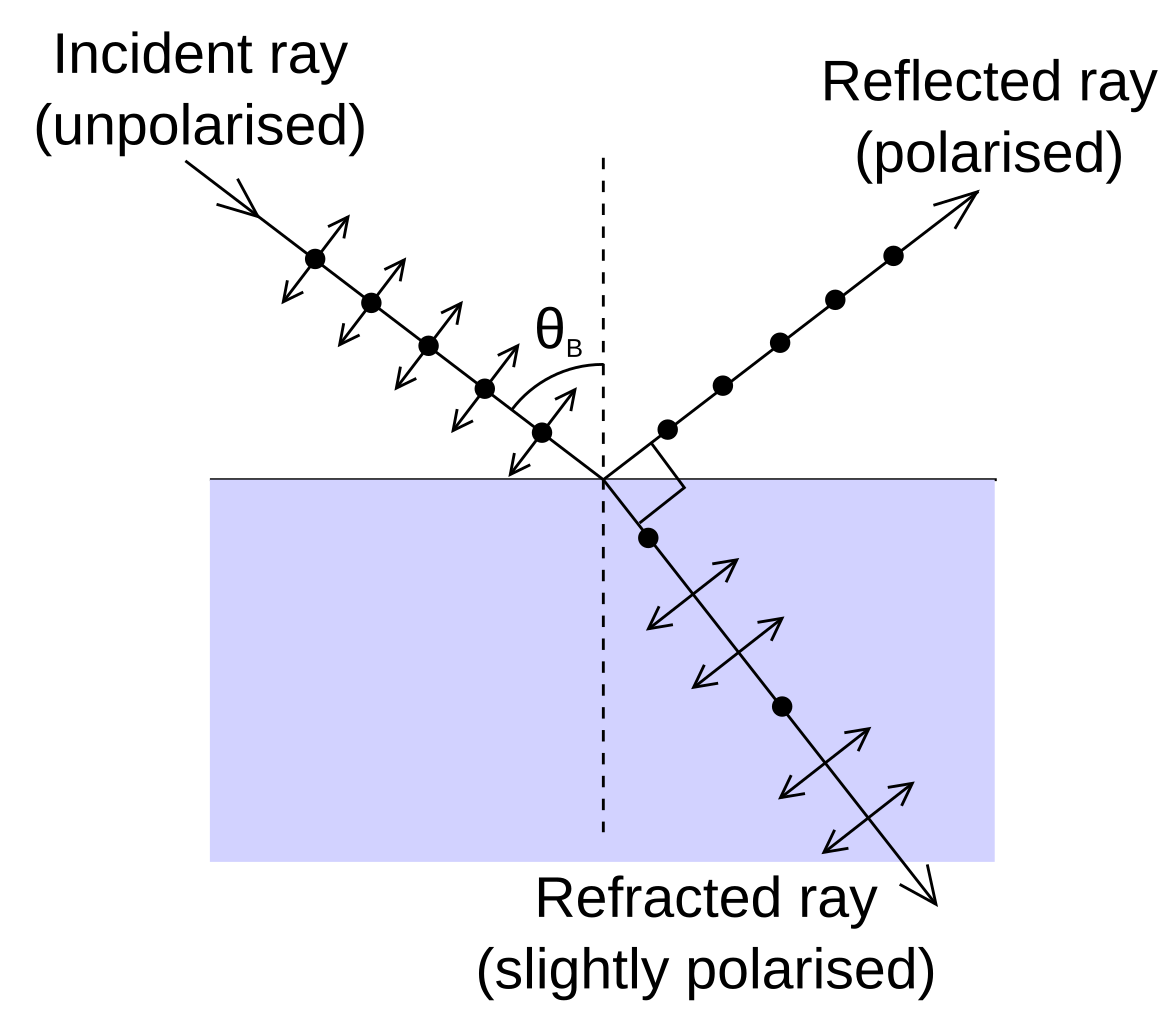
\includegraphics[width=0.25\textwidth]{slike/Brewsters-angle.svg.png}
    \caption{Brewster's angle }
    \label{fig:brewstr}
\end{figure}

\subsection{Linear polarization}
EM wave, shown on figure \ref{fig:linpol} is polarized linearly. 

\begin{figure}[h!]
    \centering
    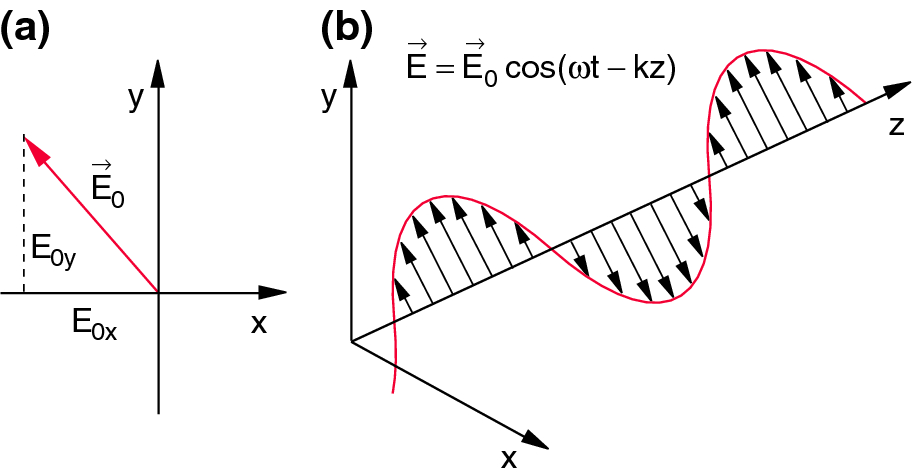
\includegraphics[width=0.5\textwidth]{slike/linpol.png}
    \caption{Linear polarization}
    \label{fig:linpol}
\end{figure}

Electric filed in $x,y$ directions can be described as:
\begin{align}
    E_x = E_{0x} cos(kz - \omega t)\\
    E_y = E_{0y} cos(kz - \omega t)
\end{align}
combined:
\begin{equation}
    E = (\vec{e}_x E_{0x} + \vec{e}_y E_{0y}) cos(kz - \omega t)
\end{equation}



\subsection{Circular polarization}
Circular polarization is shown on figure \ref{fig:cirpol}.
\begin{figure}[h!]
    \centering
    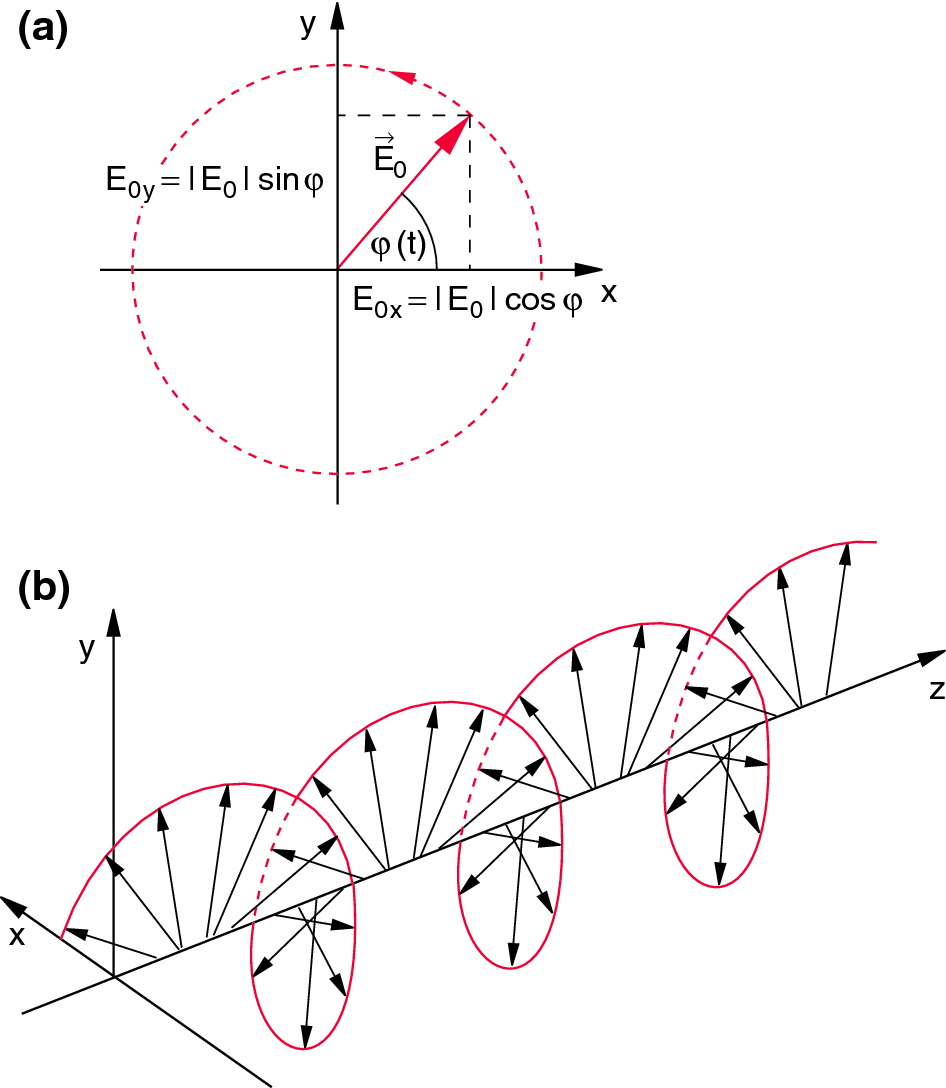
\includegraphics[width=0.35\textwidth]{slike/circpol.png}
    \caption{Circular polarization}
    \label{fig:cirpol}
\end{figure}

\begin{align}
    E_x = E_{0x} cos(kz - \omega t)\\
    E_y = E_{0y} cos(kz - \omega t + \frac{\pi}{2}) =  -E_{0y} cos(kz - \omega t)
\end{align}
combined (phase delay $\varphi = \frac{\pi}{2}$):
\begin{equation}
    \vec{E} = E_0 (\vec{e}_x cos(kz - \omega t) - \vec{e}_y sin(kz - \omega t))
\end{equation}

The delay $\varphi$, determines the way the light is polarized - clockwise or counterclockwise
polarization. 

When two EM-waves of different circular polarization are superimposed (interfere),
the result is linearly polarized light with the amplitude $2 E_0$.

\begin{align}
    \vec{E_1} = E_0 (\vec{e}_x cos(kz - \omega t) - \vec{e}_y sin(kz - \omega t))\\
    \vec{E_2} = E_0 (\vec{e}_x cos(kz - \omega t) + \vec{e}_y sin(kz - \omega t))\\
    \vec{E}_{res} = 2 E_0 \vec{e}_x cos(kz - \omega t)
\end{align}

In order to have circular polarization, $\varphi$ must be $0$\textdegree, $\pm 90$\textdegree, $180$\textdegree.

\subsection{Elliptical polarization}
When light polarization is \textbf{not} linear or circular, it is \textbf{elliptical}.
Such polarization is achieved when the phase difference of different waves is not $\varphi \ne 0, \pm \frac{1\pi}{2}
\pm \frac{2\pi}{2},\pm \frac{3\pi}{2}, \dots$. 

\subsection{Polarized and unpolarized light}
Any polarization can be seen as a superposition of two fundamental 
polarization types:
\begin{itemize}
    \item two orthogonal linear polarizations
    \item two counter-rotating circular polarizations
\end{itemize}

Unpolarized light contains waves polarized in different directions. Most light sources emit unpolarized light.

\textbf{Most lasers} emit \textbf{polarized} light due to their fundamental properties or design.
It is possible to rotate linear polarization, \textbf{without energy loss}, using a \textit{half-waveplate}. Converting circularly polarized light to linearly polarized light 
using a \textit{quarter-waveplate}.
\newpage
\chapter{Absorption and Emission}

\section{Absorption}
When a photon travels through matter - atoms - it can be absorbed, as shown on figure
\ref{fig:absorption1}.
\begin{figure}[h!]
    \centering
    \includegraphics[width=0.5\textwidth]{slike/absorption.pdf}
    \caption{Absorption of an electron}
    \label{fig:absorption1}
\end{figure}

There must be a \textbf{free orbital} with the right dipole moment that is energetically above the currently excited state and an 
exciting EM-wave with the correct energy (and $\lambda$).

\section{Emission}
Emission can be \textbf{spontaneous} or \textbf{stimulated}.




\subsection{Stimulated emission}
Stimulated emission, figure \ref{fig:stimem}, is same as time reversed absorption. There must be a free orbital with the correct dipole moment that is energetically
below the currently excited state and an exciting EM-wave with the correct energy (and $\lambda$).
Atom's orbital lifetime has no influence on wavelength of the emitted photon.

% \begin{itemize}
%     \item The charge distribution will first oscilate with the frequency of the incoming EM-wave
%     \item If the oscilatinating charge resembles a fitting orbital with a lower energy there is a chance that an electron will hop into this lower
%     energy orbital, it will emit a photon.
%     \item 
Emitted photon has the same: \begin{itemize}
        \item \textbf{wavelength } $\lambda$
        \item \textbf{frequency} $\nu$
        \item \textbf{polarization}
        \item \textbf{phase}
        \item \textbf{propagation direction}
    \end{itemize}
%\end{itemize}

Frequency of the emitted or absorbed EM-wave is proportional to the
energy difference between $\Delta E$ in the atomic levels according to equation \ref{eq:aeeq}.
\begin{equation}
    E_{photon} = \Delta E = E_2 - E_1 = h \cdot \nu
    \label{eq:aeeq}
\end{equation}
Where $h$ is the \textit{Planck constant}, which is equal to  $6.626 \times 10^{-34} \, \frac{J}{Hz}$ or $4.135 \times 10^{-15} \,\frac{eV}{Hz}$.


\subsection{Spontaneous emission}

Spontaneous emission, figure \ref{fig:spem}, is a process in which a quantum system - mulecule, atom, particle - 
transits from an excited state to a lower state.  When a photon is emitted douring spontaneous emisson, it has random \textbf{polarization}, \textbf{propagation direction} and \textbf{random phase}.
The range of emitted oscillations frequencies depends on the stability of atomic orbitals.
\begin{figure}[h!]
    \centering
    \begin{subfigure}{0.4\textwidth}
        \includegraphics[scale=1]{slike/spontem.pdf}
        \caption{Spontaneous emission}
        \label{fig:spem}
    \end{subfigure}
    \begin{subfigure}{0.4\textwidth}
        \includegraphics[scale=1]{slike/stimemm.pdf}
        \caption{Stimulated emission}
        \label{fig:stimem}
    \end{subfigure}
\end{figure}

There is always some spontaneous emission in a laser, it depends on the environment, laser ...


\subsection{Line broadening}

\textbf{Heisenberg's uncertainty} principle for energy and time is the law governing the relationship between orbital life times and frequencies, equation \ref{eq:heis}.
\begin{equation}
    \delta E \cdot \delta t = \frac{h}{4 \pi}
    \label{eq:heis}
\end{equation}

Where $h$ is the \textit{Planck constant}, $\delta t$ the lifetime of the excited state and $\delta E$ is the range of photon energies taht cen be emitted from an excited state.
Taking line broadening into account, the computation of photon energy $E_{photon}$ is now \ref{eq:ep2}.
Line broadening is represented by equation \ref{eq:dnu}.
\begin{equation}
    E_{photon} = \Delta E \pm \delta E = h (\nu \pm \delta \nu) \\
    \label{eq:ep2}
\end{equation}
\begin{equation}
    \delta \nu = \frac{1}{2 \pi \delta t}
    \label{eq:dnu}
\end{equation}

\newpage
\chapter{Lasering (and so on and so on)}

\section{Population and Rate equation}

\textbf{Population} means how many atoms of an atomic ensemble are in a certain \textbf{state}.
State refers to the energy level or orbital that electrons are in - such as ground state, $1^{st}$ orbital, $2^{nd}$ orbital, $\dots$

Number of atoms in a certain state can be described by the \textbf{rate equations}. Figure \ref{fig:rate} show the emission and absorption with the equations that 
are in the laser.

\begin{figure}[h!]
    \centering
    \includegraphics[width=0.95\textwidth]{slike/rate.pdf}
    \caption{Emission and absorption with equations}
    \label{fig:rate}
\end{figure}

Equation \ref{eq:rate_abs} calculates the state of population during \textbf{absorption}. Variable $q$ is equal to spectral photon energy density of input/incoming light. $N_i$ is
the population density of level $i$. Coefficients $A_{ij}$ and $B_{ij}$ are \textit{Einstein coefficients} for between levels.\\ \textit{Note:}$B_{ij} \;=\; B_{ji}$
\begin{equation}
    \frac{dN_1}{dt} = -N_1 q B_{12}
    \label{eq:rate_abs}
\end{equation}
Equation \ref{eq:rate_spem} shows the rate of \textbf{spontaneous emission}. It is \textit{not} dependent on $q$.

\begin{equation}
    \frac{dN_2}{dt} = -A_{21}N_2
    \label{eq:rate_spem}
\end{equation}
Equation \ref{eq:rate_stem} shows the rate of \textbf{stimulated emission}.
\begin{equation}
    \frac{dN_2}{dt} = -N_2 q B_{21}
    \label{eq:rate_stem}
\end{equation}

Relationship between $A_{21}$ and $B_{21}$ is $ \frac{A_{21}}{B_{21}} = \frac{8 \pi h \nu^3}{c^3} $.

Change of photon (population) density through propagation in $x$ direction through a
given population distribution $N_2$ and $N_1$  is called \textbf{Lambert-Beer law} - equation \ref{eq:lbl}.
\begin{eqnarray}
    q(x) = q_0 \cdot e^{\frac{B_{12} h \nu}{c}(N_2 -N_1)x}
    \label{eq:lbl}
\end{eqnarray}
In order to have light \textbf{amplification}, population $N_2$ must be bigger that $N_1$, this is called \textbf{inverse population}.

\section{Boltzmann distribution}
Figures \ref{fig:gdist} and \ref{fig:idist} show the ground (normal) and inverse population distribution.
\begin{figure}[h!]
    \centering
    \begin{subfigure}{0.4\textwidth}
        \includegraphics[scale=1]{slike/gdist.pdf}
        \caption{Equilibrium population}
        \label{fig:gdist}
    \end{subfigure}
    \begin{subfigure}{0.4\textwidth}
        \includegraphics[scale=1]{slike/idist.pdf}
        \caption{Inverse population}
        \label{fig:idist}
    \end{subfigure}
\end{figure}
 In $N_j - N_i < 0$, the population is in \textbf{thermodynamic equilibrium}, if $N_j - N_i > 0 $ in a laser
active medium we have \textbf{inverse population}.

Boltzmann distribution can be calculated as \ref{eq:boltz}.
\begin{equation}
    \frac{N_2}{N_1} = \frac{g_2}{g_1} exp(-\frac{E_2 - E_1}{kT})
    \label{eq:boltz}
\end{equation}
Where $E_i$ is the energy value of the state, $T$ is the absolute temperature,
$k$ is the \textit{Boltzmann constant},$k = 1.38 \times 10^{-23} \frac{J}{K} = 8.63 \times 10^{-5}\, \frac{eV}{K}$, and $g_i$ is the number of sublevels of state $i$.
For non-degenerate states $g_2 = g_1 = 1$.
In a two level system, inverse population is \textbf{not possible}:
\begin{gather}
    \frac{dN_1}{dt} = -N_1 q B_{12} + N_2 q B_{21} + A_{21} N_2 = q B_{12} (N_2 - N_1) + A_{21}N_2 \\
    \frac{dN_2}{dt} = +N_1 q B_{12} - N_2 q B_{21} - A_{21} N_2 = q B_{12} (N_2 - N_1) + A_{21}N_2 \\
    \frac{dN_2}{dt} = -\frac{dN_1}{dt}
\end{gather}
The fill up rate  is same as the depletion rate.
Inverse population is therefore \textbf{not possible}, there is no net optical gain.
To achieve inverse population, we need a higher level system.

\section{Three and four level systems}
Figure \ref{fig:3lvlsys} show the levels of a 3 level system and the transitions.

Transition $1$ shows the pumping of, transition $2$ is a radiationless transition, the $3$ transition is the laser transition.

Figure \ref{fig:4lvlsys} show a simplified 4 level system. Laser transition is between laser and depletion level, transition $3$. 

\begin{figure}[h!]
    \centering
    \begin{subfigure}{0.45\textwidth}
        \includegraphics[scale=0.75]{slike/3lvlsys.pdf}
        \caption{Three level system}
        \label{fig:3lvlsys}
    \end{subfigure}
    \begin{subfigure}{0.45\textwidth}
        \includegraphics[scale=0.75]{slike/4lvlsys.pdf}
        \caption{Four level system}
        \label{fig:4lvlsys}
    \end{subfigure}

\end{figure}

\section{Laser line broadening}

An ideal monochromatic wave has a \textbf{single } $\nu$ or $\lambda$ - spectral width is zero. 
In reality, every light source has a \textbf{spectral width greater than zero}.
Shape of the realistic spectrum is shown on figure \ref{fig:bls}. The shape is given by a density function.

\begin{figure}[h!]
    \centering
    \includegraphics[width=0.75\textwidth]{slike/lrb.pdf}
    \caption{Spectral line broadening}
    \label{fig:bls}
\end{figure}

Equation \ref{eq:linebroadening} show the relation between linewidth and frequency.
\begin{equation}
    \Delta \nu \approx \frac{c}{\lambda^2} \Delta \lambda
    \label{eq:linebroadening}
\end{equation}
Figure \ref{fig:lb} show line broadening effect in an energy(?) diagram.
\begin{figure}[h!]
    \centering
    \includegraphics[width=0.5\textwidth]{slike/linebroadening.pdf}
    \caption{Line broadening}
    \label{fig:lb}
\end{figure}

\subsection{Types of line-broadening}
Different line broadening mechanisms are shown on figure \ref{fig:chart_broad}.
\begin{figure}[h!]
    \centering
    \includegraphics[width=0.5\textwidth]{slike/chart_broadening.pdf}
    \caption{Chart of line broadening mechanisms}
    \label{fig:chart_broad}
\end{figure}

\subsubsection{Homogenous broadening}
\textbf{Lifetime broadening}\\
The \textbf{Heisenberg uncertainty principle}, $\delta E = \frac{h}{4 \pi \tau}$ relates the lifetime of a certain state $\tau$
with its energy. This broadening effect results in an unshifted Lorentzian profile.
Photon energy of a transition is $E_{photon} = E_2 - E_1 = h \cdot \nu$.
Lifetime broadening is calculated as \ref{eq:lftb}.
\begin{equation}
    \Delta \nu = \frac{1}{2 \pi} (\frac{1}{\tau_1} + \frac{1}{\tau_2})
    \label{eq:lftb}
\end{equation}
Factor $\frac{1}{2 \pi}$ depends on the shape of the curve or where it is measured.\\

% \subsubsection{Homogenous }
\textbf{Collision/pressure broadening}\\
Each particle collision can act as a trigger for a spontaneous decay, this happens to each particle regardless of its other
properties. Collision broadening is calculated as \ref{eq:cbrd}.
\begin{equation}
    \Delta \nu = \frac{f_{coll}}{\pi}
    \label{eq:cbrd}
\end{equation}

\textbf{Combined homogenous broadening} is $\Delta \nu_{hom} = \frac{1}{2}(\frac{1}{\tau_1} + \frac{1}{\tau_2} + 2 f_{coll})$.

\subsubsection{Inhomogenous broadening}
\textbf{Doppler broadening}\\
Doppler line broadening occurs due to the \textbf{Doppler shift} - $\Delta f_D$. The frequency changes according to equation \ref{eq:dopbr}.
\begin{equation}
    f_D = f_0 \pm (\frac{v}{c})\cdot f_0
    \label{eq:dopbr}
\end{equation}
Where $v$ is the speed of the observer, $c$ the speed of light and $f_0$ the original frequency.

\textbf{Combined inhomogenous broadening} is $\Delta \nu_{inh} = ?????$.
\newpage
\chapter{Interference}
We will consider plane wave in one dimension - figure \ref{fig:simplewave}.
Two (or more) such waves can have \textbf{constructive} or \textbf{destructive interference}.
Figure \ref{fig:posint} shows \textbf{constructive} interference, bot waves add, according to equation \ref{eq:posint}.
\begin{equation}
    A_{01} + A_{02}  = A_{01} \cdot sin(kx + \omega t) + A_{02} \cdot sin(kx + \omega t) = (A_{01}+ A_{02}) \cdot sin(kx + \omega t)
    \label{eq:posint}
\end{equation}
\begin{figure}[h!]
    \centering
    \includegraphics[width=0.75\textwidth]{slike/posint.pdf}
    \caption{Constructive interference}
    \label{fig:posint}
\end{figure}

\textbf{Destructive} interferance is shown on figure \ref{fig:negint}, equation is the same as \ref{eq:posint}, but due to the waves being in opposite phase
$(A_{01}+ A_{02})$ is equal to $(A_{01} - A_{02}) = 0$
\begin{figure}[h!]
    \centering
    \includegraphics[width=0.75\textwidth]{slike/negint.pdf}
    \caption{Destructive interference}
    \label{fig:negint}
\end{figure}

In both cases, waves have the same phase with different signs. When the phase shift is arbitrary,
interference still happens. 
Equation \ref{eq:interferance} is used to calculate the output.
\begin{equation}
    E(x,t) = \frac{E_0}{2} (e^{i(kx - \omega t + \varphi)} + e^{-i(kx - \omega t + \varphi)}) = E_0 \cdot cos(kx - \omega t + \varphi)
    \label{eq:interferance}
\end{equation}
Intensity is equal to $I(t) = E(t) + E(t)^*$. In case of two waves with equal frequency $E = E_1 + E_2$.
Total intensity if then \ref{eq:intI}.
\begin{equation}
    I = (E_1 + E_2) \cdot (E_1 + E_2)^* = I_1 + I_2 + 2 I_{12}\cdot cos(\varphi_2 - \varphi_1) = 2 A_1 A_2 \cdot cos(\varphi_2 - \varphi_1)
    \label{eq:intI}
\end{equation}
Resulting intensity depends only on phase relation between waves.  Figure \ref{fig:2Dint} show constructive and destructive interference between two 
wave sources.

\begin{figure}[h!]
    \centering
    \includegraphics[width=0.75\textwidth]{slike/2Dinterference.pdf}
    \caption{2D interference, source:wikipedia.com}
    \label{fig:2Dint}
\end{figure}

In order to get interference, waves must have the same \textbf{polarization}, otherwise interference will lead to a change in the state polarization.
Energy is \textbf{conserved} and redistributed between the minimum and maximum states, which are determined by the interferance.


\newpage
\chapter{Coherence}

To determine the interoperability - ability to interfere - of two EM-waves we compare them at
different \textbf{time} and \textbf{location}. Comparison is done using the \textit{correlation equation} - \ref{eq:correlation}.
\begin{equation}
    \int E_1(x,t) \cdot E_{2}^* (x',t+\tau) d\tau
    \label{eq:correlation}
\end{equation}

We will use some simplifications:
\begin{enumerate}
    \item Absorption works perfectly and is instantaneous
    \item Emitted EM-wave has the same direction, but a random phase
    \item EM-wave is infinite and has a random phase
    \item Wavelength $\lambda$ is not always the same - wavelength fluctuations
    \item Amplitude is not constant - power fluctuations 
\end{enumerate}
We can use the equation for a simplified wave $A(x,t) = A_0 cos(kx - \omega t + \varphi)$,
due to the simplifications 4. and 5., the $\omega t$ becomes the random component.
Connection between this and line-broadening/uncertainty means that the size of phase space in time and frequency
cannot be smaller than $\delta \nu \cdot \tau  \ge \frac{1}{4 \pi}$.
This phase space will not change unless it loses or gains energy.
Product $\delta \nu \cdot  \tau$ is also called \textbf{time-bandwidth product}.

Consequences of this are:
\begin{itemize}
    \item Transitions that are long-lived states provide better wavelength and intensity stability
    \item If $\delta \nu \cdot \tau >> \frac{1}{4\pi}$ wave will have \textbf{strong and random intensity fluctuations} $\rightarrow$ the wave will not interfere with itself
\end{itemize}
The ability of the wave to interfere is called \textbf{coherence}.
Coherence time is the duration during which all the emitted waves can interfere with each other, calculated by \ref{eq:tcoh}.
\begin{equation}
    \tau_{coh} = \frac{1}{\Delta \nu}
    \label{eq:tcoh}
\end{equation}
Where $\Delta \nu$ is measured at $FWHM$. \textbf{Coherence length} is a distance across two waves can interfere, calculated as \ref{eq:lcoh}.
\begin{equation}
    L_{coh} = c \cdot \tau_{coh}
    \label{eq:lcoh}
\end{equation}

Examples of coherence length for different light sources are show in table \ref{tab:clen}.
\begin{table}[h!]
    \centering
    \begin{tabular}{|c|c|c|}
        \hline
        Light source & Wavelength $\lambda$ & Coherence length $L_{coh}$ \\
        \hline
        HeNe single mode & 633 nm & 100 m \\
        \hline
        Argon ion & 488/515 nm & 20 mm \\
        \hline
        GaAIAs, Single mode& 670-905 nm & 3 m\\
        \hline
        Sodium lamp & 2 lines @ 589 nm & 0.6mm \\
        \hline  
        Sunlight & 500 nm & 1 $\mu m$ \\
        \hline     
    \end{tabular}
    \caption{Coherence length}
    \label{tab:clen}
\end{table}

\section{Beam Parameter Product}
Beam parameter product  or BPP is defined as a product of \textbf{beam radius} at waist and \textbf{beam divergence}.

In equation $A(r,t) = A_0 cos(kr - \omega t + \varphi)$ - (\ref{eq:wave}), we have the factors $k,r$. We wish to find a connection between them.
The factors $k$ and $r$ are connected via:
\begin{itemize}
    \item Position-momentum uncertainty: $\Delta x \Delta p_x \ge \frac{h}{4 \pi}$
    \item Fourier transition: space $\leftrightarrow$ spatial frequency (wave vector $k$)
\end{itemize}

Beam parameter product is : $\delta k \cdot \delta r \ge \, const$

Beam parameter product and time-bandwidth product are a consequence of same fundamental laws, meaning that BPP cannot be smaller
than a certain value, which means that light cannot be focused below a certain focal spot size.

%maybe add a picture?


\newpage
\chapter{Resonator}
Lasering principle in a resonator with laser active medium which achieves population inversion:
\begin{enumerate}
    \item Spontaneous emission $\rightarrow$ incoherent, unpolarized light with random direction, phae, polarization. Wavelength is given by the lifetime of excited state
    \item Spontaneous emission will cause stimulated emission (amplified spontaneous emission ASE)
    \item ASE-light still has the same properties - unpolarized and incoherent 
\end{enumerate}
To get a better coherence, a \textit{feedback} mechanism is required - we use a \textbf{resonator}.
Mirrors feed back spontaneous emission and ASE to the laser medium and select a certain propagation direction.
Show on figure \ref{fig:res1}. We assume that the inverse population is kept by continuous laser pumping. Light reflected from the mirrors causes stimulated emission. Light with direction unsuported by mirrors leaves the resonator,
stimulated emission amplifies the \textit{allowed} directions over several cycles. 

\begin{figure}[h!]
    \centering
    \includegraphics[width=0.5\textwidth]{slike/res1.pdf}
    \caption{Simple resonator}
    \label{fig:res1}
\end{figure}

\textbf{Laser resonator}:
\begin{itemize}
    \item Intensity of light propagating in supported direction by resonator mirrors increases very fast 
    \item Propagation direction inside the laser resonator is fixed
    \item Incidence angles are fixed
    \item \textbf{Polarization with the smallest losses and largest gain wins}
    \item Time bandwidth product drops to its minimal possible value
\end{itemize}

\section{Spectral properties}
In a resonator only a standing waves with integer number $q$ of half-wavelength are possible.
Number $q$ depends on length of a resonator $L$ and $lambda$ - equation \ref{eq:res1}.
\begin{equation}
    L = q \cdot \frac{\lambda}{2}
    \label{eq:res1}
\end{equation}
Frequency separation between modes is calculated by the equation \ref{eq:res2}.
\begin{equation}
    \Delta \nu = \frac{c}{2 n L}
    \label{eq:res2}
\end{equation}
Where $n$ is the average index of refraction in a resonator. 
Figure \ref{fig:resmodes} show longitudinal modes in a resonator.
\begin{figure}[h!]
    \centering
    \includegraphics[width=0.5\textwidth]{slike/modes.pdf}
    \caption{Modes in a resonator}
    \label{fig:resmodes}
\end{figure}
Frequency separation is shown on figure \ref{fig:freqsep}.
\begin{figure}[h!]
    \centering
    \includegraphics[width=0.5\textwidth]{slike/deltalambda.pdf}
    \caption{$\Delta \lambda$ and $\Delta \nu$ }
    \label{fig:freqsep}
\end{figure}

\section{Time-bandwidth product of a laser resonator}

We know that in resonator, only certain frequency are allowed and that real resonators have losses, due to imperfections
in the mirrors. In the ideal case, we can get the time-bandwidth product from the frequency bandwidth from the extents (razsežnosti), which are given by the time duration of the photons ($\tau$)?????

%what are extents??

\section{Losses}
Figure \ref{fig:schres} show a simplified resonator. 
\begin{figure}
    \centering
    \includegraphics[width=0.5\textwidth]{slike/resonator_losses.pdf}
    \caption{Lossy resonator}
    \label{fig:schres}
\end{figure}
We calculate \textit{one round trip} losses with equation \ref{eq:losses}. Constants and variables are shown in table \ref{tab:losses}.
\begin{equation}
    R_1 R_2 e^{2 \alpha_m L_m} = e^{-2 \alpha_m L_m + ln(R_1 R-2)} = e^{2 \alpha_r L_R}
    \label{eq:losses}
\end{equation}

\begin{table}[h!]
    \centering
    \begin{tabular}{|l|p{2in}|}
        \hline
        $R$ & Mirror reflectivity \\
        $\alpha_m$ & Losses in gain medium \\
        $L_m$ & Gain medium length\\
        $L_R$  & Resonator length \\
        \hline
    \end{tabular}
    \caption{Constants}
    \label{tab:losses}
\end{table} 
For a free space resonator $\alpha_m L_m << 1$, $R_1 R_2 e^{2 \alpha_m L_m} \approx R_1 R_2 \cdot 1 =  e^{2 \alpha_r L_R}$, from which  we get 
$\alpha_r = -\frac{ln(R_1 R_2)}{2 L_R}$.
Time dependant energy loss in a resonator can be expressed as $E(t) = E_0 \cdot e^{\alpha_r c t}$. Distance $x$ is a $x_P = x \tau = \frac{1}{\alpha_r}$ is the characteristic propagation length.
Time $\tau$ is a lifetime unit of a photon in the resonator, calculated as $\tau_P = \frac{1}{\alpha_r \cdot c}$.

Resonator line width is $\delta \nu = \frac{1}{2 \pi \tau_P}$

\section{Resonator with laser active medium}
Laser emits radiation in a comb of discrete frequencies, for a majority of applications, lasers can be 
treated as monochromatic radiation sources. Exceptions are interferometric applications, such as holographic systems or ultrafast lasers.
Figure \ref{fig:lamr} show the possible frequencies in a laser resonator with laser active medium.

\begin{figure}[h!]
    \centering
    \includegraphics[width=0.3\textwidth]{slike/activemediumresonator.pdf}
    \caption{Laser output spectrum}
    \label{fig:lamr}
\end{figure}

Laser oscillations can only be build-up for modes satisfying gain $G > 1$ for the condition \ref{eq:Gainresonator}.
\begin{equation}
    G = R_1 R_2 e^{2(g(\nu) - \alpha) L_m} \ge 1
    \label{eq:Gainresonator}
\end{equation}
Where $g(\nu)$ is a gain coefficient, which is a function of frequency $\nu$.
Gain factor is show in figure \ref{fig:gainfunc}.
\begin{figure}[h!]
    \centering
    \includegraphics[width=0.4\textwidth]{slike/gainfunc.pdf}
    \caption{Gain function}
    \label{fig:gainfunc}
\end{figure}

\section{Stability of resonators}
Resonator can be:
\begin{table}[h!]
    \begin{tabular}{l p{5in}}
        stable & light does not leave resonator after infinite number of reflections\\
        unstable & light leaves resonator after a certain number of reflections
    \end{tabular}
\end{table}

Figure \ref{fig:resstab} shows stable and unstable resonator.
\begin{figure}[h!]
    \centering
    \includegraphics[width=0.5\textwidth]{slike/typres.pdf}
    \caption{Stable and unstable resonator}
    \label{fig:resstab}
\end{figure}

Stable resonator will have a shorter bandwidth. Resonator is described by parameters shown in table \ref{tab:resparms}. Shown on figure 
\ref{fig:resstab}.
\begin{table}[h!]
    \centering
    \begin{tabular}{|l| p{2in}|}
        \hline
        L & mirror separation \\
        $r_i$ & mirror radius of curvature\\
        $d_{s1}$ & mirror diameter \\
        \hline
    \end{tabular}
    \caption{Resonator parameters}
    \label{tab:resparms}
\end{table}

\subsection{Resonator Configuration}
Resonator configurations, shown on figure \ref{fig:resconf}, influence resonator stablility.
\begin{figure}[h!]
    \centering
    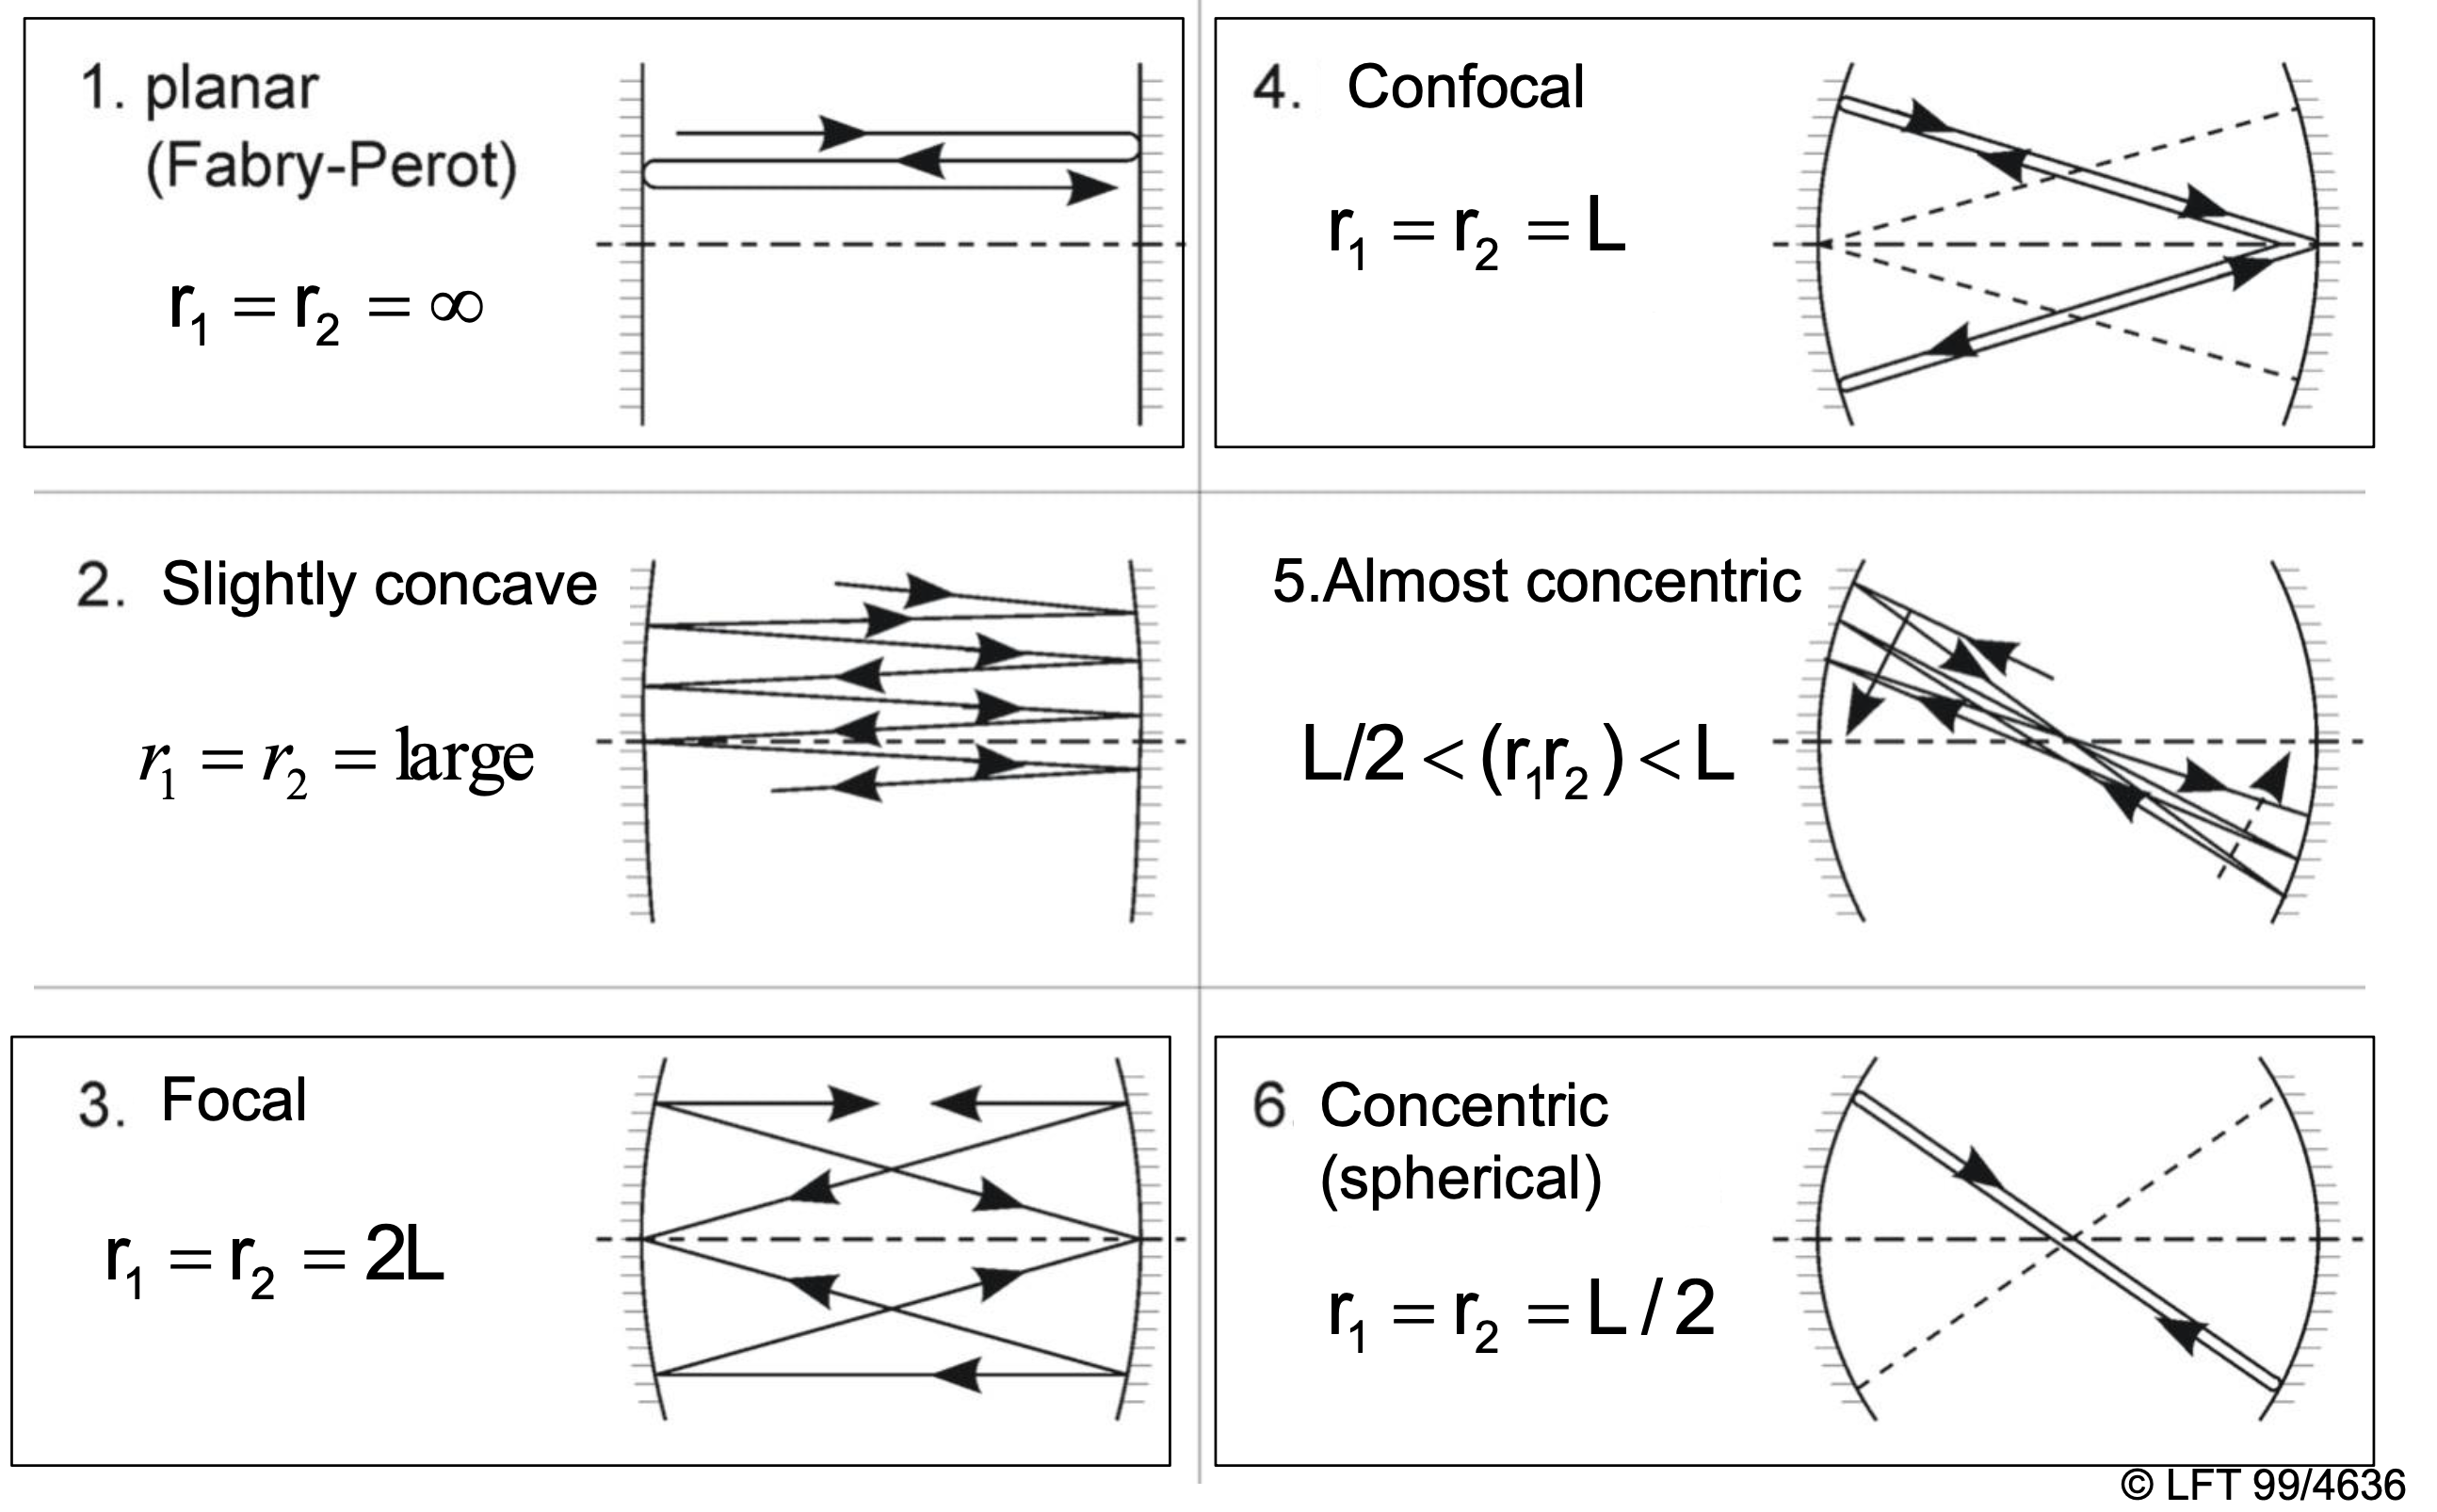
\includegraphics[width=0.75\textwidth]{slike/res_configs.png}
    \caption{Resonator configuration. \textit{Source: lecture notes} }
    \label{fig:resconf}
\end{figure}
To describe the resonator, we can use the \textit{general (ABCD matrix)} or a \textit{simplified approach (g-parameters)}.
General approach is necessary for free space beam propagation, compared to g-parameters, it is more computaionaly expensive.
Simplified approach can only be used for two mirror resonators.

\subsubsection{Generalized approach}
Generalized approach - ABDC matrix formalism or raytracing is an approach that we use on more complex resonators - more than \textit{two mirrors}.

Mirrors can be described as lenses, simply by switching to a suitable coordinate system. To describe an optical beam or ray at any position,
we can use its position $x$ and its angle to optical axis $\alpha$. State of beam is therefore given by a vector $\begin{pmatrix}
    x\\ \alpha \end{pmatrix}$.



Beam propagation through mirror/lens consists of three steps:
\begin{table}[h!]
    \centering
    \begin{tabular}{|p{2in}|p{2in}|p{2in}|}
       \hline
        Propagation through \textit{air} \newline(parameter: distance) &
         Propagation through \textit{mirror/lens}\newline (parameter: focal length) & 
         Propagation through \textit{air}\newline (parameter: distance)\\
        \hline
    \end{tabular}
\end{table}
Effects of lens or mirror on a beam are shown of figure \ref{fig:eff}.
\begin{figure}[h!]
    \centering
    \includegraphics[width=0.9\textwidth]{slike/lenseff2.pdf}
    \caption{Effect of  lens/mirror}
    \label{fig:eff}
\end{figure}
Beam angle changes depending on focal length $f$, on position $x$ at which the beam arrives at the lens and the angle that a beam has
in front of the lens $\alpha_{in}$.
For center ray - blue line on figure \ref{fig:eff} - the beam leaves the lens at the same position, $x_{in} = x_{out}$, but the beam angle $\alpha$ changes.
Change of $\alpha$ depends on:
\begin{itemize}
    \item focal length $f$
    \item on position $x$ at which the beam arrives at the lens
    \item on the initial $\alpha_{in}$ in front of the lens 
\end{itemize}
Exiting angle $\alpha_{out}$ is calculated by the equation \ref{eq:aout}.
\begin{equation}
    \alpha_{out} = -\frac{x_{in}}{f} + \alpha_{in}
    \label{eq:aout}  
\end{equation}
Position of exiting beam changes according to the input angle $\alpha_{in}$ and propagation distance $L$, equation \ref{eq:xout}.
\begin{equation}
    x_{out} = x_{in} + L \cdot \alpha_{in}
    \label{eq:xout}
\end{equation} 

To simplify the notation, we can use matrices.
Beam propagation \textbf{through air}, can be written as shown in equation \ref{eq:mair}.
\begin{equation}
    \begin{pmatrix}
        x_{out} \\ \alpha_{out}
    \end{pmatrix} = \begin{pmatrix}
        x_{in} + L \alpha_{in} \\ \alpha_{in}
    \end{pmatrix} = \begin{pmatrix}
        1 & L \\ 0 & 1
    \end{pmatrix} \begin{pmatrix}
        x_{in} \\ \alpha_{in}
    \end{pmatrix}
    \label{eq:mair}
\end{equation}
Propagation \textbf{through mirror/lens}, can be wirtten as equation \ref{eq:mlens}.
\begin{equation}
    \begin{pmatrix}
        x_{out} \\ \alpha_{out}
    \end{pmatrix} =     \begin{pmatrix}
        x_{in} \\ -\frac{x_{in}}{f} \alpha_{in}
    \end{pmatrix}  = \begin{pmatrix}
        1 & 0 \\ -f^{-1} & 0
    \end{pmatrix} \begin{pmatrix}
        x_{in} \\ \alpha_{in}
    \end{pmatrix}
    \label{eq:mlens}
\end{equation}
Where $f_{mirror}$ is equal to $\frac{R_{mirror}}{2}$.


\textbf{ABCD formalism}

In equations \ref{eq:mair} and \ref{eq:mlens} we have defined two matrices. A matrix for free space propagation and a matrix for 
lens/mirror. 
Free space propagation matrix, shown in \ref{eq:fspm} and a matrix for lens/mirror propagation, shown in \ref{eq:mlpm}.
\begin{equation}
    P(L) =\begin{pmatrix}
        1 & L \\ 0 & 1
    \end{pmatrix}
    \label{eq:fspm}
\end{equation}

\begin{equation}
    M(f) = \begin{pmatrix}
        1 & 0 \\ -\frac{1}{f} & 0
    \end{pmatrix}
\label{eq:mlpm}
\end{equation}

Each path can be described as a multiplication of matrices, in the reverse order of light propagation, as shown in figure \ref{fig:abcdl}.
\begin{figure}[h!]
    \centering
    \includegraphics[width=0.7\textwidth]{slike/ABCD_lens.pdf}
    \caption{Propagation description by matrix multiplication}
    \label{fig:abcdl}
\end{figure}

Propagation inside the resonator can be simplified further - path is always the same, so we can introduce a new matrix $R$,
which is equal to the path of the light, for example for a resonator mirror-air-mirror-air, path  can be written as $R = P \cdot M_2 \cdot P \cdot M_1$.
For each cycle the light makes, we multiply the matrix $R$ by its self - equation \ref{eq:path}.
\begin{equation}
    \begin{pmatrix}
        x_{out} \\ \alpha_{out}
    \end{pmatrix} = R^n \cdot \begin{pmatrix}
        x_{in} \\ \alpha_{in}
    \end{pmatrix} = \prod_{1}^{n} R \cdot \begin{pmatrix}
        x_{in} \\ \alpha_{in}
    \end{pmatrix}
    \label{eq:path}
\end{equation}
\textit{Note: in $R^n$ is not exponent, but the amount of multiplications!}\\

For true resonator stability $n$ should be able to go to infinity without increasing the output postion or output angle.
Stability for a single cycle is calculated by the equation \ref{eq:ssc}.
\begin{equation}
    \vec{b}_{out} = R \cdot \vec{b}_{in} = \lambda \cdot  \vec{b}_{in}
    \label{eq:ssc}
\end{equation}
Beam parameter $b$ is the eingenvector of matrix $R$, $\lambda$ is the eigenvalue of matrix $R$,$0 \le \lambda \le 1$.
We can also state: $R \cdot \vec{b} = \lambda \cdot \vec{b}$.

To find the eigenvalues of in problems such as $R \cdot \vec{b} = \lambda \cdot \vec{b}$, we can find both eigen values $\lambda_{\pm}$ by solving the equation \ref{eq:eigval}.
\begin{equation}
    \lambda_{\pm} = \frac{A + D}{2} \pm \sqrt{(\frac{A+D}{2})^2 - det(R)}
    \label{eq:eigval}
\end{equation}
Where $R = \begin{pmatrix}
    A & B \\ C&D
\end{pmatrix}$. In case the resonator only consist of two mirrors, we derive the simpified approach.

\subsubsection{Simplified approach}
In case of resonator with only two mirrors, we can calculate the stability by equation \ref{eq:sr1}.
\begin{equation}
    0 \le g_1 g_2 \le 1
    \label{eq:sr1}
\end{equation}
Where $g_1 = 1 - \frac{1}{R_1}$ and $g_2 = 1 - \frac{1}{R_2}$, $R_i$ is the mirror curvature.
\newpage
Stability of a simplified resonator is shown in figure \ref{fig:slr}.
\begin{figure}[h!]
    \centering
    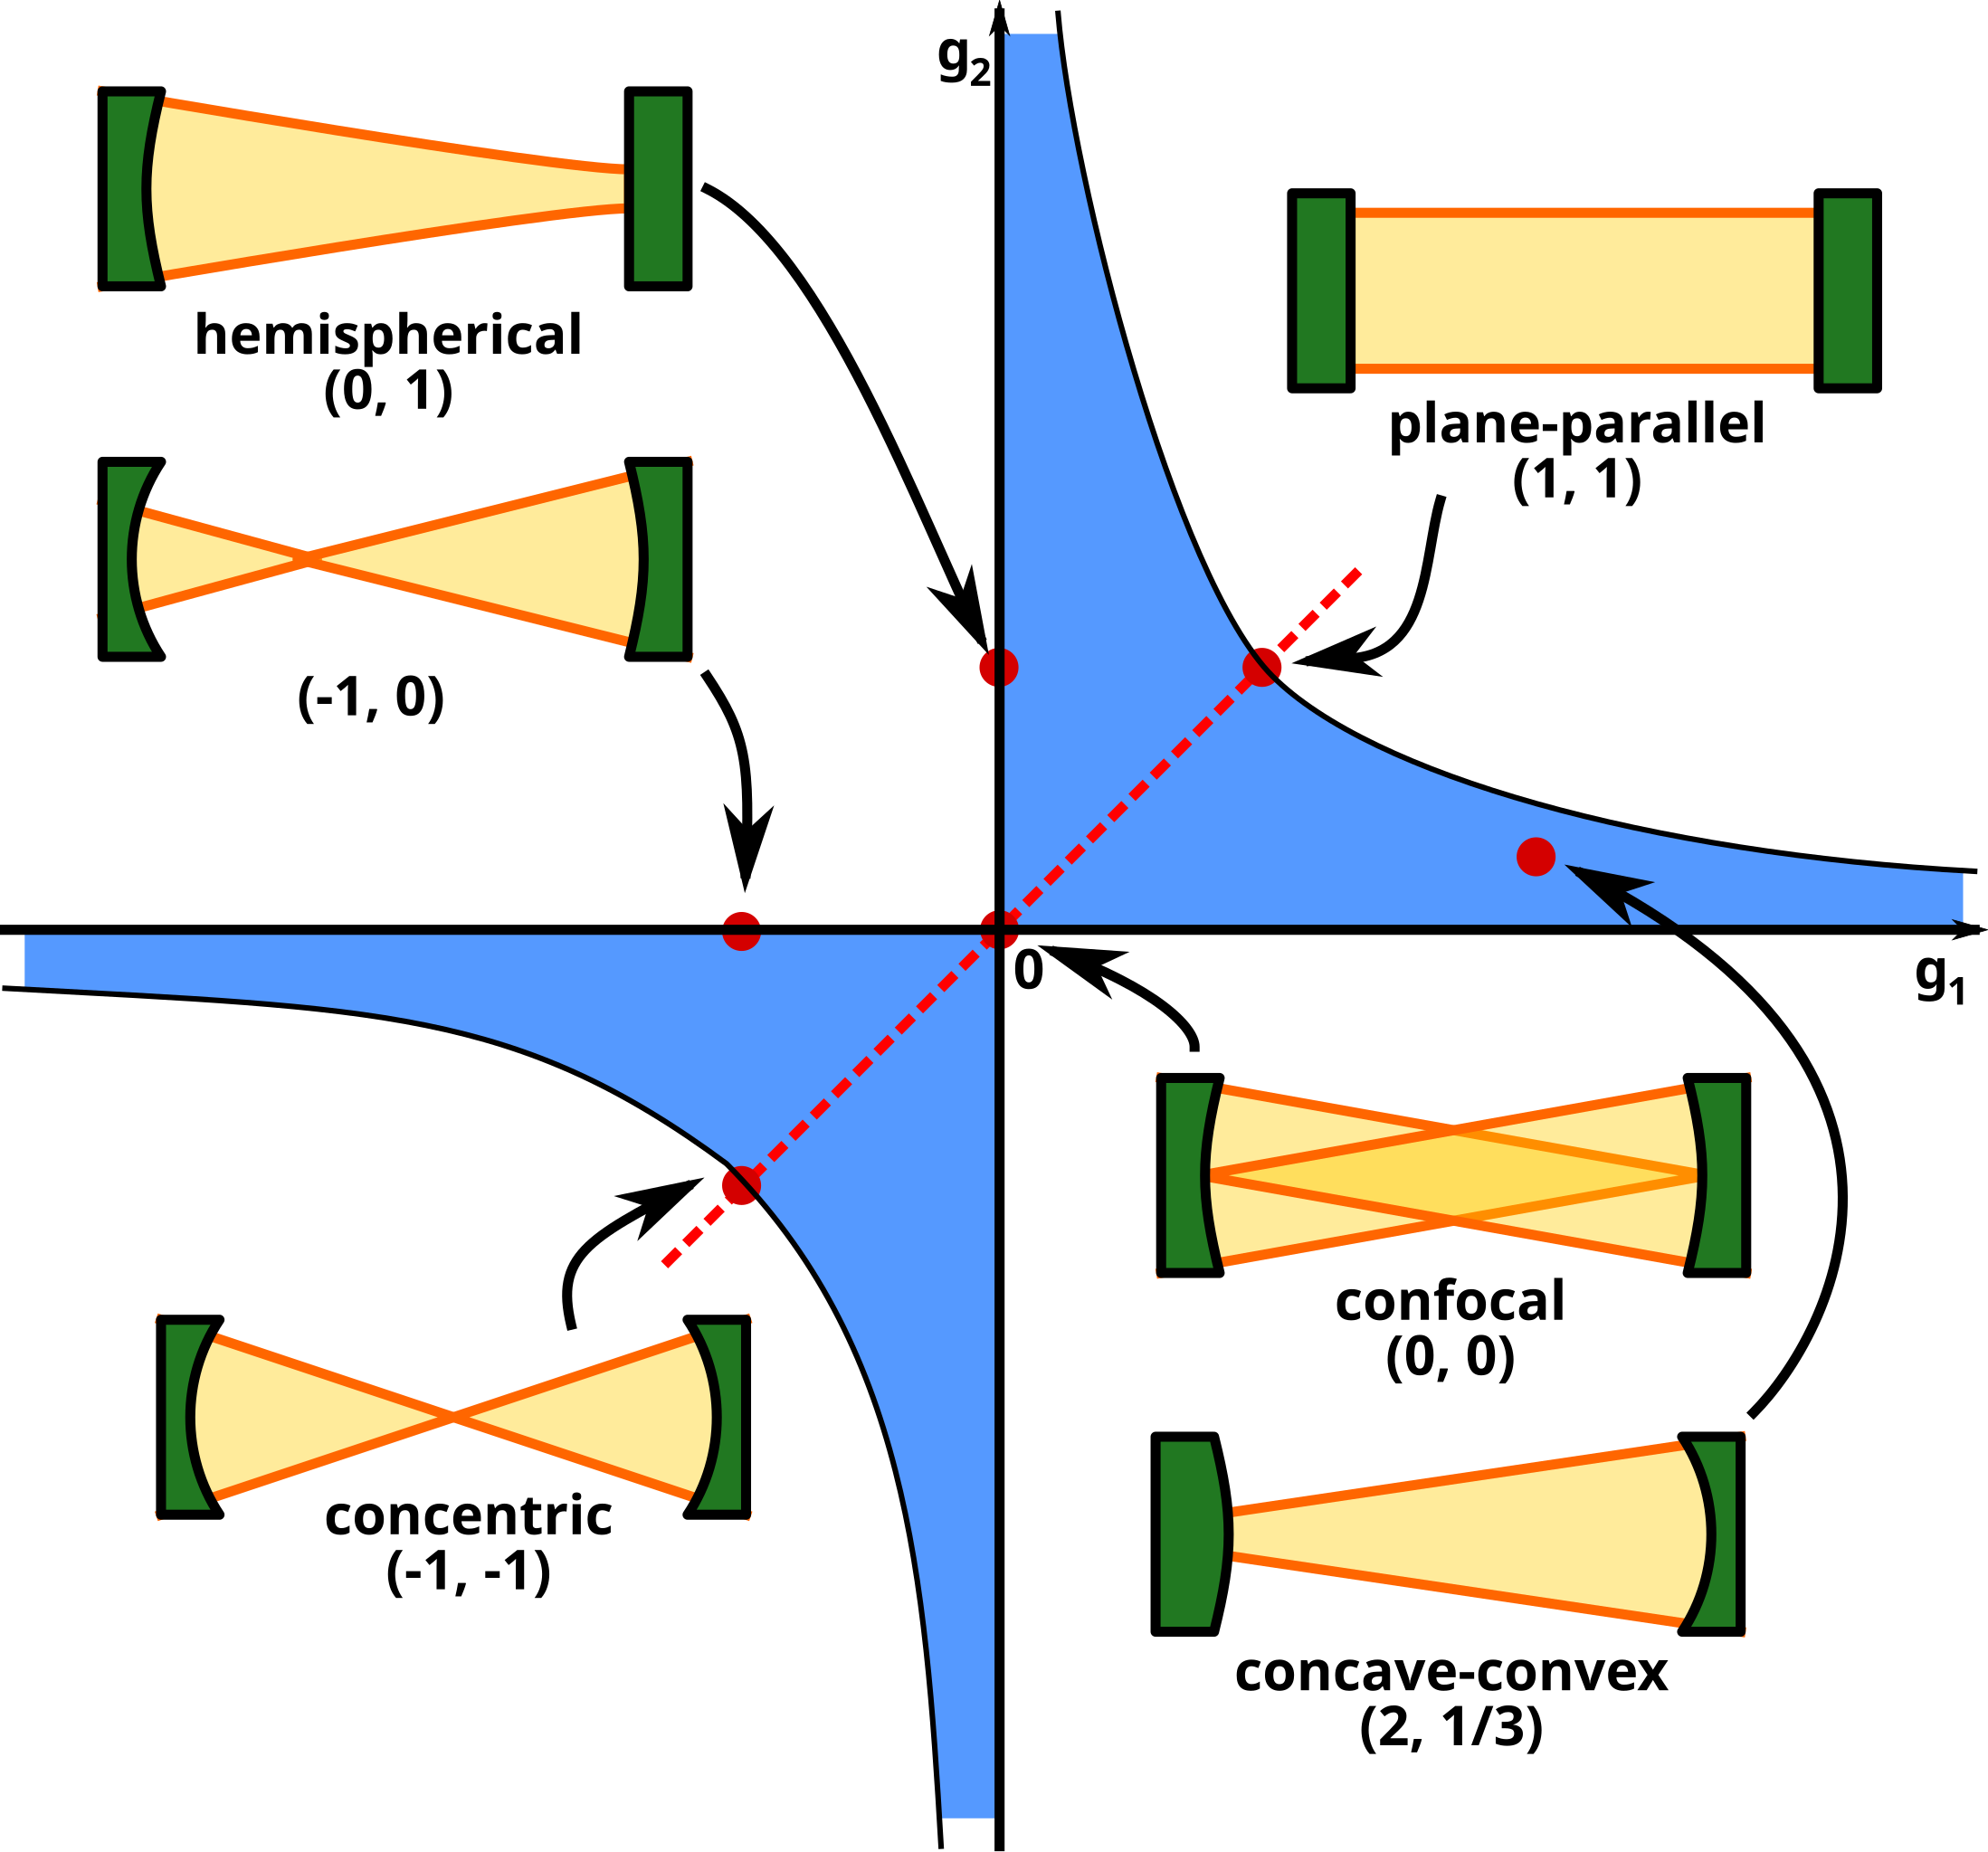
\includegraphics[width=0.5\textwidth]{slike/Laser_resonator_stability.png}
    \caption{Resonator stability}
    \label{fig:slr}
\end{figure}

We can use both \textbf{stable} and \textbf{unstable} resonators, stable resonator provide small beam parameter product and good beam quality.
Unstable resonators provide large beam parameter product, their advantage is, that they do not require a transmissive element.
\newpage
\chapter{Beam profile}

\section{Slit experiment}
Figure \ref{fig:slit_photon} shows a photon, with two dimensions.
\begin{figure}[h!]
    \centering
    \includegraphics[width=0.35\textwidth]{slike/slit_photon.pdf}
    \caption{Photon}
    \label{fig:slit_photon}
\end{figure}
Heisenberg's uncertainty principle, equation \ref{eq:slt_hup}, shows that as the spatial distribution of EM waves
becomes more and more constrained the BPP must increase to preserve the minimum product.
\begin{equation}
    \Delta x \Delta p \ge \frac{h}{4 \pi}
    \label{eq:slt_hup}
\end{equation}

\section{Diffraction at a slit}
Diffraction of a monochromatic plane beam at a slit is shown in figure \ref{fig:slit1}.
\begin{figure}[h!]
    \centering
    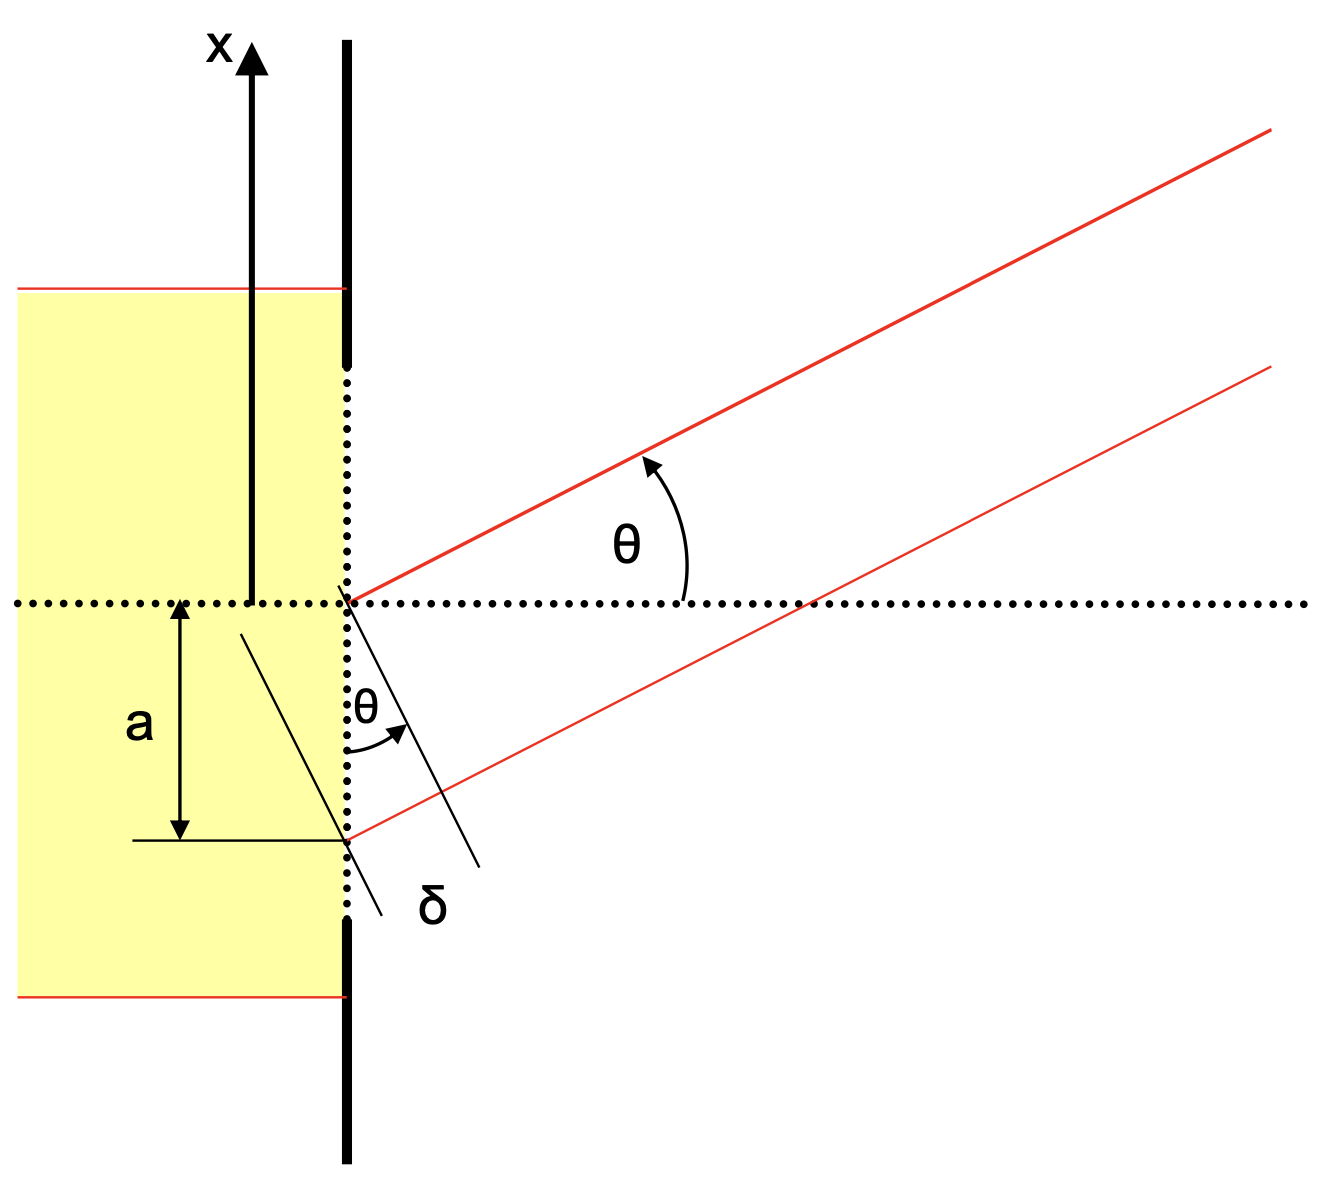
\includegraphics[width=0.35\textwidth]{slike/slit1.png}
    \caption{Diffraction at a slit}
    \label{fig:slit1}
\end{figure}
Another beam will have a path length difference of $\delta$, where $\delta = a \cdot sin(\theta)$, and a phase difference
of $\varphi = 2 \pi \frac{\delta}{\lambda} = \frac{2 \pi}{\lambda} \cdot a \cdot sin(\theta)$.
Sum of electric fields \ref{eq:sef}.
\begin{equation}
    \begin{aligned}
    E_{\sum} = E e^{i(k_z \cdot z + k_x \cdot x - \omega t)} + E e^{i(k_z \cdot z + k_x \cdot x - \omega t + \varphi)} =
    E e^{i(k_z \cdot z + k_x \cdot x - \omega t)} + E e^{i(k_z \cdot z + k_x \cdot x - \omega t + 2\pi \frac{\delta}{\lambda})} = \\
    E e^{i(k_z \cdot z + k_x \cdot x - \omega t)} + E e^{i(k_z \cdot z + k_x \cdot x - \omega t + \frac{2 \pi}{\lambda} \cdot a \cdot sin(\theta))} =  E_0(\vec{r},t) (1 + e^{i \frac{2\pi}{\lambda}a sin(\theta)}) 
    \end{aligned}
    \label{eq:sef}
\end{equation}

Interference for many beams, can be written as \ref{eq:imbd}.
\begin{equation}
    E_{\sum} = E_0(\vec{r},t) + \sum_{k=1,2,3...} E_0(\vec{r},t) e^{i\frac{2\pi}{\lambda}a_k sin(\theta)} =\sum_{k} E_0(\vec{r},t) e^{i\frac{2\pi}{\lambda}a_k sin(\theta)}
    \label{eq:imbd}
\end{equation}

For infinitely many beams the sum transitions to integration, as show in in equation \ref{eq:imb}.
\begin{equation}
    E_{\sum}(\vec{r},t) = \int_{-a_{max}}^{+a_{max}} E_0(\vec{r},t) e^{i\frac{2\pi}{\lambda} x sin(\theta)} dx
    \label{eq:imb}
\end{equation}
where $k_x(\theta) = \frac{2\pi}{\lambda} sin(\theta) = k_0 sin(\theta)$ and $E_0(\vec{r},t) = E e^{i(k_0 \cdot cos(\theta) \cdot z + k_0 \cdot sin(\theta) - \omega t)}$,
we can rewrite $E e^{i(k_0 \cdot cos(\theta) \cdot z + k_0 \cdot sin(\theta) - \omega t)} = E(\vec{r},t) e^{i(\frac{2\pi}{\lambda}x sin(\theta))}$ which is equal to
$E e^{i(k_0 \cdot cos(\theta) \cdot z - \omega \cdot t)} e^{i \cdot k_x(\theta) \cdot x}$. Combined we get the equation \ref{eq:fts}.
\begin{equation}
    E_{\sum} (\vec{r},t, \theta) = \int_{-a_{max}}^{+a_{max}} E_0(\vec{r},t) e^{i\cdot k_x(\theta) \cdot x} dx
    \label{eq:fts}
\end{equation}
We get symmetric \textbf{Fourier transform}. Table \ref{tab:ftp} shows the properties of the Fourier and inverse 
Fourier transform.
\begin{table}[h!]
    \begin{tabular}{|l|l|}
        \hline
        Forward transformation & Inverse transformation \\
        \hline
        time domain $\rightarrow$ frequency domain & time domain $\leftarrow$ frequency domain\\
        spatial domain $\rightarrow$ spatial frequency (angles) &spatial domain $\leftarrow$ spatial frequency\\
        $\hat{x}(\omega) = \mathcal{F}(x(t)) = \frac{1}{\sqrt{2\pi}} \int_{-\inf}^{\inf}x(t)e^{-i\omega t}dt$& $x(t) = \mathcal{F}^{-1}(\hat{x}(\omega))
        = \frac{1}{\sqrt{2\pi}} \int_{-\inf}^{\inf} \hat{x}(\omega)e^{i\omega t} d\omega$\\
        \hline
    \end{tabular}
    \caption{Properties of FT transform}
    \label{tab:ftp}
\end{table}

\subsection{Diffraction at rectangular aperture}
Intensity along $x$ axis is $I(\theta) = I_0 (sinc(\frac{A}{2} k sin(\theta)))^2$, with $sinc(x) = \frac{sin(x)}{x}$ 
and $k = \frac{2\pi}{\lambda}$($\pi$ phase shift), and $A$ the size of aperture.
Result of diffraction at a square aperture is shown on figure \ref{fig:squareaprture}.
\begin{figure}[h!]
    \centering
    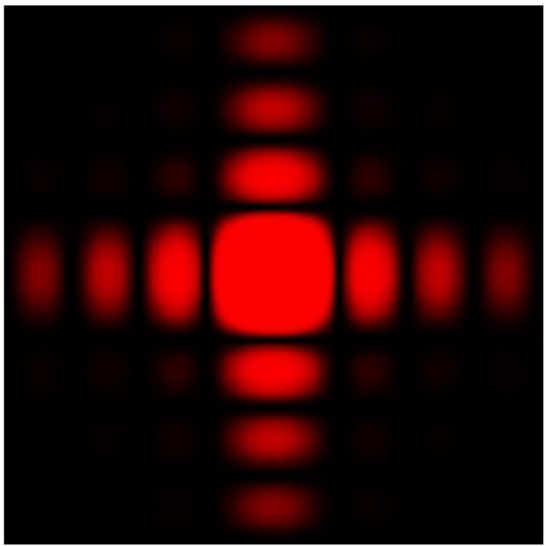
\includegraphics[width=0.15\textwidth]{slike/squareAdiff.png}
    \caption{Diffraction on square aperture. \sln}
    \label{fig:squareaprture}
\end{figure}

\subsection{Diffraction at round aperture}
Intensity along $x$ axis is given by \textit{Bessel J function} of the first kind $J_1(r)$. Equation \ref{eq:ira}
\begin{equation}
    I(\theta) = I_0 \left[\frac{2 J_1(\frac{A}{2} k sin(\theta))}{\frac{A}{2} k sin(\theta)}\right]^2
    \label{eq:ira}
\end{equation}
The lens allows us to observe at close distance, what we could see at the infinity. Figure \ref{fig:radf}.
\begin{figure}[h!]
    \centering
    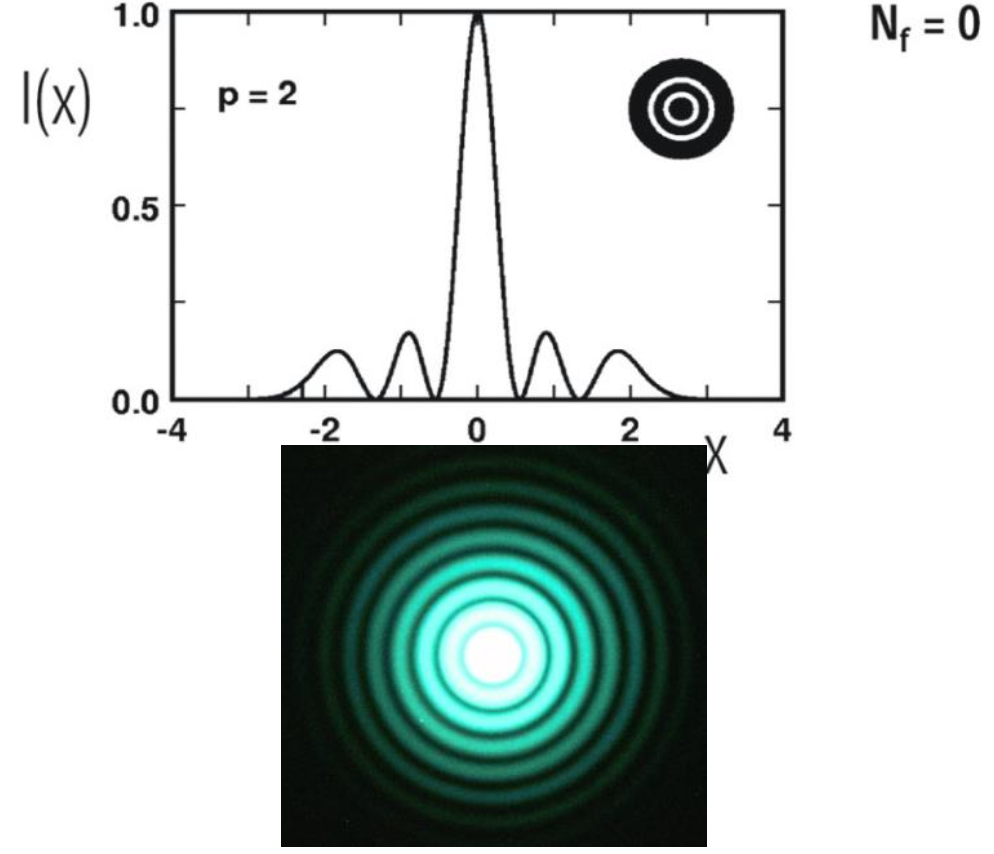
\includegraphics[width=0.25\textwidth]{slike/difSslt.png}
    \caption{Diffraction at round slit}
    \label{fig:radf}
\end{figure}

\subsection{Diffraction at resonator mirrors}
Diffraction on a mirror depends on mirror shape:
\begin{itemize}
    \item Plane mirrors - beam diffracts in the far field
    \item Concave mirrors - beam diffracts near the focal spot
\end{itemize}
In both cases, diffraction is given by the Fourier transform of mirror's aperture.
If beam intensity is homogeneous we have $sinc$ or $Bessel $ like diffraction patterns.

%333pp
\section{Fresnel number}
Fresnel number is a dimensionless number relating the pattern of beam light forms on a 
surface when projected through an aperture. Figure \ref{fig:fresnel1} shows the formation of the first minimum 
due to refraction on the first resonator mirror.

\begin{figure}[h!]
    \centering
    \includegraphics[width=0.5\textwidth]{slike/fresnel1.pdf}
    \caption{Formation of first minimum}
    \label{fig:fresnel1}
\end{figure}

Figure \ref{fig:fresnel2} show the reproduction of the maximum after one round trip in a resonator.
\begin{figure}[h!]
    \centering
    \includegraphics[width=0.5\textwidth]{slike/fresnel2.pdf}
    \caption{Two mirror resonator configuration}
    \label{fig:fresnel2}
\end{figure}

Accounting for $\Theta = \frac{\lambda}{2a}$ and $2 \cdot \Theta \le a$, we can derive \ref{eq:fres1}.
\begin{equation}
    \frac{L\lambda}{a} \le a
    \label{eq:fres1}
\end{equation}
And \ref{eq:fres2}, where $N_F$ is the \textbf{Fresnel number}.
\begin{equation}
    1 \le \frac{a^2}{L \lambda} = N_F
    \label{eq:fres2}
\end{equation}
$N_F = 1$ defines a length of $L=\frac{a^2}{\lambda}$ over which a plane of radius $a$ will propagate before developing strong diffracion rings.
If $N_F > 1$ the diffraction losses in resonator are minimal, if $N_F < 1$ losses in the resonator are high.
Fresnel number is related to distribution of intensity. Higher the Fresnel number, lower the losses.

\subsection{Intensity distribution}

Lower $N_F$ (e.g.:$N_F=1$) causes higher diffraction losses, beam quality and energy loss. Shown on figure \ref{fig:fbq1}.
 
\begin{figure}[h!]
    \centering
    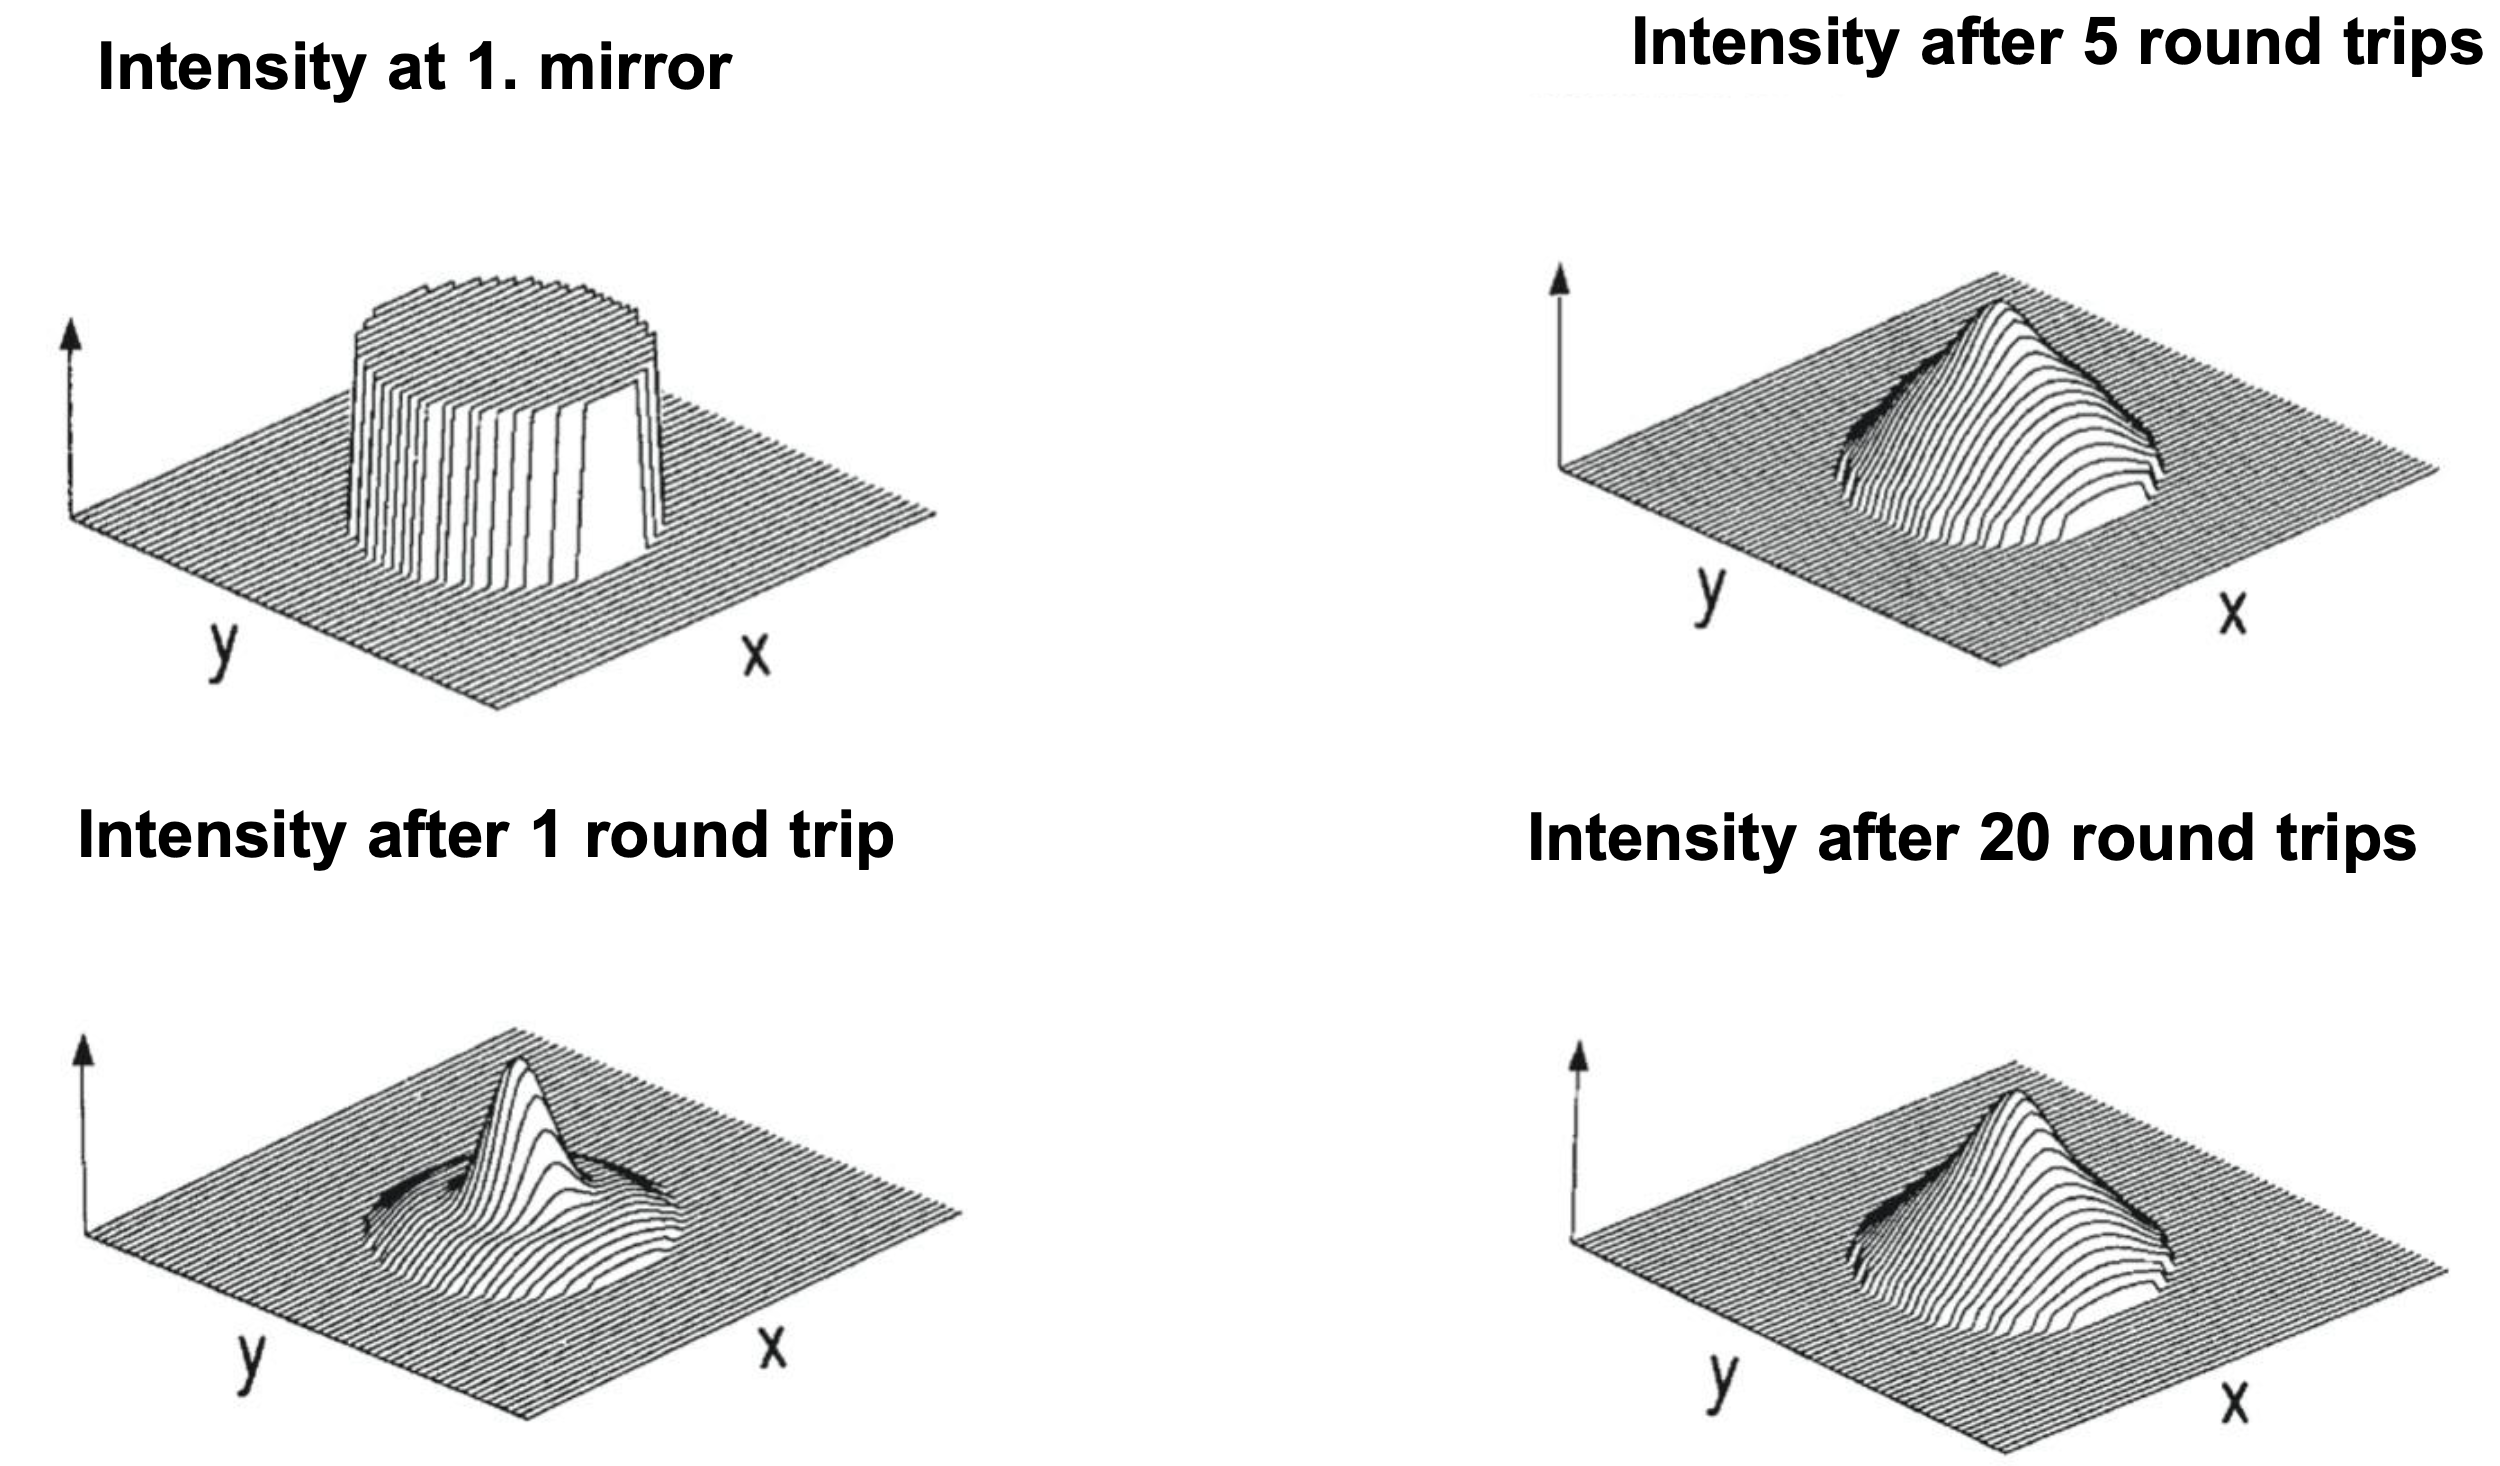
\includegraphics[width=0.5\textwidth]{slike/fbq1.png}
    \caption{Beam for $N_F=1$. \textit{Source:Lecture notes}}
    \label{fig:fbq1}
\end{figure}

A beam with $N_F=4$ has low diffraction losses and low improvement in beam quality - shown in figure \ref{fig:fbq2}.
\begin{figure}[h!]
    \centering
    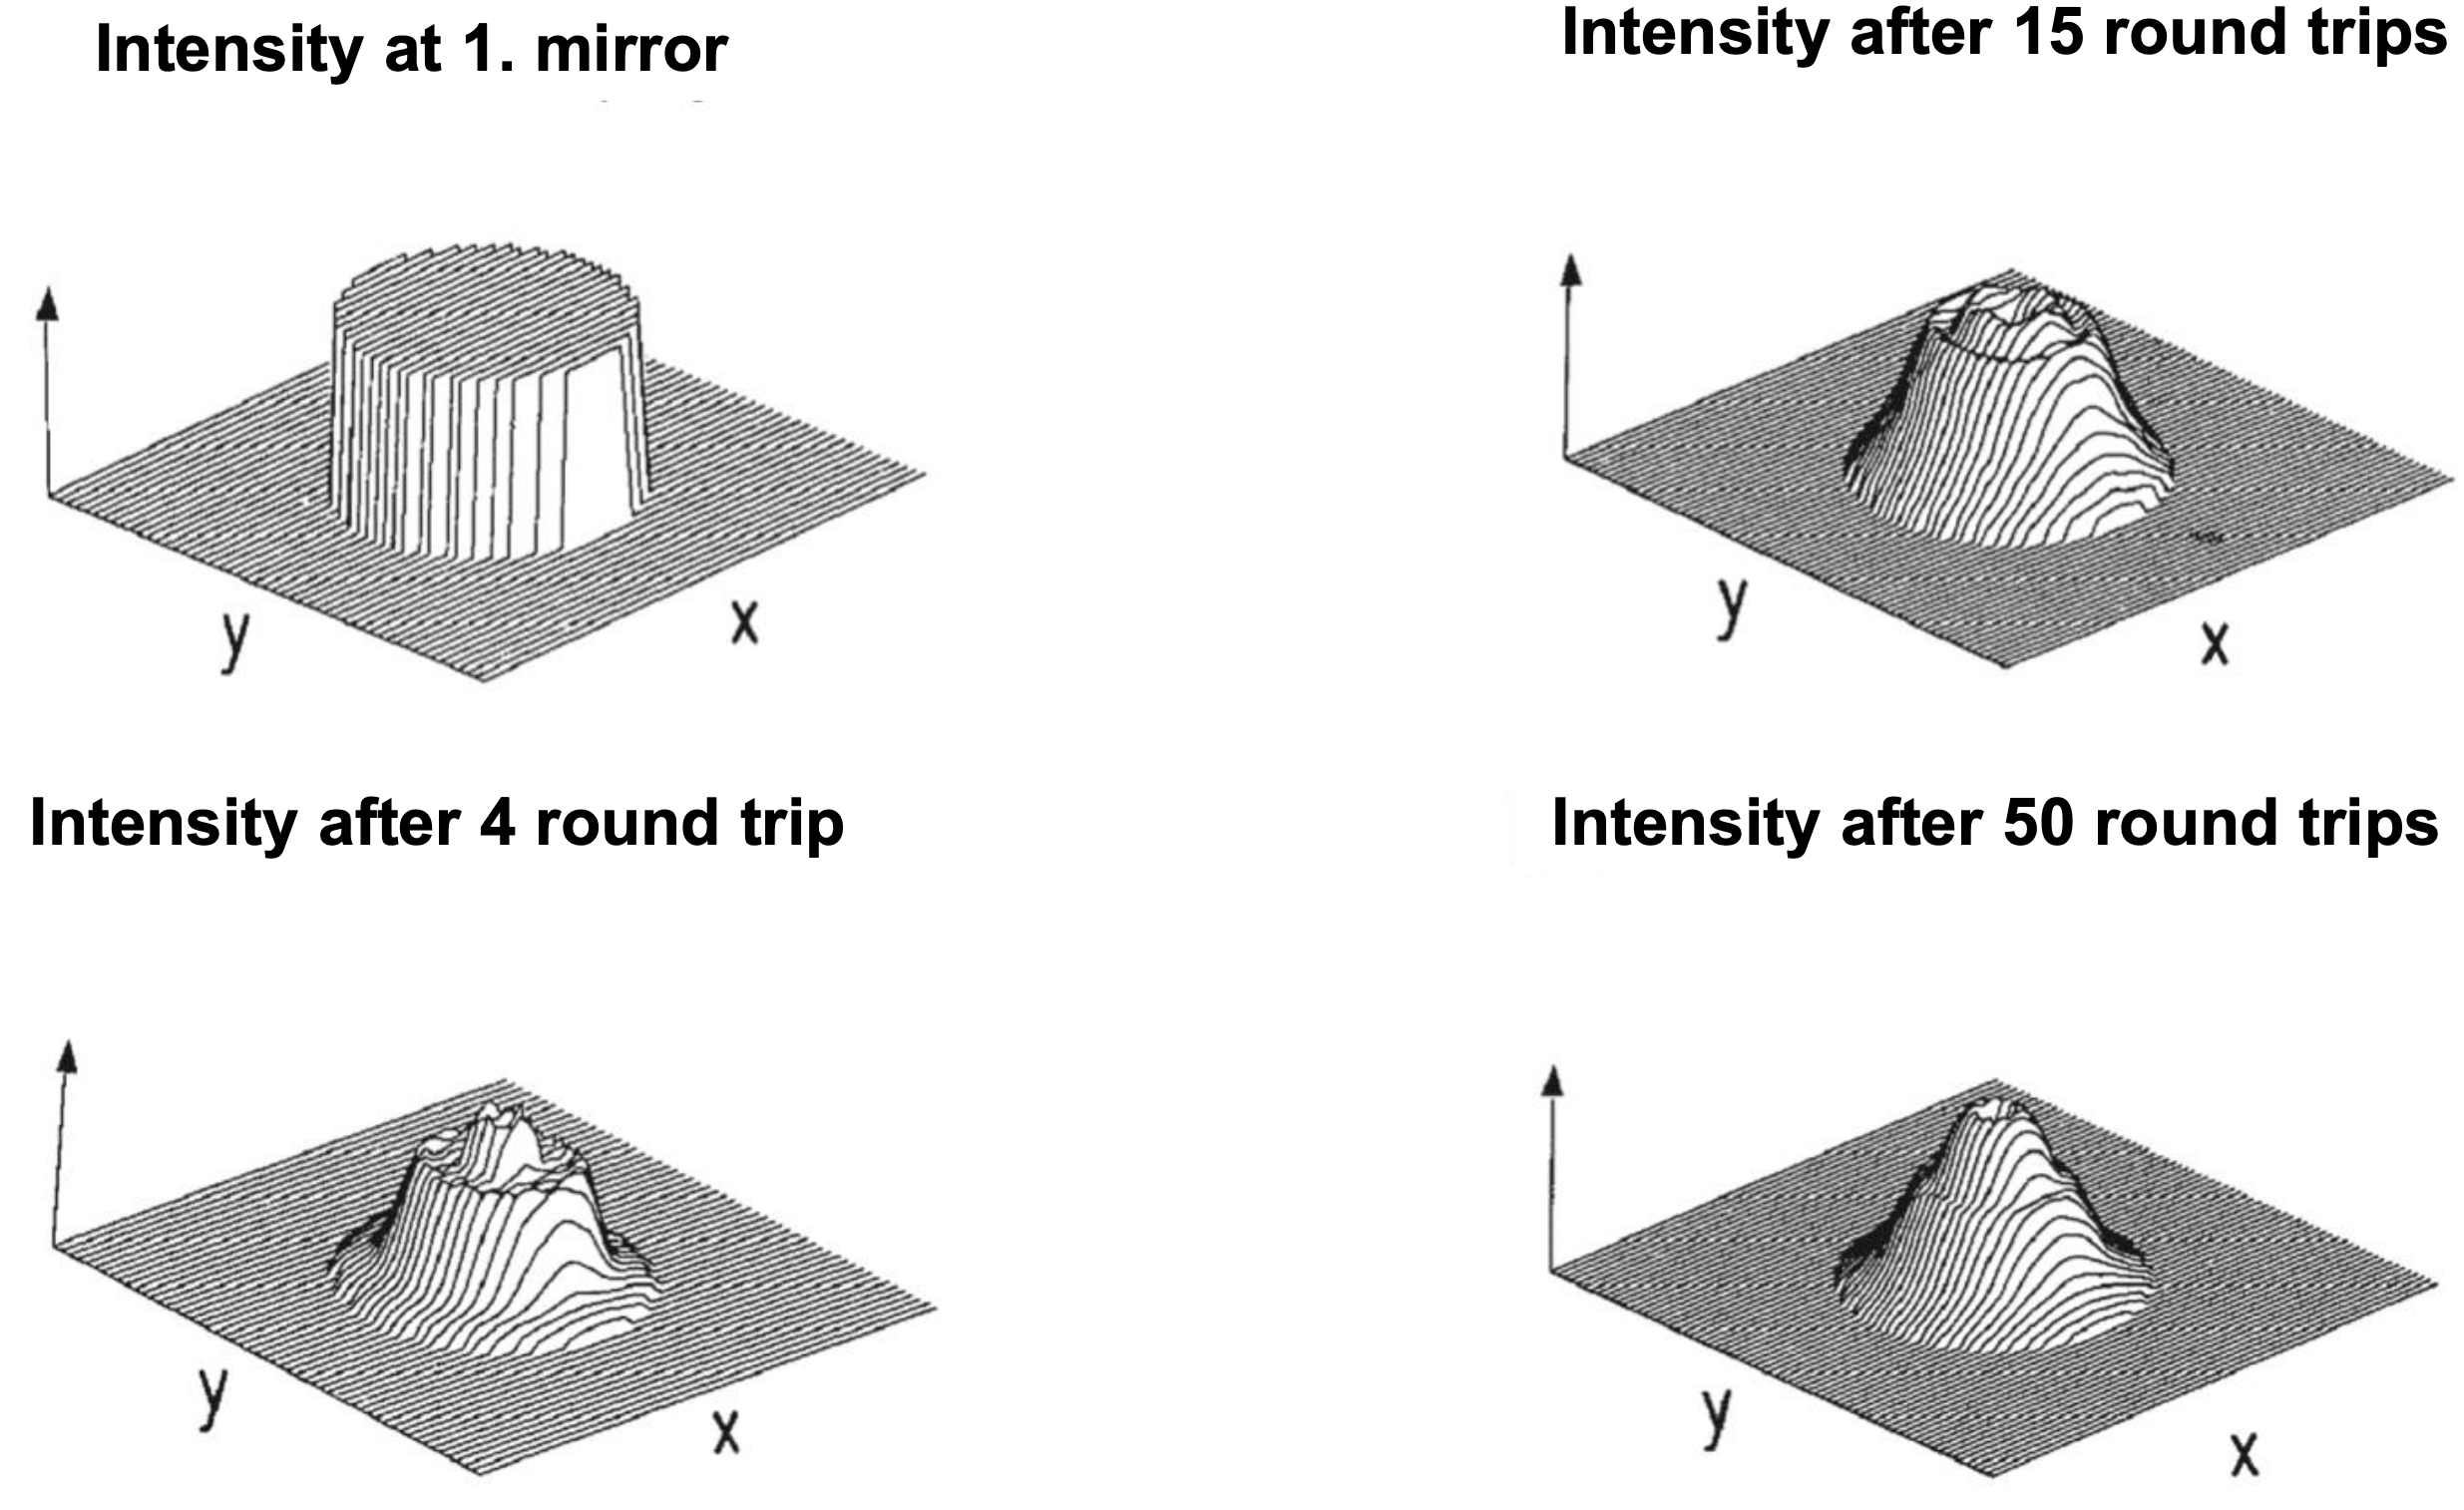
\includegraphics[width=0.5\textwidth]{slike/fbq4.png}
    \caption{Beam for $N_F=4$. \textit{Source:Lecture notes}}
    \label{fig:fbq2}
\end{figure}

\section{Multi Mode Operations}

In a stable resonator, stable beam trajectories satisfy the equation $R \cdot \vec{b} = \pm\vec{b}$.
Such beam must be an eigenstate of the resonator, in order to repeatedly pass through it. 

Laser active medium provides an intensity distribution $A_0 \cdot e^{-\frac{x^2}{2}}$.
Diffraction causes the profile to transform into a wave-vector distribution profile,
$\mathcal{F}(A_0 e^{-frac{x^2}{2}}) \rightarrow A_0 e^{-\frac{k^2}{2}}$, where $k$ is $x$ in angular space.

In the laser gain medium only certain waves gain energy, all waves loose energy due to
mirrors and other aperture-like components. (Main) Wave vector distribution is converted into
an intensity profile, equation \ref{eq:gdp1}.
\begin{equation}
    \mathcal{F} \left\{ A_0 e^{-\frac{k^2}{2}}\right\} \rightarrow A_0 e^{-\frac{x^2}{2}}
    \label{eq:gdp1}
\end{equation}
Such laser, with only one beam, has an EM-wave whose distribution is an eigenvector of a Fourier transform - equation \ref{eq:Item00}.
\begin{equation}
    I_{TEM_{00}} = I_0 exp \left( -2\frac{x^2+y^2}{w(z)^2}\right) = I_0 exp\left( -2 \frac{r^2}{w(z)^2} \right)
    \label{eq:Item00}
\end{equation}

\text{Such profile is called $TEM_{00}$}.

\subsection{Spatial hole burning}
When laser reaches population inversion in inhomogeneity, several \textbf{modes} can occur at the same time.

Figures $1.-4.$ shows the process of spatial hole burning. Population inversion is shown in picture $1.$,  Gaussian is excited first (picture $2.$) - centeral gain of the prifiles is reduced, but the 
outer area is mostly unused. In the population inversion in the outer area (picture $3.$) is high enough, the resonator can 
support more complex beam profile. Higher mode is excited (picture $4.$).

\begin{figure}[h!]
    \centering
    \includegraphics[width=0.65\textwidth]{slike/spatialholeburning.pdf}
    \caption{Spatial hole burning}
    \label{fig:shb}
\end{figure}
The spectral profile of new spectral shapes will not change as long as the new wavelength 
has the same losses and gain as the one before. 

\section{Transverse Electromagnetic Modes - TEM}
A \textbf{transverse mode} of electromagnetic radiation is an electromagnetic
field pattern of EM radiation in the plane perpendicular to the propagation direction.
Figure \ref{fig:tmpr} shows some possible modes in a passive resonator.
\begin{figure}[h!]
    \centering
    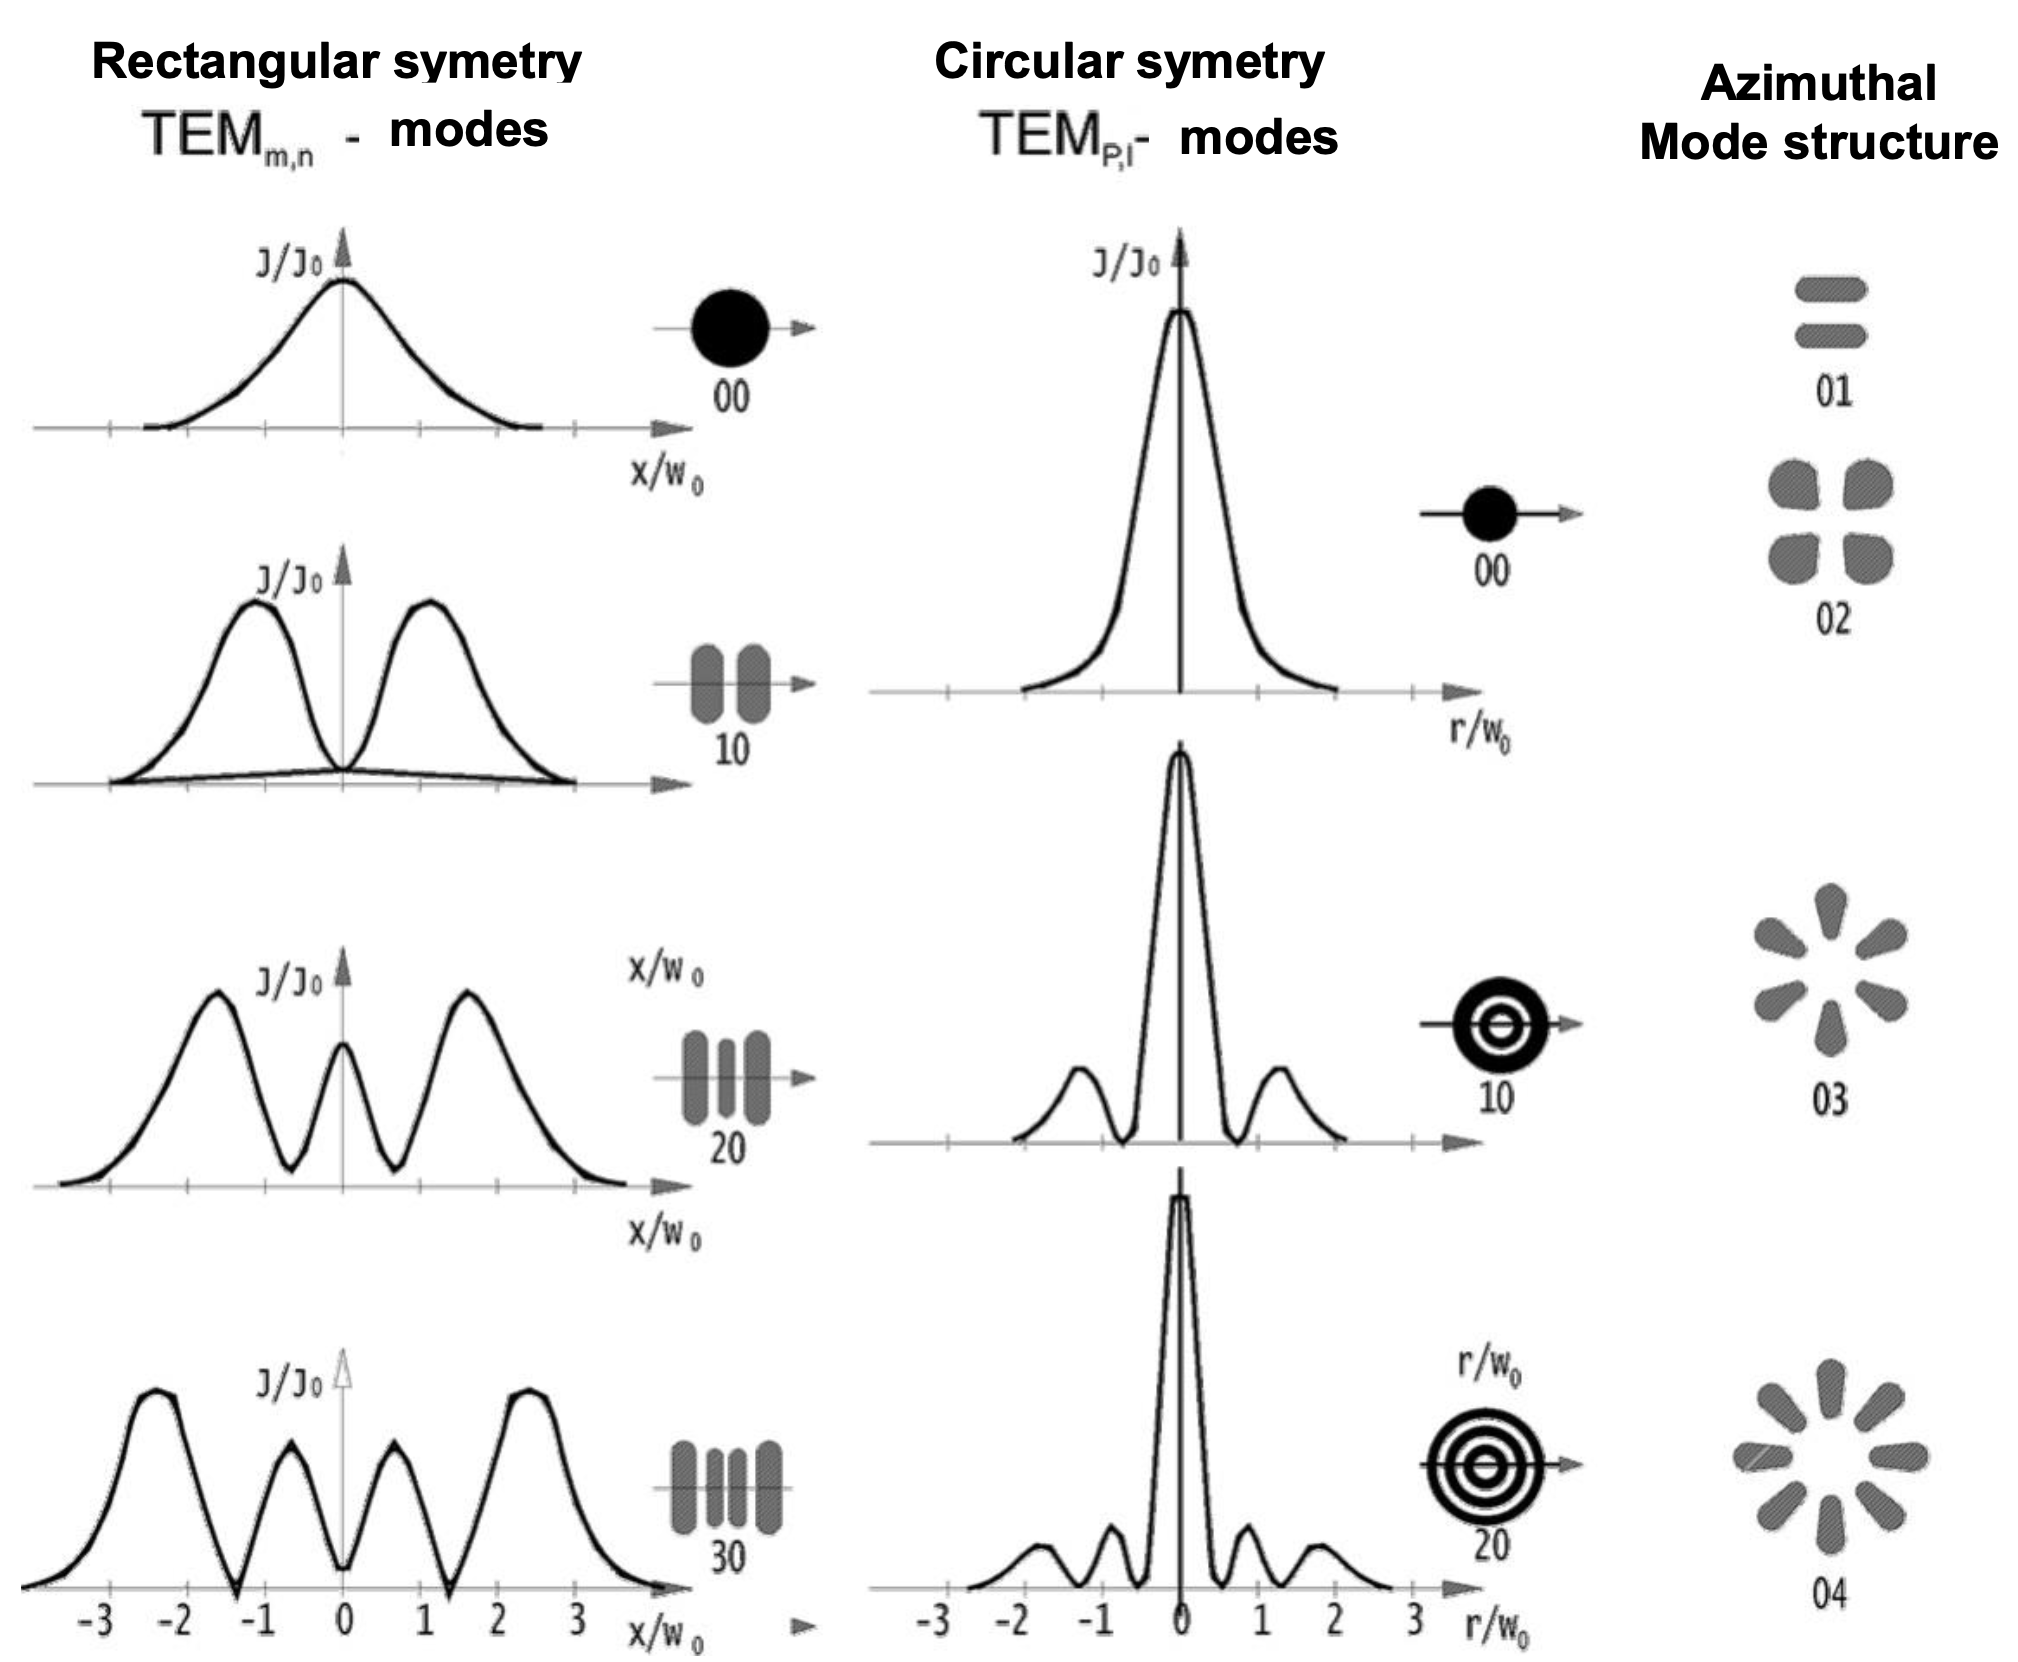
\includegraphics[width=0.5\textwidth]{slike/TransverseModes.png}
    \caption{Transverse modes of passive resonator.\\ \textit{Source: Lecture notes}}
    \label{fig:tmpr}
\end{figure}
Higher order $TEM$ can lead to complex polarization behaviour. In high power lasers several modes can overlap to create a hybrid mode.
If a laser emits more than one mode, it is called a multimode laser. A single mode laser emits mostly one or only one mode - $TEM_{00}$.
For applications that require good focusabillity we have to use a single mode laser.

Transverse modes are caused by path the light takes inside the resonator.
Actual path of the light ray is not equal to the distance between the mirrors. 


To reduce the amount of modes in a laser, we induce losses to higher order modes by placing a 
fixed or variable aperture inside the laser cavity.

\subsection{Circular symmetry}
In lasers, transverse modes are described as a combination of a \textbf{Gaussian beam} profile 
and a \textbf{Lagrange polynomial}. Modes are written as $TEM_{p,l}$, equation \ref{eq:temdef}.

\begin{equation}
    E_{p,l, \varphi} = E(0,z) \cdot exp\left( -\frac{r^2}{w(z)^2} \right) \cdot \left(\frac{\sqrt{2}r}{w(z)}\right)^l \cdot L^l_p \left(\frac{2r^2}{w(z)^2} \right) \begin{cases}
        cos(l\varphi)\\
        sin(l\varphi)
    \end{cases}
    \label{eq:temdef}
\end{equation}

$L^p_l$ is the \textbf{Lagrange polynomial}, $p$ is the degree of polynomial (number of zero crossings in radial direction) and $l$ is the number of zero crossing in $\varphi$ direction. 
Beam radios is given by $w$.

Figure \ref{fig:tmcr} shows shapes of different TEM.
\begin{figure}[h!]
    \centering
    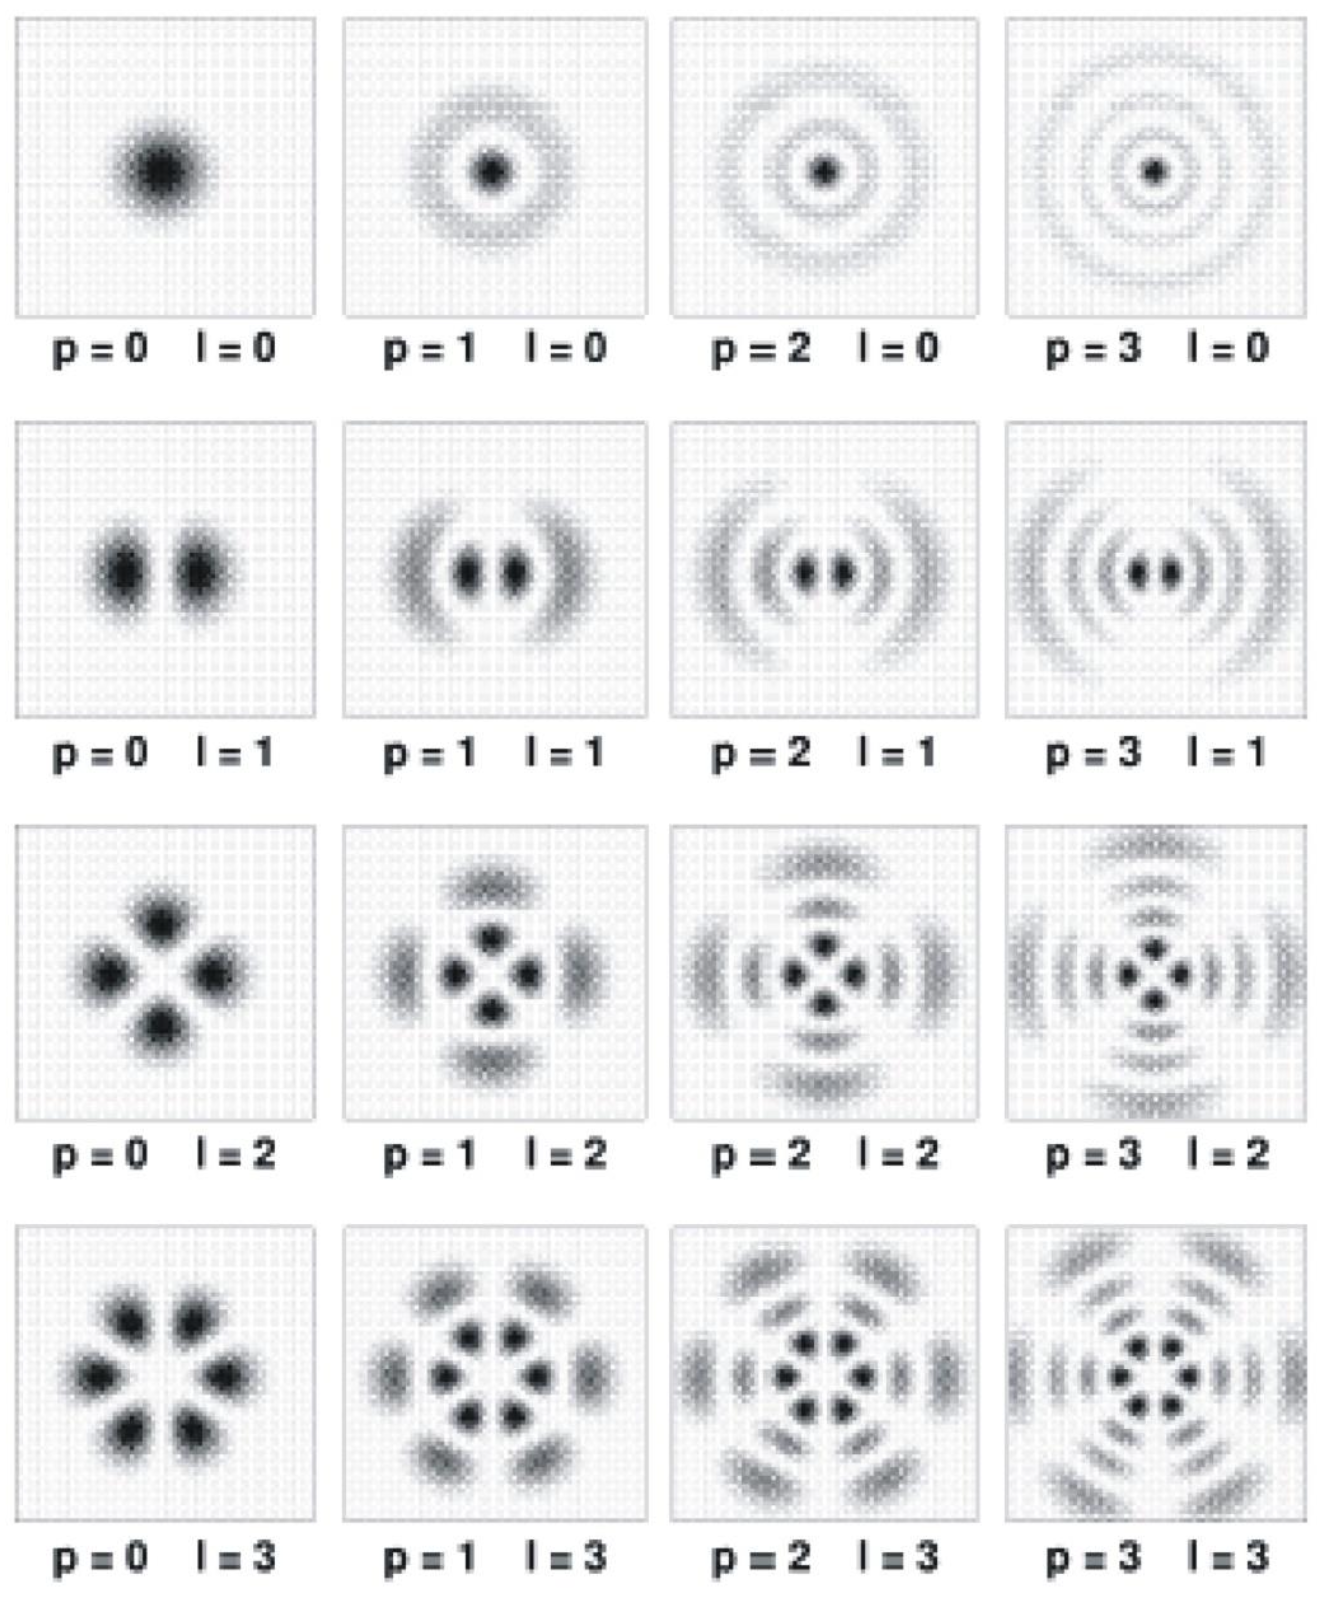
\includegraphics[width=0.3\textwidth]{slike/tmcr.png}
    \caption{Transverse mode structure in a circualr passive resonator.\\ \textit{Source: Lecture notes}}
    \label{fig:tmcr}
\end{figure}


\subsection{Rectangular symmetry}
%is profile equal to gauss and hermite polynomials.
For rectangular resonator symmetry, electric field is given by the equation \ref{eq:temrec}.
\begin{equation}
    E_{m,n} (x,y,z) = E(0,0,z) exp \left( -\frac{x^2+y^2}{w(z)^2} \right) \cdot H_m \left(\frac{\sqrt{2}x}{w(z)} \right) \cdot H_n \left(\frac{\sqrt{2}y}{w(z)} \right)
    \label{fig:temrec}
\end{equation}

Hermite polynomial $H_i$ has a degree - number of zero crossings - of $i$. Beam radius is equal to $w(z)$.
\begin{figure}[h!]
    \centering
    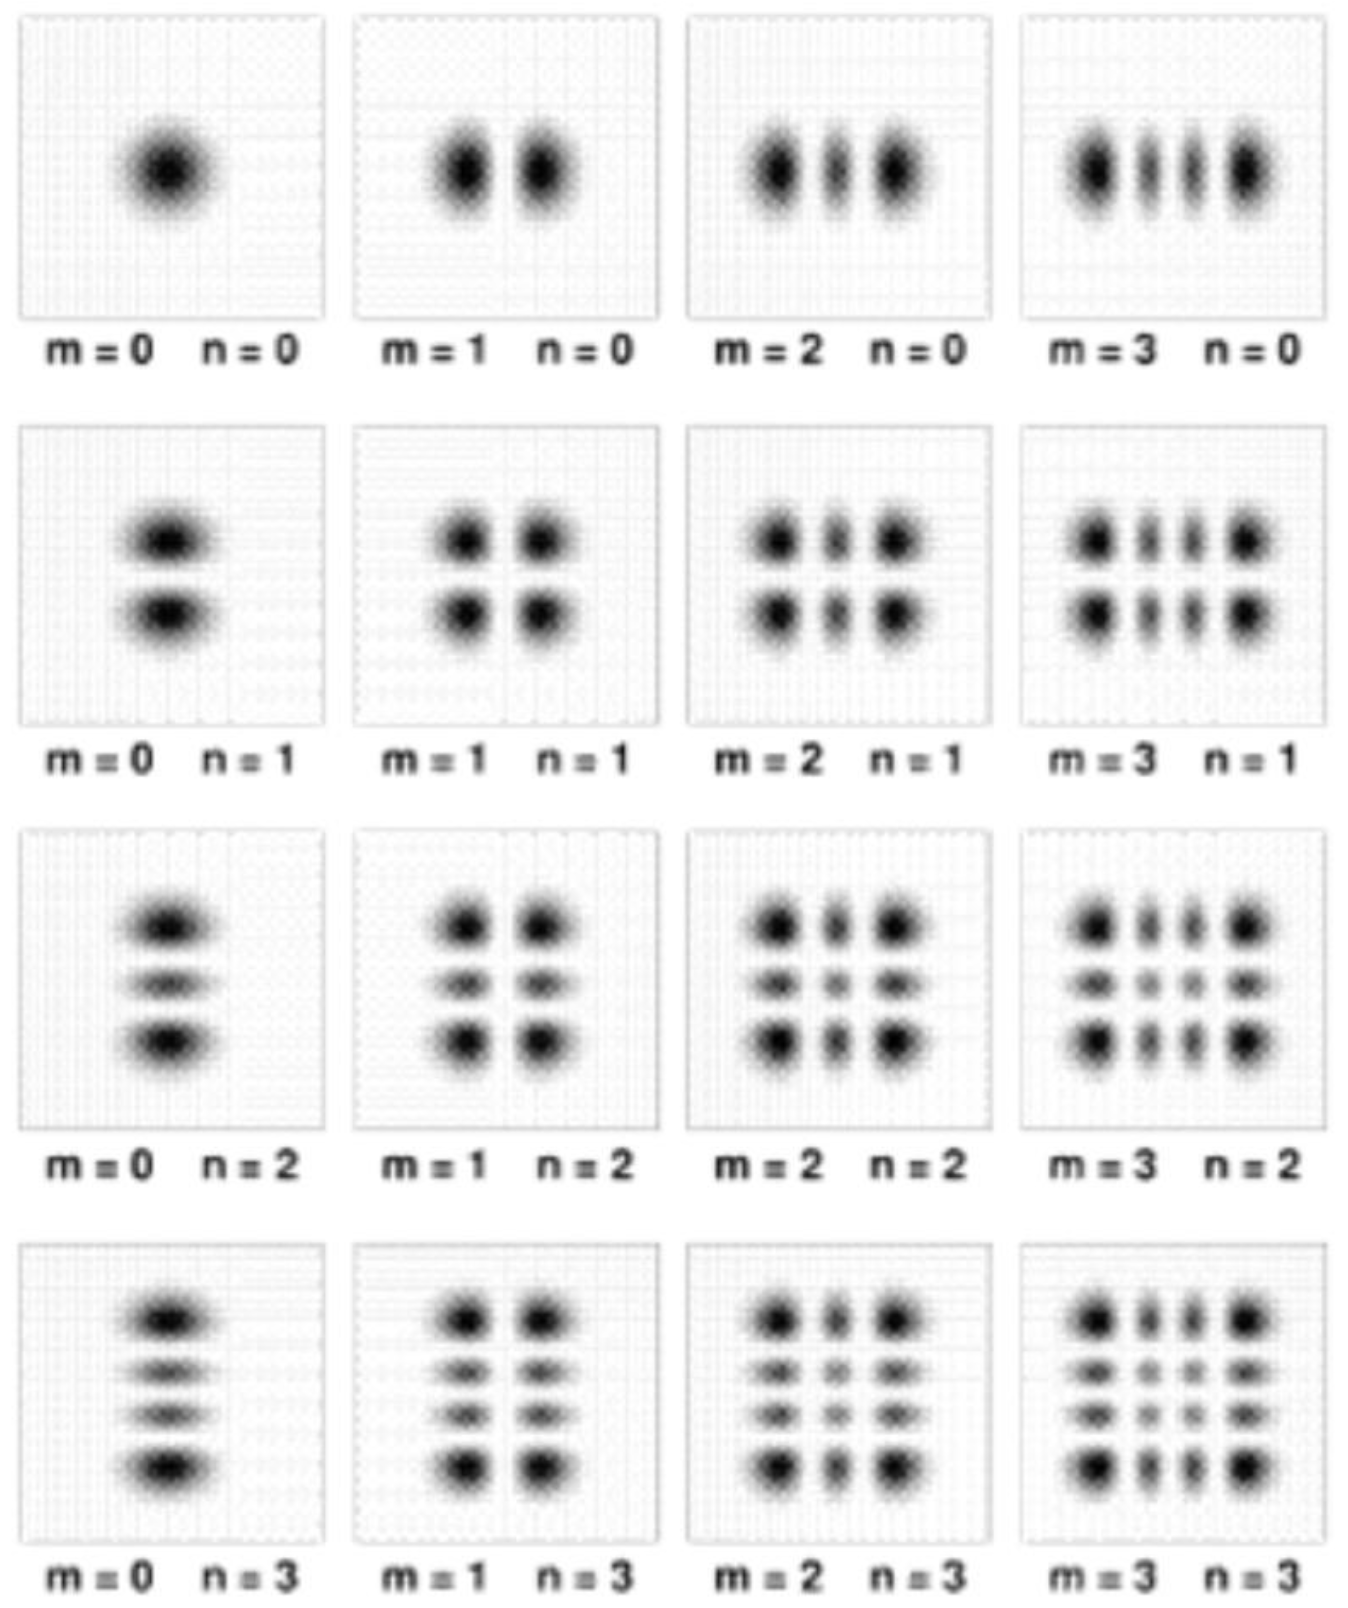
\includegraphics[width=0.3\textwidth]{slike/tmrr.png}
    \caption{Transverse mode structure in a rectangular passive resonator.\\ \textit{Source: Lecture notes}}
    \label{fig:tmrr}
\end{figure}




\newpage
\chapter{Beam Propagation}
\section{Gaussian beam}
Gaussian beam is an ideal beam used in optics to simplify calculations.

If we assume a Gaussian beam and no aperture, figure \ref{fig:gbna}.
\begin{figure}[h!]
    \centering
    \includegraphics[width=0.6\textwidth]{slike/gbna.pdf}
    \caption{Gaussian beam with no aperture}
    \label{fig:gbna}
\end{figure}

Electric field at aperture is $E(x) = \sqrt{I_0} e^{-\frac{x^2}{w_0^2}}$, inserting it 
into equation \ref{eq:gbe1} and solving for every possible $x'$ and $d$ gives us a \textbf{Gaussian beam}.
% lectures only say gives us .... next slide -> Gaussain beam

\begin{equation}
    E_{\sum}
    \label{eq:gbe1}(x',d) = \int_{-\infty}^{+\infty} \frac{E(x)}{1+ \sqrt{ (x'-x)^2 + d^2}} e^{|\vec{k}|\cdot \sqrt{(x'-x)^2 + d^2}-\omega t } dx
\end{equation}

Figure \ref{fig:gaussbeam} shows the parameters of the Gauss beam, symbols are explained in table \ref{tab:gaussbeam}.
\begin{figure}[h!]
    \centering
    \includegraphics[width=0.9\textwidth]{slike/gaus_beam.pdf}
    \caption{Gauss beam and parameters}
    \label{fig:gaussbeam}
\end{figure}

\begin{table}[h!]
    \centering
    \begin{tabular}{|c|c|c|}
        \hline
        Parameter& Definition & Formula \\
        \hline
        $w(z)$ & Beam radius at $z$ & $w(z) = w_0 \sqrt{1 + \frac{z^2}{z_R^2}}$\\
        $\theta$ & Divergence angle & $\Theta = \frac{\lambda}{\pi w_0}$ \\
        $w_0$ & Beam waist & $w_0 = \sqrt{\frac{z_R \lambda}{\pi}}$\\
        $z_0$, $z_R$ & Rayleigh length & $z_R = \frac{\pi w_0^2}{\lambda}$ \\
        $\sqrt{2}w_0$ & Beam waist @ $z_R$ & $\sqrt{2}w_0$ \\
        R(z) & Wavefront curvature & $R(z) = z [ 1 + (\frac{z_R}{z})^2]$ \\

        \hline
    \end{tabular}
    \caption{Gauss beam parameters}
    \label{tab:gaussbeam}

\end{table}
\subsection{Parameters}

\subsubsection{Rayleigh length and beam waist}
\textbf{Beam waist} $w_0$ is the smallest radius of the beam - "focal spot". Laser intensity in this spot 
is the highest. Equation \ref{eq:inte} shows the strength of electric field at distance $x$.

\begin{equation}
    E(x,z) = \sqrt{I_0} e^{-\frac{x^2}{w_0^2}}
    \label{eq:inte}
\end{equation}
%z je argument funk. ni pa uporabljen?


\textbf{Rayleigh length} $z_R$ is the distance from the beam waist at which the intensity is halved.
It is calculated by equation \ref{eq:zR}.
\begin{equation}
    z_R = \frac{\pi w_0^2}{\lambda}
    \label{eq:zR}
\end{equation}

Rayleigh length is important for processing of rough surfaces because the beam diameter stays relatively  \textbf{constant and small}.

Beam radius depends on Rayleigh length and waist $w_0$, diameter $w(z)$ is calculated by \ref{eq:w}.
\begin{equation}
    w(z) = w_0 \sqrt{1 + \frac{z^2}{z_R^2}}
    \label{eq:w}
\end{equation} 
Beam power is equal to the integral of intensity over area given by $w$ - equation \ref{eq:beampower}.
\begin{equation}
    P_L(z) = \int_{0}^{\infty} I(r,z) \cdot 2 \pi r dr = 2\pi I_0(z) \int_{0}^{\infty}r e^{-\frac{2r^2}{w(z)^2}} dr = \frac{\pi}{2} w(z)^2 I_0(z)
    \label{eq:beampower} 
\end{equation}
If we assume energy conservation for any distance - equation \ref{eq:bp2}.
\begin{equation}
    P_L(z) = \frac{\pi}{2} w(z)^2 I_0(z) = \frac{\pi}{2} w(z)^2 I_0(z=0) \rightarrow I_0(z)=\frac{w_0^2}{w(z)^2} I_0(z=0)
    \label{eq:bp2}
\end{equation}
Power is \textbf{constant}, intensity changes. 

\subsubsection{ Divergence angle}
In the far field, where $z >> z_R$, we can simplify equation \ref{eq:w} to equation \ref{eq:ffw}.
\begin{equation}
    w(z >> z_R) =w_0 \sqrt{1 + \frac{z^2}{z_R^2}} \approx w_0 \frac{z}{z_R}
    \label{eq:ffw}
\end{equation}
Beam radius increases linearly, when $z >> z_R$, divergence in the far field is \ref{eq:ffd}.
\begin{equation}
    \theta = \underset{z >> z_R}{lim} \frac{w(z)}{z} = \frac{w_0}{z_R} = \frac{\lambda}{\pi w_0}
    \label{eq:ffd}
\end{equation}

Beam parameter product is:  $\theta w_0 = \frac{\lambda}{\pi} = const$

\textit{Note: The smaller the beam waist diameter the bigger the divergence (and vice versa).}


\section{Beam size}
Beam can be measured at any point of its height. In experiments the most convenient measurments 
height is at \textbf{half maximum}, this is called \textbf{Full Width Half Maximum}.
For mathematical operations, height of $\frac{1}{e^2}$ is used, which is 13.5\% of the peak.
Figure \ref{fig:beamFWHM} shows FWHM.
\begin{figure}[h!]
    \centering
    \includegraphics[width=0.5\textwidth]{slike/fwhm.pdf}
    \caption{FWHM}
    \label{fig:beamFWHM}
\end{figure}

For a rotationally symmetric Gaussian beam - $TEM_{00}$, there is a linear relationship 
between FWHM and beam radius - $FWHM = \sqrt{2 ln(2)}w(z) = 1.177 w(z)$.

\subsection{Higher order TEM}

Figure \ref{fig:hobtem} shows the Gaussian beam for higher order TEM. 
Symmetric beam can be radial or cartesian. 
Cartesian symmetry:
\begin{gather}
    w_{m,n} = w_{00} \sqrt{2s + 1}\\
    \Theta_{m,n} = \Theta_{00} \sqrt{2s + 1}
\end{gather} where $s = m,n$. For a cartesian system each direction is evaluated on its own.

% is m = n = s?
For radial symmetry:
\begin{gather}
    w_{p,l} = w_{00} \sqrt{2p + l + 1} \\
    \Theta_{p,l} = \Theta_{00} \sqrt{2p + l + 1}
\end{gather}

\begin{figure}[h!]
    \centering
    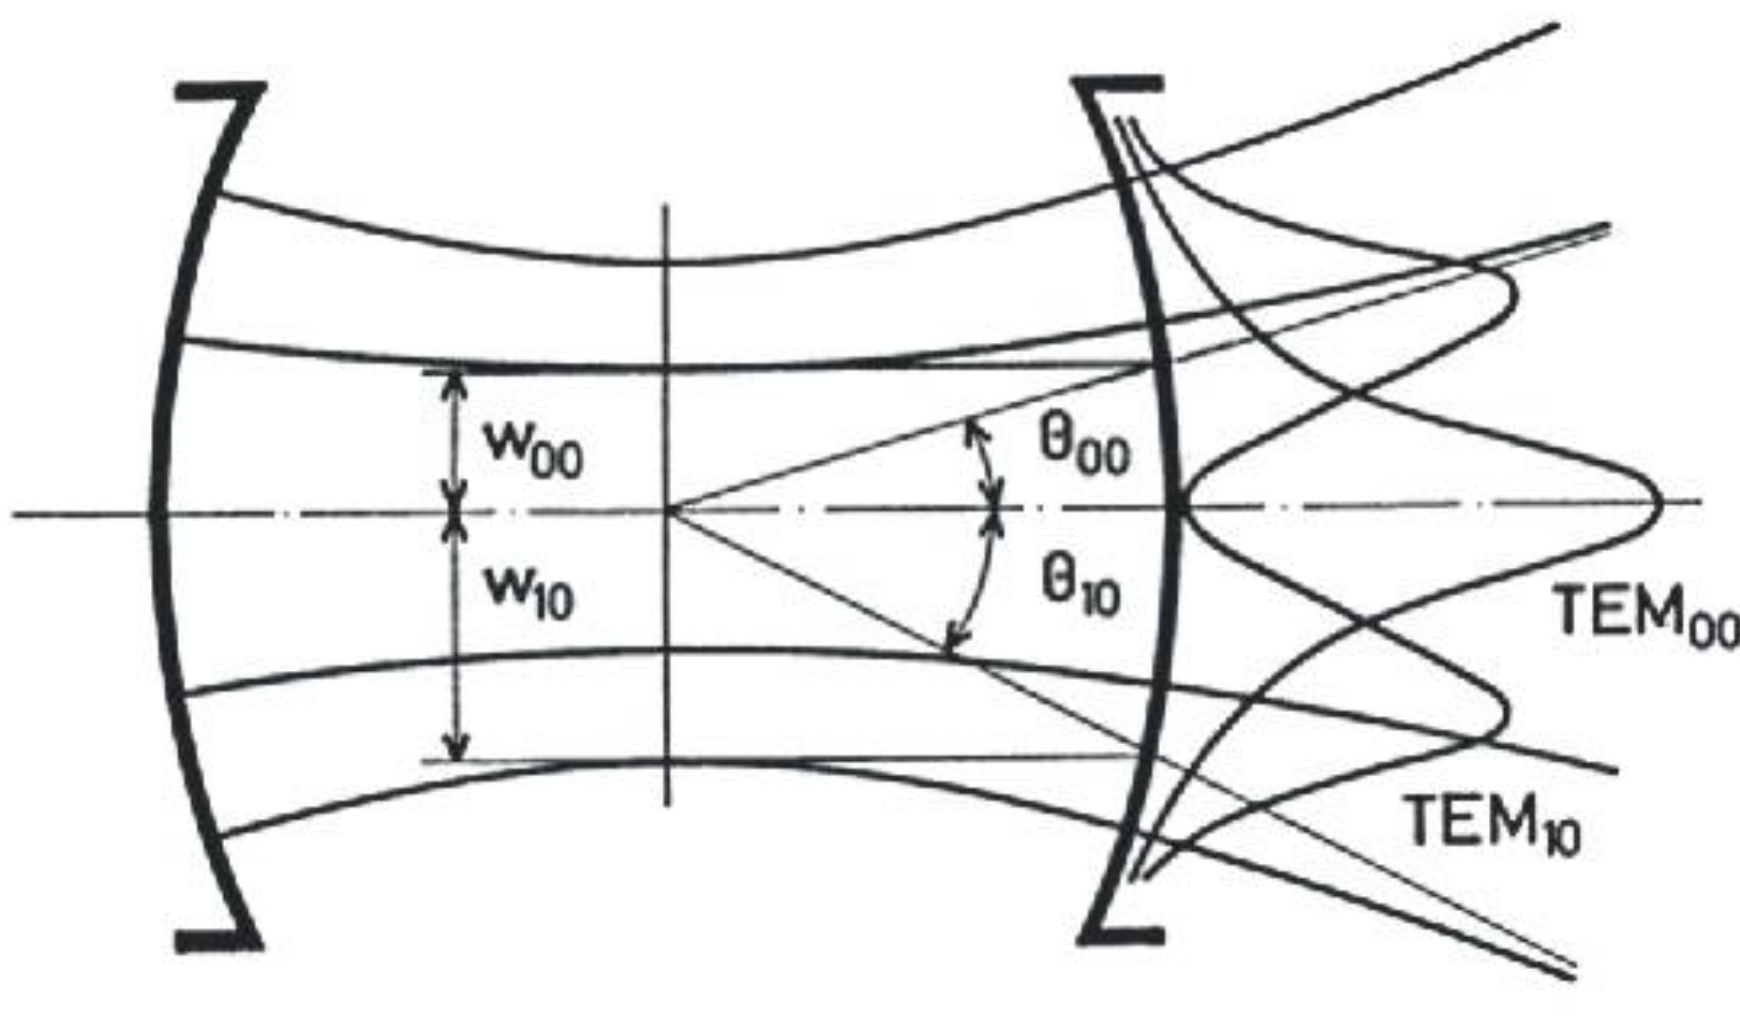
\includegraphics[width=0.5\textwidth]{slike/hobtem.png}
    \caption{Higher order TEM Gauss beam. \textit{Source: Lecture notes} }
    \label{fig:hobtem}
\end{figure}
 
Beam radius and divergence angle increases by a factor given by the mode structure.\\
\textbf{Conclusions}:
\begin{itemize}
    \item Focal spots for higher order modes are larger than for $TEM_{00}$ mode
    \item Higher order modes diverge faster than $TEM_{00}$ mode
    \item Higher order modes diverge differently
\end{itemize}

\section{Beam quality}
Beam propagation is simplified with a \textbf{beam quality factor} $M^2$.
Equation \ref{eq:M2} shows the definition.
\begin{equation}
    M^2 = \frac{(\Theta w)_{real}}{(\Theta_0 w_0)_{Gauss}}
    \label{eq:M2}
\end{equation}

For a Gauss beam whose  $M^2 = 1$ beam parameter product (BPP) is the smallest possible. 
All real beams have $1 < M^2 $. Ideal optical elements do not change the beam quality factor. 

Higher bam quality means:
\begin{itemize}
    \item Smaller focus diameter $\rightarrow$ higher intensity, lower divergence, better quality \dots
    \item Longer working distance $\rightarrow$ increased process stability, reduced risk for damaging optical components \dots
    \item Smaller optics $\rightarrow$ cheaper, more efficient cooling \dots
\end{itemize}

\textit{Note: in calculations $M^2$ is always multiplied with $\lambda$}.

\section{Focusing of Gaussian beams}

Due to optical aberrations/imperfections and diffraction, limited spot sizes are 
not achievable. Both increase the $M^2$ and the beam parameter product.
Equation \ref{eq:rbeam} shows the waist size accounting for imperfections.

\begin{equation}
    w_f = \textcolor{black}{\frac{2\lambda}{\pi} \cdot \frac{f}{D} \cdot M^2} + \textcolor{blue}{ C_L \cdot \frac{D^3}{f^2} }
    \label{eq:rbeam}
\end{equation}
Where $D$ is the laser beam diameter.  Figure \ref{fig:saber} show the spherical aberration, which also increases $M^2$, coloured blue in equation \ref{eq:rbeam}.


\begin{figure}[h!]
    \centering
    \includegraphics[width=0.3\textwidth]{slike/saberation.pdf}
    \caption{Spherical aberration}
    \label{fig:saber}
\end{figure}

If the following beam properties:
\begin{itemize}
    \item Short wavelength
    \item Short focal length
    \item Large beam diameter
    \item Using well suited lens combinations
\end{itemize}
Are present, we can simplify the equation \ref{eq:rbeam} to $w_f = \textcolor{black}{\frac{2\lambda}{\pi} \cdot \frac{f}{D} \cdot 1}$, as the other parameters are negligible.

\section{Gaussian beam propagation}

Figure \ref{fig:gbp} shows the effect a lens has on a  plane wave beam.
\begin{figure}[h!]
    \centering
    \includegraphics[width=0.5\textwidth]{slike/gaussbeampropagation.pdf}
    \caption{Gauss beam propagation}
    \label{fig:gbp}
\end{figure}

Lens imposes a curvature on the beam, equation \ref{eq:Rlns}. Change in curvature imposed by the propagation in free space
is given by equation \ref{eq:Rfree}
\begin{equation}
    R_{new} = R_{old} + f
    \label{eq:Rlns}
\end{equation}
\begin{equation}
    R(z) = z (1 + \frac{z_R^2}{z^2})
    \label{eq:Rfree}
\end{equation}
Combining equations leads to equation \ref{eq:Rnew}.
\begin{equation}
    \frac{1}{R_{new}} = \frac{1}{z (1 + \frac{z_R^2}{z^2})} + \frac{1}{f_{@z}}
    \label{eq:Rnew}
\end{equation}

To separate curvature and beam size, we use \textit{complex numbers}.

\subsection{Complex q-parameters}
Complex parameter q is defined by equation \ref{eq:qparm}.
\begin{equation}
    \frac{1}{q(z)} = \frac{1}{(z + \frac{z_R^2}{z})} - i \frac{1}{z^2 + z_R^2} = \frac{1}{R(z)} - i \frac{\lambda}{\pi w(z)^2}
    \label{eq:qparm}
\end{equation}
Which is equal to \ref{eq:qinv}.
\begin{equation}
    q(z) = \frac{\frac{1}{R}}{R^2 + (\frac{\lambda}{\pi w^2})^2} + i \frac{\frac{\lambda}{\pi w^2}}{R^2 + (\frac{\lambda}{\pi w^2})^2}
    \label{eq:qinv}
\end{equation}

New free space propagation equation is $q(z) = z + i z_R$. \textbf{Real part} of $\frac{1}{q}$ is the \textbf{curvature}, \textbf{imaginary part} is the \textbf{site of beam} at z.

\subsubsection{Q-parameter at lens}
Real part of $\frac{1}{q}$ is equal to zero. Lens changes the curvature to the radius of $f$. New real 
part is therefore $\frac{1}{f}$. If the beam already has a curvature before the lens, 
the lens will make curvature even smaller, according to equation \ref{eq:qlens}.
\begin{equation}
    \frac{1}{q_{out}} = 0 + i \frac{1}{z_R} + \frac{1}{f} = \frac{1}{q_{in}} + \frac{1}{f}
    \label{eq:qlens}
\end{equation}

At position $z=0$ the curvature is infinite, q parameters are equal to:
\begin{equation}
    \frac{1}{q(z=0)} = 0 + i \frac{1}{z_R}
\end{equation}

We can also use \textit{q parameters} with the ABCD matrix computation, $q_f$ is equal to
\begin{gather}
    q_f = \frac{A q_i + B}{C q_i + D} \\
    \frac{1}{q_f} = \frac{C + D/q_i}{A + B/q_i}
\end{gather}

\newpage
\chapter{Light Matter Interaction}
\section{Basic of laser processing} %410

When dealing with laser processing, we will make the assumptions of steady state and spherical heat distribution.

\subsection{Heat conduction}
Heat conduction through a spherical shell is given by \ref{eq:hcss}.
\begin{equation}
    Q = -k (4 \pi r^2)\frac{dT}{dr} \rightarrow \frac{Q}{4\pi k}\int_{r1}^{r2} \frac{1}{r^2} dr = -\int_{T_1}^{T_2} dt 
    \rightarrow T_1 - T_2 = \frac{Q}{4 \pi k} \left(\frac{1}{r_1} - \frac{1}{r_2} \right)
    \label{eq:hcss}
\end{equation}
We assume that the material is infinitely thick $r_2 \rightarrow \infty$ and that 
room/environment  temperature $T_2 = T_{env} = 25^{\circ} C$. Thermal conductivity is
given by $k$. Heat flow due to conduction is given by equation \ref{eq:qmat}.
\begin{equation}
    Q_{MAT} = 2\pi k (T-T_0) \cdot r_{HAZ}
    \label{eq:qmat}
\end{equation}

\subsection{Radiative energy losses}

\textbf{Black body} is an idealized physical body that absorbs all the incident electromagnetic radiation. 
It has perfect absorptivity at all wavelengths, it is the best possible emitter of thermal radiation - it radiates in a characteristic continuous 
spectrum that depends on its temperature. Figure \ref{fig:bb}
\begin{figure}[h!]
    \centering
    \includegraphics[width=0.3\textwidth]{slike/blackbody.pdf}
    \caption{Black body}
    \label{fig:bb}
\end{figure}
Planck's Law determines the thermal equilibrium T, equation \ref{eq:plaw}.
\begin{equation}
    \rho(\nu, T) = \frac{2 h \nu^3}{c^2} \frac{1}{e^{\frac{h\nu}{k_B T}-1}}
    \label{eq:plaw}
\end{equation}
Where $\rho$ is the spectral radiance at the density of frequency $\nu$ radiation per unit frequency,
$h$ is the \textit{Planck constant}, $k_B$ is he Boltzmann constant, $T$ the absolute temperature of the body.

Power emitted by thermal radiation is equal to given by \textbf{Stefan-Boltzmann law}, equation \ref{eq:sbl}.
\begin{equation}
    P(T) = \varepsilon \int_{v=0}^{\infty} \int_{\Omega = 0}^{2\pi} \int_{A} \rho(\nu,T)\, dA\, d\Omega \, d\nu = \varepsilon \sigma A T^4
    \label{eq:sbl}
\end{equation}
Where $\varepsilon$ is the emission coefficient, $0 \le \varepsilon \le 1$, $A$ is the emitting area,
$\Omega$ the emitting angle and $\sigma$ is the \textit{Stefan-Boltzmann constant}, which is equal to 
$\sigma = 5.67 \times 10^{-8} \frac{W}{m^2 K^4}$. 
For a small body at temperature $T_1$ in a large room with $T_2$:
\begin{equation}
    p \approx \varepsilon \sigma A (T_{1}^4 - T_2^{4})
\end{equation}
The relation is \textbf{nonlinear}. Compared to \textbf{conductive heat losses}, the radiation losses are \textbf{small}.

\subsection{Evaporative and Convective losses}
\textbf{Evaporative losses} are $P_V = H_V \frac{dn}{dt}$, where $n$ is the amount of substance in mol, $H_V$ is the evaporation enthalpy.
\textbf{Heat required for melting} $P_M = H_M \frac{dn}{dt}$ where $H_M$ is fusion enthalpy.

\textbf{Heat required for heating} is $P_H = c_H \Delta T \frac{dn}{dt}$, where $c_H$ is the heat capacity and $\Delta T$ is the temperature difference.


\section{Light Matter Interaction}
Light-matter interaction dependencies:
\begin{itemize}
    \item Wavelength
    \item Material (structure)
    \item Pulse Duration
    \item Intensity
    \item Coupling mechanisms
    \item Rate of energy input
\end{itemize}

Coupling mechanisms of light and material are \textbf{direct absorption} and \textbf{plasma interaction}.
One of material properties is the band structure of solids.  A high amount of atoms makes it hard to distinguish 
between the energy levels  - we get valence bands. Shown on figure \ref{fig:vbonds}.
\begin{figure}[h!]
    \centering
    \includegraphics[width=0.5\textwidth]{slike/bandform.pdf}
    \caption{Line bandwidth}
    \label{fig:vbonds}
\end{figure}

\subsection{Band Structure of Solids}
Different material types - \textit{metals, semiconductors, insulators} - have different sized bandgaps. 
Band structure determines which type conductive property a material has.  Figure \ref{fig:bandsolids} shows the band 
structure of different materials.

\begin{figure}[h!]
    \centering
    \includegraphics[width=0.75\textwidth]{slike/mat_bandgap.pdf}
    \caption{Band structure of solids}
    \label{fig:bandsolids}
\end{figure}

\textbf{Metals} have \textit{overlapping }  valence and conduction band. 
\textbf{Semiconductors} have a small bandgap, \textbf{dielectrics} have a large bandgap.

\subsection{Coupling mechanisms}
Photons can interact with material's valence band by \textbf{plasma interaction} or \textbf{direct absorption}.

Directly absorbed photons change the molecule dipole moment. They interact with bound electrons  in the valence band.

With plasma interaction photons are absorbed or reflected. Photons interact with 
free of quasi-free electrons in the conduction band.

Absorption can be \textit{linear or nonlinear}. Ionization is either \textit{thermal or nonlinear}.
% is thermal ionization linear? is nonlinear ionization thermal?

\subsubsection{Linear absorption}
Linear absorption  can be either:
\begin{itemize}
    \item Spontaneous $\rightarrow$ fluorescence
    \item Radiationless relaxation  $\rightarrow$ heat input into material, most common interaction (even for optical transitions)
    \item Lattice vibrations \pd can be excited in almost all materials, with phonon energies $\le 0.1 \, eV$. Directly excited by infrared and microwave-range photons.
\end{itemize}

End result of linear absorption - heating is reshaping (by temperature gradient effect), melting/liquification, evaporation or sublimation.
If heating has a high rate, we can generate plasma. Figure \ref{fig:linabsor} shows linear absorption.
\begin{figure}[h!]
    \centering
    \includegraphics[width=0.5\textwidth]{slike/linabs.pdf}
    \caption{Linear absorption}
    \label{fig:linabsor}
\end{figure} 


\subsection{Nonlinear absorption}

Nonlinear absorption ionizes multiple photons at the same time, this results in immediate plasma generation.
All further interactions are the same as with plasma. 
Figure \ref{fig:nonlinabs} show nonlinear absorption of four photons.
\begin{figure}[h!]
    \centering
    \includegraphics[width=0.35\textwidth]{slike/nonlinabs.pdf}
    \caption{Nonlinear absorption}
    \label{fig:nonlinabs}
\end{figure}

\section{Thermal ionization}
Thermal ionization is a process in which electrons are emitted from a surface due to heating. 
Population density in this surface follow the \textit{Boltzmann distribution}. Figure \ref{fig:tion} shows the
valence bands and population distribution. 

\begin{figure}[h!]
    \centering
    \begin{subfigure}{0.35\textwidth}
        \includegraphics[scale=0.75]{slike/thermion.pdf}
        \caption{Valence bands and transmission. \textit{Source: Lecture notes.}}
    \end{subfigure}
    \begin{subfigure}{0.35\textwidth}
        \includegraphics[scale=0.6]{slike/therionpop.pdf}
        \caption{Thermal ionization population}
    \end{subfigure}
\end{figure}

\section{Light-Plasma interaction}

EM-wave and plasma interact - plasma reflects the EM-wave. Oscillation frequency of EM-Wave limits the distance the electron can travel. When an ion is close to
by the electron the displacement of electron compared to ion causes a change in Coulomb force between the electron and ion.
Electric field of the electron-ion pair is eh exact opposite ($\pi$ shifted) to the input EM-wave. 
Incoming EM-wave or photon is effectively reflected.

If we consider \textbf{low density plasma}, in which electrons are far from ions, the dipole moment does not change its direction.
Very weak opposite EM-wave is generated - plasma has deep reflectivity and the EM-wave can reach 
deep into the plasma.
EM-wave can penetrate plasma when it has a higher frequency than oscillating electrons at ions or the plasma is low density.

Reflection capability of plasma is given by the plasma frequency - equation \ref{eq:pfe}.
\begin{equation}
    \omega_{pe} = \sqrt{\frac{n_e e^2}{m \varepsilon_0}}
    \label{eq:pfe}
\end{equation}
Where $m$ is the mass of electrons, $\varepsilon_0$ is the vacuum permeability, $e$ the charge of electrons and $n_e$ the density of free electrons.
Figure \ref{fig:rhoplas} shows the different plasma densities. 
\begin{figure}[h!]
    \centering
    \includegraphics[width=0.5\textwidth]{slike/plasmadensity.pdf}
    \caption{High and Low density plasma}
    \label{fig:rhoplas}
\end{figure}


\section{Plasma heating}

\subsection{Joule or Coulomb heating}

Electrons are accelerated by \textbf{electric filed}.  They gain kinetic energy, as long as the
E-filed does not switch direction. If electron hits another particle during this phase, energy can transfer from 
EM-wave into plasma - inelastic scattering. Is particles do not collide during the first half of EM-wave electrons will be decelerated in the next half-wave - possibility of
energy transfer and no plasma heating.

This effect is similar to current in a wire - resistance heating.

\subsection{Inverse Bremsstrahlung}

Electrons are accelerated by \textbf{inelastic scattering of high energy photons on electrons.}
The gain of kinetic energy of electrons depends on the number of inelastically scattered photons. Such photons must have 
relatively short wavelength. 

\subsection{(Inverse) Nonlinear Thomson scattering}
%467
Electrons are accelerated in propagation direction of the laser beam  by both \textbf{electric} and \textbf{magnetic field} of EM-wave. 
Electric field accelerates electrons, orthogonal magnetic filed \textit{B} exhibits \textit{Lorentz} force on electrons. 
Nonlinear Thomson scattering only occurs in extremely intense pulses, since it relies on \textit{relativistic} effect.


\subsection{Resulting effects}
\textbf{Joule heating} and \textbf{Inverse Bremsstrahlung} increase the kinetic energy of electrons. 
Accelerated fast electrons can scatter \textbf{inelastically} on ions and atoms. Inelastic electron-electron scattering is
only possible for three or more electron collision processes:
\begin{enumerate}
    \item Inelastic electron scattering can \textit{ionize the material further} \pd \textbf{avalanche ionization}.
    \item Electron temperature - mean kinetic energy of velocity distribution - rises much faster than temperature of the lattice \pd \textbf{Z-temperature model}
    \item Thermal ionization between electrons requires long time scales \pd \textit{nanoseconds}
\end{enumerate} 

\subsection{Summary}
Linear and nonlinear absorption (MPA) result in heating. Heating causes plasma generation. 
Nonlinear absorption (MPI) also causes plasma generation.
%What?


If the conduction band is populated light interacts with plasma \pd Joule heating, Inverse Bremsstrahlung, avalanche ionization. 

\section{Index of Refraction}
In general, index of refraction is a \textit{complex number} $\tilde{n}(\lambda) = n(\lambda) + i \kappa(\lambda)$, where $n$ is the index of refraction and $\alpha = \frac{4\pi \kappa}{\lambda_0}$ 
is the \textbf{absorption coefficient} in the Beer's law. 

\begin{table}[h!]
    \centering
    \begin{tabular}{|c|c|c|}
        \hline
        Material & Index of refraction (532 nm) & Penetration depth \\
        \hline
        Vacuum & 1 & $\infty$  \\
        Air & 1.00027821 & Kilometers \\
        Water & $1.33372 + i \cdot 1.4992 \cdot 10^{-9}$ & ~28 m \\
        Glass (fused silica) & 1.46071 &-  \\
        PMMA, Acrylic glass & 1.4947 & - \\
        Amorphous silicon & $4.85943 + i \cdot 0.65347$ & ~64 nm \\
        Aluminum & $0.938777 + i \cdot 6.4195$ & ~7 nm \\
        Silver & $0.12932 + i \cdot 7.5427$ & ~6 nm \\
        \hline
    \end{tabular}
    \caption{index of refraction for different materials}
    \label{tab:cri}
\end{table}
If the imaginary part is high, penetration depth into material is small. Even if the index of refraction is smaller than 1, photon can not be 
faster than $c$. Its \textit{phase velocity} can be.

Absorption of different materials at different wavelengths at a normal angle of incidence is shown on figure 
\ref{fig:arwl}.
\begin{figure}[h!]
    \centering
    \includegraphics[width=0.5\textwidth]{slike/arwl.png}
    \caption{Absorbance of different materials at normal angle of incidence. \textit{Source:Lecture Notes.}}
    \label{fig:arwl}
\end{figure}

In general metals have high absorption rate in the UV range, low absorption rate in the visible and infrared spectrum.
Insulators have high absorption rate in UV and FIR, low absorption in VIS and NIR. Show in figure \ref{fig:tanai}.
Absorption and reflectivity depend on the angle of incidence. Figure \ref{fig:ma} show the reflectivity compared to angle of incidence.

\begin{figure}
    \centering
    \begin{subfigure}{0.45\textwidth}
        \includegraphics[width=0.45\textwidth]{slike/armi.png}
        \caption{Typical absorption curves for normal angle of incidence.}
        \label{fig:tanai}
    \end{subfigure}

    \begin{subfigure}{0.45\textwidth}
        \includegraphics[width=0.45\textwidth]{slike/Rangle.png}
        \caption{Reflectivity $R$ compared to angle of incidence.}
        \label{fig:ma}    
    \end{subfigure}
\end{figure}

% \begin{figure}[h!]
%     \centering
%     \includegraphics[width=0.5\textwidth]{slike/armi.png}
%     \caption{Typical absorption curves for normal angle of incidence. \textit{Source:Lecture Notes.}}
%     \label{fig:tanai}
% \end{figure}


% \begin{figure}[h!]
%     \centering
%     \includegraphics[width=0.5\textwidth]{slike/Rangle.png}
%     \caption{Reflectivity $R$ compared to angle of incidence. \textit{Source:Lecture Notes.}}
%     \label{fig:ma}    
% \end{figure}


\section{Rate of energy input}
Rate of energy input $\frac{\Delta E}{\Delta t}$ determines what kind of reaction light and material are going to have:
\begin{itemize}
    \item Low energy rate input \pd heating, melting, vaporization, thermal ionization
    \item High energy rate input (short and ultra short pulses) \pd MPA, MPI, direct photon dissociation of compounds, molecules \dots
    \item Low density plasma \pd highly absorbing \pd avalanche ionization
\end{itemize}

In \textbf{metals}:
\begin{itemize}
    \item Plasma interaction \pd Joule heating
    \item Thermalization rate of electrons to lattice temperature \pd \textit{nanoseconds} $\approx$ immediately.
\end{itemize}

\section{Heat effects due to laser irradiation}
Heat effect on materials depends on intensity of lasers. 
Table \ref{tab:hef} and figure \ref{fig:hef} shows intensity and processes.

\begin{table}[h!]
    \begin{tabular}{|c|c|}
        \hline
        Intensity & Process \\
        \hline
        $I \le 10^5 \frac{W}{cm^2} $ & Annealing, forming, labelling (annealing colours) \\

        $I \ge 10^5 \frac{W}{cm^2}$ &  Cutting, heat conduction welding, fusion cutting, laser sintering\\
        
        $I \ge 10^6 \frac{W}{cm^2}$ & High performance cutting, keyhole (deep penetration) welding\\
        \hline
    \end{tabular}
    \caption{Intensity of certain processes}
    \label{tab:hef}
\end{table}
%488
\begin{figure}[h!]
    \centering
    \begin{subfigure}{0.25\textwidth}
        \includegraphics[width=0.45\textwidth]{slike/hef1.png}
        \caption{$I \le 10^5 \frac{W}{cm^2} $}
        \label{fig:hef1}
    \end{subfigure}

    \begin{subfigure}{0.25\textwidth}
        \includegraphics[width=0.45\textwidth]{slike/hef2.png}
        \caption{$I \ge 10^5 \frac{W}{cm^2}$}
        \label{fig:hef2}
    \end{subfigure}

    \begin{subfigure}{0.25\textwidth}
        \includegraphics[width=0.45\textwidth]{slike/hef3.png}
        \caption{$I \ge 10^6 \frac{W}{cm^2}$}
        \label{fig:hef3}    
    \end{subfigure}

    \caption{Effects of heat. \textit{Source: Lecture notes.}}
    \label{fig:hef}
\end{figure}

\section{Influence of pulse duration}
Laser can have different durations of pulses. Continuous work (CW) lasers have an infinite pulse, short pulse lasers have pulse lengths measured in nanoseconds an ultra short pulse lasers have \textit{ps } and \textit{fs} length of pulses.
Processing of high bandgap materials is most effective when using MPA and MPI. Linear absorption is very ineffective. 

\begin{itemize}
    \item[] \textbf{CW-Laser} \pd hot processing:
     \begin{itemize}
        \item Low intensity \pd linear absorption required
        \item Heating, melting, evaporation, sublimation
        \item Eventual plasma generation \pd light is absorbed in the plasma (plasma density is too low for reflection)
        \item Heat generated by the laser is diffused by heat conduction, convection and thermal radiation
        \item Wide heat affected zone - HAZ \pd coarse structure
        \item[]
    \end{itemize}

    \item[] \textbf{Short pulse} \textit{ns} \pd transition from hot to cold processing
     \begin{itemize}
        \item High intensity \pd linear absorption and (thermal) plasma generation
        \item High heating rates \pd evaporation and sublimation
        \item Heat escapes by convection
        \item Smaller HAZ \pd finer structure
        \item[] 
     \end{itemize}

     \item[] \textbf{Ultra short pulse} \textit{ps,fs} \pd cold processing
     \begin{itemize}
        \item Extreme intensity \pd immediate plasma generation, electron gas temperatures \pd fast thermalization
        \item Columb explosion \pd Plasma explosion
        \item Heat removal with plasma explosion \pd fast heat removal
        \item Almost no HAZ \pd very fine structure
        \item[]
     \end{itemize}
\end{itemize}

%500

\textbf{Heat affected zone - HAZ} is the part of material whose structure effected by heat. Even for short and ultrashort 
pulses (\textit{ns, ps, fs}) pulses have to be timed to prevent heat accumulation. Show in figure \ref{fig:ptiming}.
\begin{figure}[h!]
    \centering
    \includegraphics[width=0.5\textwidth]{slike/tpulses.pdf}
    \caption{Pulse and cooldown}
    \label{fig:ptiming}
\end{figure}


At high repetition rates residual heat will accumulate - high temperatures can be reached, which can be useful for glass or silver welding.
Shown on figure \ref{fig:usprr}.

\begin{figure}[h!]
    \centering
    \includegraphics[width=0.75\textwidth]{slike/prepet.pdf}
    \caption{Ultra short pules with fast repetition. \textit{Source: Lecture notes.}}
    \label{fig:usprr}
\end{figure}

Secondary effects of this are \textbf{Incubation effects}.
If the energy of single pulse is too low for ablation or visible material modification material properties can still be changed be the laser radiation.
Effect of this can be \textit{partial oxidization} which causes strong changes of absorptivity. Impurities and lattice (structural) defects have much lower 
bandgap than the rest of material and can still get excited into meta stable states - we still do not see any obvious material modification.
When a high enough population of excited defects is reached, material processing becomes possible.
Incubation is observable in metals and insulators.



\newpage
\chapter{Laser operation: Continuous wave and Pulsed lasers}
\section{Continuous wave  - CW}
Consider a two mirror resonator with \textit{He:Ne} as the active medium.
The laser will run in the \textit{single model operation} with one longitudinal mode. Temporal coherence is determined by the 
resonator and not He:Ne-line width. To achieve better coherence we can decrease the cavity losses or use in-cavity spectral filtering. 
With such laser, kilo-meter long coherence lengths are achievable. One mode operation is show in figure \ref{fig:omcw}
\begin{figure}[h!]
    \centering
    \includegraphics[width=0.5\textwidth]{slike/cw.png}
    \caption{One mode in a CW laser. \textit{Source: Lecture Notes.}}
    \label{fig:omcw}
\end{figure}

\section{Pulsed beam}
\subsection{From continuous to pulsed operation}
If the parameters of the resonator change, due to e.g. thermal expansions, vibrations \dots ,
coherence will decrease and emission frequency (wavelength) will change. Show on figure \ref{fig:hene2modes}.
\begin{figure}[h!]
    \centering
    \includegraphics[width=0.5\textwidth]{slike/hene2modes.png}
    \caption{Two competing modes in the resonator. \textit{Source: Lecture Notes.}}
    \label{fig:hene2modes}
\end{figure}

Two modes will compete at constant population inversion. At first, mode $1$ will deplete population inversion until it weakens, them the second mode will rise from spontaneous emission. 
If \textbf{both modes are present at the same time}, they will \textbf{beat} - Schwebung. Beating modes are shown on figure \ref{fig:schwebung}. The beating frequency is given by the \textbf{difference} in both frequencies. 

\begin{figure}[h!]
    \centering
    \includegraphics[width=0.5\textwidth]{slike/schwebung.png}
    \caption{Beating modes \textit{Source: Lecture Notes.}}
    \label{fig:schwebung}
\end{figure}


Laser radiation is \textbf{no longer} continuous but \textbf{pulsed}.

\subsection{Generating pulsed radiation}
To generate pulses, we can use more than just two modes, however all modes present in the resonator have to have  \textbf{locked phases} to each other.
Figure \ref{fig:mmpl} shows the output(?) of laser with 10 and 50 modes. Figure \ref{fig:mmnpl} shows the same but the phases of the modes are not locked to each other. 

\begin{figure}[h!]
    \centering
    \includegraphics[width=0.75\textwidth]{slike/mmnpl.png}
    \caption{Beating modes with 10 and 50 phase locked modes. \textit{Source: Lecture Notes.}}
    \label{fig:mmpl}
\end{figure}

\begin{figure}[h!]
    \centering
    \includegraphics[width=0.75\textwidth]{slike/mmnpl.png}
    \caption{Beating modes with 10 and 50  non phase locked modes. \textit{Source: Lecture Notes.}}
    \label{fig:mmnpl}
\end{figure}

Modes with fixed phase realation, with respect to each other mode, \textbf{fully constructive interference} will only be possible at \textbf{one point in time}, everywhere else interference is destructive. 
Show in figure \ref{fig:mmif}.
\begin{figure}[h!]
    \centering
    \includegraphics[width=0.5\textwidth]{slike/mmif.png}
    \caption{Interference in a resonator with multiple modes. \textit{Source: Lecture Notes.}}
    \label{fig:mmif}
\end{figure}


\section{Generating pulsed radiation}
\subsection{Mode locking}

Starting from a single CW-mode we can create new modes with external modulation. Shown on figure \ref{fig:em1}.
\begin{figure}[h!]
    \centering
    \includegraphics[width=0.75\textwidth]{slike/em1.png}
    \caption{Single to multimode conversion  with external modulation. \textit{Source: Lecture Notes.}}
    \label{fig:em1}
\end{figure}

(External) modulation redistributes the energy from the main frequency peak to the side bands, which were not present with single mode operation.
Frequency spacing of the side-bands depends on modulation frequency. Due to the phase relation to the main wave side-bands have fixed periodic modulation. 
Fourier transform \textit{keeps} the phase information. Figure \ref{fig:em2} shows the FT after external modulation.

%maybe redraw?
\begin{figure}[h!]
    \centering
    \includegraphics[width=0.5\textwidth]{slike/em2.png}
    \caption{FT of external modulation. \textit{Source: Lecture Notes.}}
    \label{fig:em2}
\end{figure}

If we modulate with a frequency that coincides with the longitudinal modes of the resonator and the laser can emit light at that frequency. Light with the side band's frequencies \textbf{will exist in the resonator}.

If the sidebands coincide with longitudinal resonator models, pulse generation is possible even if only one
mode is available.  If the laser medium supports only one mode stimulated emission is only available for that mode, all
other modes decay. Their lifetime depends on resonator quality and efficiency of modulation.

If the gain medium supports several modes, mode locking \textbf{will transfer energy} between modes, while generating additional sidebands.
Phases of the modes will become synchronized over time, because sidebands generated by modulation  have a phase fixed to the main wave and
phase locked wave "wins the competition" for population inversion after some time - compared to the wave with same $\nu$ but random phase.

\subsubsection{Passive mode locking}
For \textbf{active} mode locking, we only considered active modulation - controlling the external light modulation.

For \textbf{passive} mode locking mechanisms, we can use \textbf{non-linear} materials with \textit{intensity} dependent properties.
Using such materials high intensity experiences smaller losses/absorption or higher reflectivity. Non-linear materials are $Er^{+3}$ glass (non-linear absorption), sapphire (non-linear refraction),
air (non-linear refraction), glass (non-linear refraction) and SESAM (non-linear reflection).

\textit{Note: Linear behaviour is considered as the standard. For linear materials properties such as reflectivity, absorption, speed of propagation are constant.}

\subsection{Kerr-lens mode-locking}
Kerr-lens is an effect, which causes the index of refraction to change at higher laser intensity.
At high intensity index of refraction  is $n = n(\lambda) + n_2 \cdot I$, where $n_2$ is the non-linear \textit{constant} index of refracion.
It is very small, $~10^{-16} \frac{cm^2}{W}$, so the non-linear effect is only important at high peak laser power $~P > 1MW$.
Kerr-Effect is shown on figure \ref{fig:kerreff}.

\begin{figure}
    \centering
    \includegraphics[width=0.75\textwidth]{slike/kerreff.pdf}
    \caption{Kerr effect \textit{Source: Lecture Notes.}}
    \label{fig:kerreff}
\end{figure}


Kerr-lens mode-locking is a form of passive mode-locking, which generates short pulses using a lens.
\textbf{Kerr-lens} mode locking is only present at high intensities. Strength of the Kerr-lens effect depends on the intensity.
Changes of refractive index change occurs at the time scales of $~1 fs$, which is about equal to the roundtrip of an electron on
its orbital. Intensity fluctuations are the result of \textbf{very low coherence} in of the laser. Lower coherence means sharper peaks in intensity. 
Each sudden peak in intensity will experience a small lensing effect in the resonator. 

We wish to build a resonator, which is more stable or has lower losses in if there is a lens present in the active medium.
We can dampen the lower intensity modes using an \textbf{aperture}, but it is not always needed. Higher intensities will have gain higher than low intensities - 
lower intensities will grow weaker, while the  higher intensity modes will grow stronger. 
During each roundtrip the high peak power will modulate the transmissivity of the laser medium and resonator system periodically.
Mode locking and power transfer occurs between many modes.

\subsection{Semiconductor Saturable Absorber Mirror - SESAM}
Using a SESAM materials is another option to dampen the low intensity modes. SESAM is an optical element, which 
absorbs low intensities, but becomes saturated at a certain threshold and becomes reflective. Lower intensities, which were absorbed, can
not propagate in the resonator. 

\textbf{SESAM} is constructed form two components - a \textit{Bragg-Mirror} with a 
saturable absorber in front, shown in figure \ref{fig:sesam}.

\begin{figure}[h!]
    \centering
    \includegraphics[width=0.75\textwidth]{slike/sesam.png}
    \caption{SESAM \textit{Source: Lecture Notes.}}
    \label{fig:sesam}
\end{figure}

At low intensities the absorber will generate an electron-hole pair, at high enough intensity the materials is saturated. 
No further pairs can be created - light is transmitted and reflected at the Bragg mirror. After some time, the electron-hole pairs
recombine - shown on figure \ref{fig:sesam2}.
\begin{figure}[h!]
    \centering
    \includegraphics[width=0.35\textwidth]{slike/sesam2.png}
    \caption{Working of SESAM. \textit{Source: Lecture Notes.}}
    \label{fig:sesam2}
\end{figure}

\subsection{Q-Switching}

Figure \ref{fig:qswitching} shows a laser resonator with quality switching (Q-switch).
\begin{figure}[h!]
    \centering
    \includegraphics[width=0.5\textwidth]{slike/qswitching.png}
    \caption{Laser resonator with Q-Switching. \textit{Source: Lecture Notes.}}
    \label{fig:qswitching}
\end{figure}

When the Q-switch is activated, there is no laser emission, population is building up but the losses in the resonator are high.
When the Q-switch is deactivated the laser emits a high energy pulse. Typical pulse duration is 1 to 500 ns. 
The pulse from a Q-switched laser is longer (compared to mode locking) but it enables higher control of pulse generation.

\newpage
\chapter{Types of lasers}

\section{Gas laser}
Gas lasers are pumped by \textbf{gas discharge}. Effects that occur during discharge are:
\begin{enumerate}
    \item Direct generation of free electrons at cathode of initiation of streamer discharge: 
    \begin{enumerate}
        \item High electric filed gradient causes disruption of atoms/molecules \pd free accelerated electrons
        \item New electrons by avalanche ionization, typically close to the electrode
        \item Ionized area is conductive \pd edge of plasma acts as a new electrode/cathode
        \item Ionization of adjacent areas in neutral gas is possible due to shift of electric filed gradient \pd discharge region grows \pd streamer   
    \end{enumerate}
    \item Electrons hit atoms or molecules \textbf{inelastically} \pd excitation of higher energy level orbitals
    \item Electrons gain enough energy to ionize atoms or molecules \pd \textbf{avalanche ionization}
\end{enumerate}

Secondary effects are:
\begin{itemize}
    \item Ions are highly reactive \pd formation of new unstable molecular compounds
    \item Impact excitation
    \item Elastic electron scattering
\end{itemize}

Gas lasers are pumped by gas discharge, mechanism for which are:
\begin{itemize}
    \item Direct excitation to lasering by electrons \pd Single gas lasers ($Ar^+$,$Kr^+$).
    \item Kinetic transfer \pd Gas mixtures lasers which are excited by proxy particles or by collision to vibrational levels.
    \item Chemical reaction \pd Gas dissociation lasers. 
\end{itemize}

We need to add additional gas, because direct electron hits could ionize the lasering gas and destroy the desired electron transition structure 
of the laser levels for lasing. Having additional gas atoms or molecules can pass momentum to increase the efficiency for achieving population inversion.

\subsection{Excimer laser}
Excimer laser is short for \textit{Excited Dimer Laser}, it only operates in pulsed mode with pulse duration of $ps$ to $ns$.
Beam diameter is large with bad coherence. Today excimer lasers are only used for oblation.
Gas mixture in an excimer laser consists of 90-99\% buffer gas to mediate the energy transfer, such as He/Ne or other rare gasses (Ar, Kr, Xe) which create the buffer gas and a halogen gas (F, Cl, Br).
Use of excimer lasers today is limited to those that can produce short wavelengths - from 157 to 222 nm.

%maybe the KrF laser?

\section{Visible wavelength gas lasers}
Radiation is emitted via electronic transitions in neutral or ionized inert gas ($HeNe$,$Ar^+$,$Kr^+$) or electronic transition
in metal vapour (Cu-vapour-Laser, Au-vapour-Laser).


Table \ref{tab:visgasl} show the most important vis gas laser paramters.
\begin{table}[h!]
    \centering
    \begin{tabular}{|l|l|l|l|l|}
    \hline
    Parameter         & \multicolumn{3}{l}{Laser}                & Unit \\
    \hline
                      & He-Ne              & $Ar^+$  & Cu-vapour &      \\
    \hline
    Wavelength         & 623                & 454-528 & 510,578   & nm   \\
    Operational power & $5 \times 10^{-2}$ & 0.5-20  & 60        & W    \\
    Gas density       & 270                & 130     & 150       & Pa   \\
    Efficiency        & 0.1                & 0.1     & 1         & \%  \\
    \hline
    \end{tabular}
    \caption{VIS gas laser parameters}.
    \label{tab:visgasl}
\end{table}

Figure \ref{fig:HeNe} shows the 4 level system of a $He:Ne$ laser. 
\begin{figure}[h!]
    \centering
    \includegraphics[width=0.75\textwidth]{slike/hene1.pdf}
    \caption{Four level system of a He:Ne laser. \textit{Source: Wikipedia.}}
    \label{fig:HeNe}
\end{figure}

In this system, the $He$ gas provides the population inversion ($e + HE \pd He^* + e$) and Ne is the lasing gas ($He \leftrightsquigarrow Ne \pd He + Ne^*$). 
\textit{Note: $\leftrightsquigarrow$ is a collision}.

\section{Infrared wavelength gas lasers}
The most important infrared gas laser is the $CO_2$ laser. Figure \ref{fig:esco2} show the simplified 
energy state of the molecule. 

\begin{figure}[h!]
    \centering
    \includegraphics[width=0.35\textwidth]{slike/simpsco2.png}
    \caption{Simplified  energy state of a $CO_2$ molecule. \textit{Source: Lecture Notes.}}
    \label{fig:esco2}
\end{figure}
By adding $N_2$ to the gas mixture, we can pump the $N_2$ and then transfer the energy to the $CO_2$ molecule - figure \ref{fig:n2co2}.
\begin{figure}[h!]
    \centering
    \includegraphics[width=0.35\textwidth]{slike/n2co2.pdf}
    \caption{Pumping with $N_2$. \textit{Source: Lecture Notes.}}
    \label{fig:n2co2}
\end{figure}
We can also add a cooling gas, such as $He$, it is used to transfer heat. Gas mixture ratio for $He:Ne:CO_2$ is $7:2:1$.


\section{Diode Lasers}
Diode lasers are types of lasers that use the bandgap in the semiconductor material, figure \ref{fig:bandsolids}.
The semiconductor material is additionally doped with other elements to determine the properties of the output light - some examples
in table \ref{tab:diodlaser}.

\begin{table}[h!]
    \centering
    \begin{tabular}{|l|l|l|}
    \hline
    \begin{tabular}[c]{@{}l@{}}Laser diode material \\  (active region/substrate)\end{tabular} &
      \begin{tabular}[c]{@{}l@{}}Typical wavelentgth  \\ $\lambda$ {[}nm{]}\end{tabular} &
      Application \\ \hline
    InGaN / GaN, SiC & 380, 405, 450, 470 & data storage                     \\ \hline
    AlGaInP / GaAs   & 635, 650, 670      & laser pointer, DVD player        \\ \hline
    AlGaAs / GaSa &
      720-850 &
      \begin{tabular}[c]{@{}l@{}}CD Player, laser pointers, \\ pumping solid state lasers\end{tabular} \\ \hline
    InGaAs / GaAs    & 900-1100           & Pumping lasers, fiber amplifiers \\ \hline
    InGaP / InP      & 1000-1650          & optical fiber comunications      \\ \hline
    \end{tabular}
    \caption{Diode laser}
    \label{tab:diodlaser}
\end{table}

Light output depends on the current trough the diode, shown on figure \ref{fig:lasdiodchar}. $I_{th}$ is the \textit{threshold current}, at this current the diode starts to emit laser light. 

\begin{figure}[h!]
    \centering
    \includegraphics[width=0.35\textwidth]{slike/diodeIth.pdf}
    \caption{Power/Current characteristics}
    \label{fig:lasdiodchar}
\end{figure}

Figure \ref{fig:lasdiodebeam} shows the beam profile of the laser diode.  Diffraction at crystal-air interface leads to 
strong direction dependant beam-propagation. Intensity profile is \textbf{elliptical}. 
\begin{figure}[h!]
    \centering
    \includegraphics[width=0.35\textwidth]{slike/laserdiode2.pdf}
    \caption{Laser diode beam profile, \textit{Source: Lecture Notes}}
    \label{fig:lasdiodebeam}
\end{figure}

We can achieve very high light output power 
with only one emitter, but the beam quality is very bad. Using diode lasers, we can achieve very high laser power, we can use diode laser bars or stacks of them.
Single emitter can output multiple watts, depending on the width of the resonator. One bar can typically emit from 20 to 100 W, stacks of diodes can emit up to 10 kW.
Shown on figure \ref{fig:diodestacks}.

\begin{figure}[h!]
    \centering
    \includegraphics[width=0.5\textwidth]{slike/diodestack.pdf}
    \caption{Diode, Diode bar, Diode stack \textit{Source: Lecture Notes}}
    \label{fig:diodestacks}
\end{figure}

\subsection{Beam shaping for High-Power diode lasers}
Beam shaping is done using a Fast-Axis collimation using a \textit{high power cylinder lens}.
Each bar has one lens, stacks use additional lenses, as shown on figure \ref{fig:hpc}.
\begin{figure}[h!]
    \centering
    \includegraphics[width=0.5\textwidth]{slike/hpc.png}
    \caption{ High power laser beam focusing. \textit{Source: Lecture Notes}}
    \label{fig:hpc}
\end{figure}

Beam quality of diode lasers is generally \textbf{bad} - not close to Gaussian \pd bad focusing quality.
We \textit{re-image} the beam somewhere else (?).

\subsection{Wavelength and Polarization Multiplexing}

We can increase power of the laser using \textbf{wavelength} and \textbf{polarization} multiplexing.
Laser power increases with consistent $M^2$ - $ P_{total} = L_1 \cdot L_2 \cdot P_0$.
Figures \ref{fig:wm} and \ref{fig:pm} show wavelength and polarization multiplexing.
\begin{figure}[h!]
    \centering
    \includegraphics[width=0.75\textwidth]{slike/wlmp.pdf}
    \caption{Wavelength multiplexing.}
    \label{fig:wm}
\end{figure}
\begin{figure}[h!]
    \centering
    \includegraphics[width=0.25\textwidth]{slike/plmp.pdf}
    \caption{Polarization multiplexing.}
    \label{fig:pm}
\end{figure}

\subsection{High power diode lasers}
Lasers with the power of multiple kilowatts are created by combining stacks. 
If ten stacks with the power of 500 W each are combined, the output power is about 4 kW. 
Losses occur during combination. Spectrum emitted be a high power diode is broad and can change with power, due to thermal variations.
Cooling the diodes is essential, because the temperature effects the BPP/$M^2$.
Figure \ref{fig:tef} shows the temperature effect. 
\begin{figure}[h!]
    \centering
    \includegraphics[width=0.5\textwidth]{slike/theffect.png}
    \caption{BPP(T). \textit{Source: Lecture Notes}}
    \label{fig:tef}
\end{figure}

Diode lasers have the highest "wall plug" efficiency. They are cheap to manufacture and operate.

\section{Solid State Lasers}

For some processes, we need both high power and good beam quality. We can use 
\textbf{Solid state lasers}. The active medium in solid state lasers is a doped crystal, such as 
\textit{Nd:YAG, Nd:Glass, Ruby} \dots

Different active media have different optical and physical properties, active medium
is selected based on the desired output parameters. Some popular materials are listed in table \ref{tab:lamssl}
\begin{table}[h!]
    \centering
    \begin{tabular}{|c|c|}
        \hline
        Active medium & Wavelength $\lambda$ \\
        \hline
        Nd:YAG ($Y_3Al_5O_{12}$) & 1064 nm \\
        \hline
        Nd:Glass & 1054 1061, 1064 nm, depends on glass.\\
        \hline
        Nd:YLF ($LiYF_4$) & 1053, 1047 nm \\
        \hline
        Nd:$YVO_4$ & 1064 nm \\
        \hline
    
    \end{tabular}
    \caption{Laser active materials}
    \label{tab:lamssl}
\end{table}

The biggest problem with high power lasers is the management of thermals. 
High temperature leads to \textit{thermal lensing}, which degrades the quality of the beam, and 
losers the pumping efficiency. 

Solid state lasers can be pumped by \textbf{flashlamps} or \textbf{diode lasers}.
Efficiency of source pumping is defined as $\nu = \frac{P_{\lambda}}{P_{in}}$.

\subsection{Flashlamp pumping}

Flashlamp emits a broad spectrum of light, but only one small part of the emitted light will 
pump the active material - this leads to low efficiency of source pumping, between 0.04 and 0.08.


\subsection{Diode laser pumping}
Pumping the laser active material with a diode lasers improves efficiency to 0.3 - 0.5.

\section{Disk Lasers}

Disk lasers are a type of solid state lasers, the active material is a thin disk instead of a long cylinder.
Such a thin disk is easier to cool. Figure \ref{fig:dlaser} shows a simple disk laser.

\begin{figure}[h!]
    \centering
    \includegraphics[width=0.5\textwidth]{slike/disklaser.pdf}
    \caption{Schematics of a disk laser}
    \label{fig:dlaser}
\end{figure}

The thinner the disk, the better we can cool it. The quality of the pump light becomes irrelevant - we can use high power diode lasers.
To improve efficiency, we can let the pump light pass through the disk multiple times - figure 
\ref{fig:dlaser2} shows a real disk laser made by Trumpf. Pump light passes the disk multiple times.
\begin{figure}[h!]
    \centering
    \includegraphics[width=0.35\textwidth]{slike/disklaser2.jpg}
    \caption{Realistic scheme of a disk laser. \sln}
    \label{fig:dlaser2}
\end{figure}

\section{Fiber lasers}
\subsection{Optical fibers}

The main idea of optical fibers is the use of total internal reflection, which is shown on figure 
\ref{fig:totintref}. 
\begin{figure}[h!]
    \centering
    \includegraphics[width=0.5\textwidth]{slike/ReflexionTotal_en.svg.png}
    \caption{Types of reflections}
    \label{fig:totintref}
\end{figure}

Snell's law $n_1 sin \theta_1 = n_2 sin \theta_2$, when $n_2 \le n1 $ and $90° \le \theta_2$ we can derive
$sin\theta_c = \frac{n_2}{n_1} $, where $\theta_C$ is the critical input angle for \textit{total internal reflecton}.

We could use just glass to guide light, but that leads to loss of light when the fiber touches the outside world \pd due to the presence of \textit{evanescent fields} that couple to outside. 

To prevent such losses, we use a core with higher refractive index and use a cladding from a material with lower refractive index to protect the evanescent field. 
Figure \ref{fig:fiber1} shows a cross-section of an optical fiber.  The light is guided in the core.

\begin{figure}[h!]
    \centering
    \includegraphics[width=0.5\textwidth]{slike/optfib.pdf}
    \caption{Cross-section of an optical fiber}
    \label{fig:fiber1}
\end{figure}

Example of a standard optical fiber:


\begin{tabular}{ll}
    Core \pd & Fused silica doped with $GeO_2$ to increase refraction index to $1.470$. \\
    Cladding \pd & Pure fused silica, $n=1.455$.
\end{tabular}


\subsubsection{Coupling beams in to fibers}

Angle at which the light can enter the fiber is determined by the \textbf{Numerical Aperture}, which is calculated by the equation \ref{eq:NA}.
\begin{equation}
    sin(\alpha_g) = \frac{n_2}{n_1}
\end{equation}

\begin{multline}
    NA = n_{Air} sin(\alpha_{max}) = n_1 sin(90° - \alpha_g) = n_1 cos(\alpha_g) =\\
     n_1 \sqrt{1 - sin^2(\alpha_g)} = n_1 \sqrt{1 - (\frac{n_2}{n_1})^2} = \sqrt{n_1^2 - n_2^2}
\label{eq:NA}
\end{multline}

Maximum acceptable input angle is $\alpha_{max}$ is given by the TIR between the core and cladding + refraction at input facet. 
The angle $\alpha_{max}$ constitutes the numerical aperture of a fiber, it is equal to the divergence angle of the light beam at the output. 
Typically, light will have this divergence angle when leaving the fiber. In order to couple two fibers, they have to have matching NA.

\subsubsection{Intensity distribution inside an optical fiber}

Light inside the fiber decomposes into plane waves with different directions.
Core and cladding acts as a circular resonator for plane wave components not parallel
to propagation direction. Shown on figure \ref{fig:opi}.

\begin{figure}[h!]
    \centering
    \includegraphics[width=0.5\textwidth]{slike/rof.png}
    \caption{Ray path in optical fiber}
    \label{fig:opi}
\end{figure}


We wish to use \textit{Linearly polarized} modes, which we find by calculating the eigenmodes for the EM-wave equation.

\subsubsection{Single-mode LP fiber}
Ground mode profile is described by the Lorentzian distribution, it deviates from the Gaussian mode by $~1.5\%$. 
Gaussian mode is a good approximation for intensity in single mode fibers.  
Intensity distribution reaches far into the cladding \pd evanescent field of the mode, shown on figure \ref{fig:idfiber}.

\begin{figure}[h!]
    \centering
    \includegraphics[width=0.75\textwidth]{slike/Ifiber.pdf}
    \caption{Single mode fiber distribution}
    \label{fig:idfiber}
\end{figure}

Every single-mode fiber (SMF) has a cut-off frequency (wavelength), at which more LP-modes can propagate, a single mode 
fiber changes into a multi-mode fiber. Rule of thumb is that for single mode operation wavelength has to be larger that the core diameter.

Propagation of ground mode in SMF can be though of  as continuuos focus:
\begin{itemize}
    \item Natural divergence of the beam is compensated by "focusing" action of core and cladding \pd closer to the optical axis of the fiber is 
    higher than outside \pd focussing
    \item Wavefront curvature of ground mode \pd $\infty$, approximately plane wave propagation inside SMF
    \item Description for beam propagation (ABCD method) after out-coupling from SMF given by either by: Mode-field diameter of fiber-NA (beam divergence)
\end{itemize}

\subsubsection{Fiber components necessary for a fiber laser}
\textbf{Filed coupler}

Cores of two fibers are so close together that the evanescent fields overlap into the other core - figure \ref{fig:fcoupler}.  Evanescent filed from 
one core excites the core in another \pd a new co-propagating wave is created. The new evanescent wave will
also propagate its evanescent filed back to the first core.  
The strength of coupling depends on strength of co-propagation filed.
Coupling ratio depends sinusoidally on propagation length between cores. Coupling ratio can be set between 0(?) and 50\%, ratio is determined by
the length of co-propagation and the overlap of evanescent fields - length of fiber distance.
\begin{figure}[h!]
    \centering
    \includegraphics[width=0.5\textwidth]{slike/fcouper.pdf}
    \caption{Evanescent field in the coupler}
    \label{fig:fcoupler}
\end{figure}

\textbf{Fiber Bragg grating}

A fiber bragg grating causes modulation of refractive index inside the core, shown on figure \ref{fig:fbg}.
\begin{figure}[h!]
    \centering
    \includegraphics[width=0.35\textwidth]{slike/fbg.png}
    \caption{Fiber Bragg grating}
    \label{fig:fbg}
\end{figure}

Inside the fiber, the waves are reflected from modified zones ($n_3$) and they add up constructively.
During transmission, there is destructive interference from the reflection at modified zones. Bragg grating 
is typically a wavelength selective mirror. The reflectivity and wavelength selectivity is controlled by the number of periods.

\textbf{Wavelength division mulitplexer}

A wavelength division multiplexer combines/splits wavelength from/into different fibers. 
A problem with the coupler is, that the ratio $50:50$, so a combination of a multiplexer and a Fiber Bragg 
grating will lose half of the light.  

\subsection{Fiber laser active media}

Laser active media for a fiber laser is usually made of rare earth elements, 
such as \textit{erbium(ER), neodymium (Nd), ytterbium (Yb)}, in a glass matrix.
Matrix must be glass, otherwise manufacturing is impossible. 
Fiber lasers are solid state, we can only pump them optically. 

\subsection{Fiber laser resonators}
Figure \ref{fig:flr} shows a ring and Bragg-grating based laser resonator.
\begin{figure}[h!]
    \centering
    \includegraphics[width=0.75\textwidth]{slike/flr.pdf}
    \caption{Fiber laser resonator}
    \label{fig:flr}
\end{figure}


Laser resonators are popular due to their compactness and "plug-and-play" capability
of the fibers - they can stay aligned 
for years during industrial use. Heat management is also easier, due 
to the surface area of the cable. They can also achieve good beam quality.

Pumping is done in the entire fiber, shown on figure \ref{fig:ofib}. 
\begin{figure}[h!]
    \centering
    \includegraphics[width=0.35\textwidth]{slike/fopt.pdf}
    \caption{Fiber for pumping}
    \label{fig:ofib}
\end{figure}

Active core and pump lasers are typically separated to homogenize pumping along the entire laser fiber.
The pump wave can be multimode, but must have mode overlap with active core. Laser diode can be used for pumping, the quality ($M^2$) of the pump laser 
is irrelevant to the output quality of the fiber laser. To force the mode overlap with modes from the pump laser, we can
use a non-symmetric pump fiber. 

\subsubsection{Power limiting effects}
Fiber can be damaged due to \textbf{thermals} or \textbf{nonlinear effects}.

In the fiber, there are also \textbf{parasitic effects}:
\begin{itemize}
    \item Thermally induces decrease of pimp efficiency.
    \item Stimulated Brillouin scattering for CW lasers \pd three wave mixing process:
    \begin{itemize}
        \item EM-wave scatters back on sound waves
        \item Back scattered waves interfere with the forward EM-wave \pd standing wavelength
        \item Standing wave is modulated by the Kerr-effect changing the refractive index of the fiber \pd strength of grating increases
        \item EM wave that was travelling in one direction evenly splits into both directions
    \end{itemize}
    \item Amplification of Rayleigh back scattering
    \item Nonlinear effects responsible for wavelength changes
\end{itemize}


To avoid damage caused by nonlinear effects, which reduce laser intensity, we increase the fiber diameter. 
Fiber can then become \textit{multi-modal}, which leads to decrease in beam quality and intensity.
Heat conduction decreases and the laser becomes less efficient.

Fiber lasers have the \textbf{best ratio of surface area to laser beam size}, which leads to high laser power scalability potential 
of all systems. 

High power lasers, such as ytterbium, can reach 100 kW.

\subsubsection{Nd:Glass Laser}
Compared to YAG, glass lasers are highly dopable and easier to produce, however they have \textit{lower} heat conductivity - can only be used 
with low repetition rates. Nd:Glass are used for high power lasers - example: fusion.  

\newpage
\chapter{Laser Drilling}

Laser drilling is ablation on a single spot.  \textbf{Ablation} is removal of material from the surface of an 
object by vaporization, chipping or other erosive process. 

\textbf{Laser ablation} is ablation by using a laser. Typically, we use pulsed lasers. The most important property of the
beam is laser intensity. 

One type of material removal is melt overflow:
\begin{itemize}
    \item Absorption \pd  Laser beam is absorbed in the  surface and transformed  into heat.
    \item Fusion \pd $I \ge 10^5 \frac{W}{cm^2}$, Melt pool is formed when the melting temperature is reached.
    \item Evaporation \pd $I \ge 10^6 \frac{W}{cm^2}$, Above the melting temperature material vapour expands. 
\end{itemize}
Shown on figure \ref{fig:ldm}.
\begin{figure}[h!]
    \centering
    \includegraphics[width=0.4\textwidth]{slike/ldm.png}
    \caption{Beam-matter interaction for drilling}
    \label{fig:ldm}
\end{figure}
Ablation happens primarily by the \textbf{melt overflow} or \textbf{sublimation}.
Figure \ref{fig:melt} show the process schematics of laser material ablation.
\begin{figure}[h!]
    \centering
    \includegraphics[width=0.25\textwidth]{slike/meltflow.png}
    \caption{Schematics of the melt flow. \sln}
    \label{fig:melt}
\end{figure}

Pulse width influences both \textit{efficiency} and \textit{precision}. Shown on figure \ref{fig:ldep}.
\begin{figure}[h!]
    \centering
    \includegraphics[width=0.4\textwidth]{slike/ldep.png}
    \caption{Efficiency and Precision. \sln}
    \label{fig:ldep}
\end{figure}

\section{Laser ablation with short and Ultra-short pulses}
With short pulses the ablation process is:\newline
Absorption \pd Heating \pd Melting \pd Evaporation \pd Melt overflow

For ultra-short pulses the process is:\newline
Absorption of laser energy by free and bound electrons \pd Energy transfer into the lattice and breaking of intermolecular bonds 
\pd Fast plasma expansion


Figure \ref{fig:uspablation} show the ablation of ultra-short pulses. Note that only the part of materials where
the laser intensity if higher that the \textit{ablation threshold}.

\begin{figure}[h!]
    \centering
    \includegraphics[width=0.25\textwidth]{slike/ablthr.png}
    \caption{USP ablation threshold. \sln}
    \label{fig:uspablation}
\end{figure}

Ablation occurs only if material has received enough energy to get removed. 
How much energy the material has received in a pulse is defined by the \textbf{fluence} F.
Fluence is defined by \ref{eq:F}. Unit is $\frac{J}{m^2}$.
\begin{equation}
    F = \frac{1}{A} \int_{-\infty}^{\infty} P_{pulse}(t) dt \rightarrow I \cdot t
    \label{eq:F}
\end{equation}

Below a certain fluence, material remains unmodified - absorbed energy is dissipated as heat. 

For materials with a \textit{well-defined} ablation threshold, created structure size (crater) is determined by the 
equation \ref{eq:crater}.
\begin{equation}
    d = d_0 \sqrt{ln(\frac{F}{F_{th}})}
    \label{eq:crater}
\end{equation}
Where $d_0$ is the laser beam diameter, $F$ is the laser fluence an $F_{th}$ is the material dependent 
threshold. By changing the fluence, we can control the structure size and achieve sub-wavelength dimensions.

\subsection{Limiting effects}
For ablation, the laser fluence must be bigger than the ablation threshold. 
Tilted surfaces reduce laser intensity, according to $I = \frac{P}{A_0} = \frac{P}{A_0 cos(\alpha)}$.
Absorption stops when surface tilt causes intensity to drop below the threshold. Figure \ref{fig:atilted}
show the effect. This effect causes \textbf{tampered drill holes} and \textbf{Limited drilling depth}.


\begin{figure}[h!]
    \centering
    \includegraphics[width=0.5\textwidth]{slike/atillt.png}
    \caption{Effect of tilt.\sln}
    \label{fig:atilted}
\end{figure}

\subsection{Overcoming limitations (of drilling)}

Laser beam can be tilted to compensate for the taper, shown on figure \ref{fig:tiltlim}.
\begin{figure}[h!]
    \centering
    \includegraphics[width=0.5\textwidth]{slike/taper.png}
    \caption{Tilting optics to resolve tilt.\sln}
    \label{fig:tiltlim}
\end{figure}

\section{Specialized technologies}
\subsection{Single and Multi pulse}
Single and multi-pulse (percussion) drilling are very similar, by using multiple pulses the drilling depth can be increased. 
If the needed ablation fluence can't be reached we need to cut a circle \pd helical drilling or trepanning.


\subsection{Helical drilling and Trepanning}
Helical drilling and trepanning are very similar processes, shown on figure \ref{fig:held}.
\begin{figure}[h!]
    \centering
    \includegraphics[width=0.5\textwidth]{slike/helical.png}
    \caption{Helical drilling and Trepanning. \sln}
    \label{fig:held}
\end{figure}

Trepanning consists of combined percussion drilling in the middle and then cutting the sample in circular or spiral motion.
Helical drilling is a combination of percussion drilling and circular motion. Both processes are very similar.

\section{Drilling dimensions}
Table \ref{tab:ddims} shows typical values for metals processed with $Nd:YAG$ laser. 

\begin{table}[h!]
    \begin{tabular}{|c|c|c|c|}
        \hline
                            & Single pulse      & Percussion &              Trepanning \\
        \hline
        Typical diameter    & $20\dots 250 \mu m$ & $0,1 \dots 0,5 mm $&$ 0,5 \dots 5 mm$ \\
        \hline
        Maximum drilling depth & $3 mm$ & $ 30 mm$ & $15 mm$ \\
        \hline
    \end{tabular}
    \caption{}
    \label{tab:ddims}
\end{table}

\subsection{Helical drilling with beam inclination}
To shape holes, laser beam can be inclined using optics, as shown on figure \ref{fig:inclin}. 

\begin{figure}[h!]
    \centering
    \includegraphics[width=0.5\textwidth]{slike/oinclination.png}
    \caption{Optical principle of helical drilling. \sln}
    \label{fig:inclin}
\end{figure}

Beam is inclined in order to increase the fluence at the boreholes during the drilling process.
\newpage
\chapter{Laser Cutting}
Laser cutting is split into three groups:
\begin{itemize}
    \item Gas assisted cutting \pd fusion and flame cutting
    \item Remote fine cutting
    \item Sublimation cutting
\end{itemize}

\section{Gas assisted cutting}

Figure \ref{fig:gcutinghead} show a nozzle and its parts for gas assisted cutting. 
\begin{figure}[h!]
    \centering
    \includegraphics[width=0.5\textwidth]{slike/gasnozzle.png}
    \caption{Cutting head for gas assisted cutting. \sln}
    \label{fig:gcutinghead}
\end{figure}

Cutting is achieved by:
\begin{itemize}
    \item Melting and melt removal, by gas jet. Intensity \pd $10^5 \frac{W}{cm^2}$.
    \item Melt removal by melt overflow. Intensity \pd $10^6 \frac{W}{cm^2}$.
    \item Direct evaporation or sublimation. Intensity \pd $10^7 \frac{W}{cm^2}$
\end{itemize}

Gas is used for preventing oxidization ($N_2, Ar \dots$) or initializing oxidization ($O_2$).
\textit{Flame cutting} is oxygen assisted, inert gasses are used for \textit{fusion}
and \textit{sublimation} cutting. 

\subsection{Fusion cutting}
Laser melts material, which is mechanically ejected by the gas jet from the bottom of the \textbf{kerf}. Gas is inert and 
pressurized to $2-20$ bar. 

\subsection{Flame cutting}
Flame cutting utilizes strong exothermal reaction between oxygen and the metal workpiece, which then burns \pd flame cutting.
Laser heats metal to high temperature to enable reaction with $O_2$. Chemical reaction with oxygen is the main source of energy.
Energy from this reaction heats and melts the combustion products so that the blow-off of melt and liquid reacts with the $O_2$ jet.
Surrounding material is heated and melted, edges oxidize.

Cutting speed depends on the thickness of material, shown on figure \ref{fig:cspeed}, where $v \left[\frac{m}{min}\right]$ is the
cutting speed and $s [mm]$ is the material thickness. 
\begin{figure}[h!]
    \centering
    \includegraphics[width=0.5\textwidth]{slike/cspeed.png}
    \caption{Cutting speed. \sln}
    \label{fig:cspeed}
\end{figure}


\subsection{Comparison between Fusion and Flame cutting}

\begin{table}[h!]
    \begin{tabular}{|l|l|l|}
    \hline
     &
      Fusion cutting &
      Flame cutting \\
      \hline
    Pros: &
      \begin{tabular}[c]{@{}l@{}}Fusion cutting is used for \\ cutting metals  and other fusible \\ materials. There is no oxidation \\ due to inert assist gas\end{tabular} &
      \begin{tabular}[c]{@{}l@{}}High processing speed.\\ Can cut thick material.\end{tabular} \\
    \hline
    Cons: &
      \begin{tabular}[c]{@{}l@{}}Laser must supply all the energy.\\ Piercing is more difficult\end{tabular} &
      \begin{tabular}[c]{@{}l@{}}Material must react with \\ oxygen at high temperature.\\ Kerf edges oxidize. \\ Oxide layer must be removed prior\\ to painting or powder coating.\end{tabular} \\
    \hline

    \end{tabular}
    \end{table}


\section{Lasers for cutting}
Lasers used for flame and fusion cutting are $CO_2$ or $Nd$ doped lasers.
The $CO_2$ laser is usable for many materials due to their  absorptivity at the $10.6 \mu m$. Such materials are glass, plastic, wood, cardboard\dots

$Nd$ doped fiber and solid lasers with $\lambda = 1 \mu m$ are used for cutting steel, copper based alloys and precious metals.
Beam of a $Nd$ doped laser can be guided using an optical fiber, $CO_2$ laser beam can't be used with optical fiber.

For cutting, CW lasers with high power (kW) and circularly polarized high quality beam are perfered. 

\section{Influence of polarization}
Polarization influences absorptivity, shown on figure \ref{fig:cpolabs}. 

\begin{figure}[h!]
    \centering
    \includegraphics[width=0.5\textwidth]{slike/cpolabs.png}
    \caption{$CO_2$ and $Nd:YAG$ absorptivity comparison. \sln}
    \label{fig:cpolabs}
\end{figure}

Angle of incidence influences the optimum feed and speed for given material thickness and laser power. We have to 
avoid the \textit{Brewster's angle}.
When the cut is curved, the polarization has to be changed according to the cutting direction or a  \textit{circularly polarized} laser can be used. 

\section{Remote fine cutting}

With remote fine cutting, a scanner head is used. It enables higher speed and provides better accessibility to the workpiece. 
Remote fine cutting does not use cutting gas, recoil pressure of the vapour expels the melt.

Parameters are given in table \ref{tab:schparm}
\begin{table}[h!]
    \centering
    \begin{tabular}{|c|c|}
        \hline
        Parameter & Value \\
        \hline
        Thickness & $< 1 mm$ \\
        \hline
        Intensity & $0.5 - 1 \frac{MW}{mm^2}$\\
        \hline
        Speed & $> 100 \frac{m}{min}$ \\
        \hline
        Multi pass & $50-100 \mu m$ \\
        \hline

    \end{tabular}
    \caption{Parameters}
    \label{tab:schparm}
\end{table}

\section{Sublimation/vaporization cutting}

Sublimation cutting is used with materials \textit{without} a distinct melting point, such as wood, textile, paper \dots
Material is vaporized not melted, process gas ($Ar, N_2, HE$) is added to shield it from oxygen.
Sublimation cutting reduces the HAZ and melt pool. Laser beam has to have high intensity and good beam quality. 
Cutting speed is low.

\newpage
\chapter{Laser Joining}
\section{Laser welding (Schweißen)}


Figure \ref{fig:energy} shows the process of \textbf{deep penetration} laser welding, also known as \textbf{keyhole} welding. 
Deep penetration welding enables higher speeds.  A shielding gas is introduced to shield the join from oxygen. Addition of the gas
depends on the material, welding without gas can be faster and more flexible. 



\begin{figure}[h!]
    \centering
    \begin{subfigure}[b]{0.45\textwidth}
        \centering
        \includegraphics[width=0.45\textwidth]{slike/energy.png}
        \caption{Process of keyhole creation}
        \label{fig:energy}
    \end{subfigure}

    \begin{subfigure}[b]{0.45\textwidth}
        \centering
        \includegraphics[width=0.45\textwidth]{slike/keyhole_parts.png}
        \caption{Scheme.\sln}
        \label{fig:KHparts}
    \end{subfigure}
\end{figure}

\subsection{Issues in laser welding}

\subsubsection{Humping}
Melt pool fluid dynamics - turbolence - can cause instability on the surface of the weld - \textit{humps}. This process
is called humping, shown on figure \ref{fig:humping}. 
\begin{figure}[h!]
    \centering
    \includegraphics[width=0.5\textwidth]{slike/humping.png}
    \caption{Weld with and -out humping. \sln}
    \label{fig:humping}
\end{figure}

Humping effect limits the speed at which we can weld and badly influences the integrity of the weld.

\subsubsection{Crystallographic changes}
Structure of steel ($Fe, C$) depends on the temperature and concentration.
During welding, structure changes occur. Once during heating and later during cooling down. 
Depending on the speed of the speed of heating/cooling different structures will be present in the metal.
Changes in microstructure have an impact on strength of the weld. They decrease the strength and ductilliy 
of the material. Figure \ref{fig:mustr}
\begin{figure}[h!]
    \centering
    \includegraphics[width=0.75\textwidth]{slike/weld_mstr.png}
    \caption{Weld microstructure. \sln}
    \label{fig:mustr}
\end{figure}
 
\subsubsection{Welding geometry issues}
Welding two metal sheets, which were galvanized in zinc to prevent corrosion,
will cause issues due to the geometric separation of the sheets. Zinc evaporates before the steel melts, so 
we have to leave a gap for the gas to escape.

\subsection{Advantages of laser welding}
Laser welding can reduce or eliminate flanges compared to spot welding. The welding area needs to only be
accessible form on side, meaning we can use smaller enclosed components (e.g. tubes). It also reduces the HAZ and other material distorsions.
in materials. Processing speed is high, and the entire process is controllable and contact free. Depth of penetration can be controlled, we can crate 
welds without them being cosmetically seen from the other side. 
The process is also suitable for automation.


\subsection{Designs suitable for laser welding}
Figures \ref{fig:ge1} show good and bad designs for laser welding.

\begin{figure}[h!]
    \centering
    \includegraphics[width=0.75\textwidth]{slike/ge.png}
    \caption{}
    \label{fig:ge1}
\end{figure}

\section{Laser Beam Brazing (Hartlöten)}

Soldering is differentiated based on the temperature of the liquid solder. Table \ref{tab:soldering}
\begin{table}[h!]
    \centering
    \begin{tabular}{|c|c|}
        \hline
        Soft-soldering &$ T \le 450$ \\
        \hline
        Hard-soldering &  $450\le T \le 900$\\
        \hline
        High temp. sold. & $ 900  < T$ \\
        \hline
    \end{tabular}
    \caption{Soldering}
    \label{tab:soldering}
\end{table} 

Process sequence:
\begin{enumerate}
    \item Heating-up of the joining partners, the filler material and the flux
    \item Activation of the flux/protective gas: Removal of surface oxides
    \item Melting of the filler metal
    \item Wetting of the joining partners
    \item Diffusion processes: Forming of mixed crystals or intermediate compounds
\end{enumerate}

Characteristics:
\begin{itemize}
    \item Joint partners only warmed, only filler material is molten
    \item Mechanical strength of joint comparable to that of the filler material
    \item Position and height of the brazing joint are highly influenced by the temperature distribution on the workpieces and the amount of filler material
\end{itemize}

Base material temperature influences the solder surface tension, which can influence the joint strength. 
We \textit{have to} heat up the main parts as well as the solder.

\section{Laser soldering}

Laser soldering is a selective soldering process.
 During the soldering process, the
filler metal or alloy is heated to melting temperatures less than 450 °C. 
Molten soldering paste or solder deposits flows in between the two closely fitted joining
materials. Laser diodes, with power output of less than 100 W are usually used. 
Figure \ref{fig:lsol} show the process.

\begin{figure}[h!]
    \centering
    \includegraphics[width=0.95\textwidth]{slike/lassol.png}
    \caption{Laser soldering}
    \label{fig:lsol}
\end{figure}

Compared to welding soldering  has smaller strength of the joint compared to the base material and smaller corrosion resistance 
than the base material. Benefits of soldering are that we can join heat sensitive components, we can reverse the soldering process, and we can join material that do not mix.

\section{Plastics welding}

For laser welding, we can only use \textbf{thermoplastics}. Material has to be meltable, overlapping melting temperature range of joining parts,
and it has to absorb the laser wavelength and convert it to heat.
Mechanism that joins the material is \textit{diffusion}, which is time and heat dependent - this sets the 
highers possible speed. For transparent materials, we have to add additives that absorb NIR light - so we can weld transparent plastics.

\subsection{Process types}
\begin{table}[h!]
    \begin{tabular}{|p{0.31\textwidth} |p{0.31\textwidth}| p{0.31\textwidth}|}
        \hline
        \textbf{Contour welding with focused laser beam} & \textbf{Quasi simultaneous welding with focused laser beam} & \textbf{Simultaneous welding} \\
        \hline
        Suitable for large components & Limited working area & Tailored light so that the complete path is illuminated \\
        Suitable for 2 an 3D & Only 2D contours &  Only 2D contours \\
        Highly localized welding & Melt overflow & Melt overflow \\
        Low cost is the priority & Priority is process control  & Good gap-bridging ability \\
        Can be temperature controlled & Short cycle time & Low flexibility, simple paths \\
        & Large quantities & \\
        \includegraphics[width=0.3\textwidth]{slike/conturWeld.png} & \includegraphics[width=0.3\textwidth]{slike/galvoweld.png} & \\
        \hline
    \end{tabular}
\end{table}

\section*{} % remove the gap !
\newpage
\chapter{Optical Nonlinearity}

\section{Linear and nonlinear absorption}

Figure \ref{fig:linnonlinabsPP} show the \textit{Transmitted and Input power} of a 
linear and nonlinear absorber.

\begin{figure}[h!]
    \centering
    \includegraphics[width=0.75\textwidth]{slike/OptNonLin.pdf}
    \caption{Linear and nonlinear power absorption}
    \label{fig:linnonlinabsPP}
\end{figure}

In the linear absorber, absorption follows the \textit{Lambert-Beer's-Law} \pd $\frac{dI}{dx} = \alpha = const$. With 
the nonlinear absorber \pd $\frac{dI}{dx} = \alpha(I) \ne const $. With a high enough intensity all materials can become 
nonlinear. Nonlinearity has some application, such as SESAM, Laser structuring below with resolution lower than $\lambda$ \dots

\section{Origin of refractive index}
The refractive index originates from the interaction between
light (electromagnetic waves) and atoms. The electric filed forces the
atoms to oscillate, these oscillations are undamped with a frequency far 
from the atom's resonance frequency. 
Driving force of the oscillations synchronous to filed amplitude of
plane wave at the beginning. \textit{Strength} and \textit{phase} of oscilations 
depend on:
\begin{itemize}
    \item Electron/atom mass
    \item Charge distribution (electron orbital)
    \item Number of atoms
    \item Excitation frequency (Driving frequency)
    \item Difference between excitation and resonance frequency
\end{itemize}

Oscillating electrons create additional propagating EM waves at the same frequency 
but with a \textit{phase shift}. New waves \textbf{superimpose} with the original (excitation) wave and 
alter its propagation. They form new wave with a modified phase.

When the original wave moves deeper into the material, each atomic layer induces new EM waves, 
which generate more waves. All of these waves superimpose and modify the phase of the 
overall wave. 

The \textbf{macroscopic refractive index} results from the combined phase shift 
of the combined waves. 
The \textit{macro} refractive index depends on the atomic charge distribution, wavelength/frequency of the light and interaction 
of induced EM waves. Change of speed in the material depends on the strength of the field in material. 

In some cases, the refractive index can be less than $1$, meaning the \textbf{phase} velocity of light in the material 
can exceed the speed of light in vacuum, but the leading edge has already traveled through the material.


The motion of electron means that the energy of the initial EM wave 
is just temporarily stored  be the electron motion as a kind of $potential \, kinetic + electostatci \, energy$,
which is given off as a new EM wave later on \pd a \textbf{Perfectly transparent material can exist}, not a 
single molecule gets excited to a higher level.

\subsection{Influence of atomic structure on refractive index}

Refractive index depends on how electrons interact with an external electric filed. 
Electromagnetic wave consists of oscillating electric and magnetic fields, 
the electric field exerts a force on electrons in an atom, causing them to shift from their equilibrium position.
Electrons then experience a restoring force due to the attraction in the core. In an AC field
electrons oscillate around their equilibrium, behaving like harmonic oscillators.

Behavior of electrons depends on the force in electric filed. Interaction with \textit{weak} wave forces the electrons in the mateial 
to oscillate  with the \textit{same frequency} and the \textit{polarization} remains the same as the original input wave. 
Resulting refractive index depends on the superposition of the waves. For \textit{weak} waves this system behaves \textbf{linearly}, the refractive index 
is constant and does not depend on the intensity of the light. 


When the incoming wave is \textbf{strong} the electron's motion is no longer a simple 
harmonic oscillation \pd the restoring force from the atom's core is no longer proportional 
to the displacement. Potential energy curve is no longer a parabola, show on figure \ref{fig:EMWsw}, and the
resulting wave is no longer sinusoidal, it contains additional components. The resulting 
EM wave is non-harmonic and new frequencies are generated \pd non-linear optical effects. 
With the increase of frequency, refractive index will change (\textit{Kerr effect}).


\begin{figure}[h!]
    \centering
    \includegraphics[width=0.45\textwidth]{slike/EMwIO.pdf}
    \caption{Input and output wave with non-parabolic path and effect}
    \label{fig:EMWsw}
\end{figure}

\subsection{Second harmonic generation}

Electric oscillations induced by a strong EM wave  results in outgoing EM wave to \textbf{no longer be } harmonic - they are \textit{anharmonic}.
Anharmonic oscillations are nonlinear due to the shape of potential, the nonlinearity of "spring constant"
becomes apparent. An additional EM-wave with double frequency will appear on top of the original one. 
Figure \ref{fig:secharm} shows the second harmonic.

\begin{figure}[h!]
    \centering
    \includegraphics[width=0.5\textwidth]{slike/secharm.pdf}
    \caption{Secondary harmonic}
    \label{fig:secharm}
\end{figure}

Only some materials/crystals are capable of producing second harmonics.

Mathematical formulation of nonlinear effects:
\begin{equation}
    \vec{\nabla}^2 \vec{E} = \varepsilon_0 \mu_0 \frac{\partial \vec{E}^2}{\partial t^2}  + \mu_0 \frac{\partial \vec{P}^2}{\partial t^2}
\end{equation}


\section{Applications of nonlinearity}

Some applications of nonlinearity that were already explained:
\begin{itemize}
    \item Kerr-effect and mode locking
    \item SESAM mode locking
    \item Laser structuring bellow resolution limit
    \item Lithography
    \item Additive manufacturing
\end{itemize}


\subsection{Second harmonic generation}

Second and third harmonic generation enable us to produce different wave lentgth $\lambda$ without using
different laser active materials - different $\lambda$ are much easier to achieve.

Figure \ref{fig:shgapp1} shows a simple laser wavelength generation. 
\begin{figure}[h!]
    \centering
    \includegraphics[width=0.5\textwidth]{slike/Shgapp1.pdf}
    \caption{Secondary harmonic - generation of new $\lambda$}
    \label{fig:shgapp1}
\end{figure}

Applications of this process are welding of copper with $\lambda = 512 nm$ with $1064nm$ base laser, generation of UV wavelengths and USP pulse duration measurments.

\subsubsection{Three wave mixing}
Three wave mixing is a generation of a \textit{new} third wave is generated from interactions with 
different and frequencies and directions.
Process: 
\begin{enumerate}
    \item A pump beam at $515 nm$ interacts nonlinearly with a signal beam at $1030 nm$.
    \item The $515 nm$ photon is stimulated by the $1030 nm$ photon to decay into two new photons at $1030 nm$.
\end{enumerate}

The process described is an example of optical parametric amplification (OPA),
where energy is transferred from the pump beam to the signal beam, 
resulting in an amplified signal and the generation of an entangled idler beam.

This is a very efficient way to amplify light without generating heat. 

We can also use an \textit{optical parametric oscillator} to create more photons of different $\lambda$. 
If a wave with $532 nm$ nonlinearly intreracts with photon of $1064 nm$, it ( photon with $532nm$) can split into two 
photons with $1064nm$. This amplifies the original $1064nm$ beam of light. 

Three wave mixing still \textit{respects} energy and momentum conservation \pd we are not creating new energy. 
Phase velocity between the original and new EM wave must be the same. 

\subsection{Third harmonic generation}
Third Harmonic Generation (THG) is achieved by using two sequential Three-Wave Mixing  stages in a nonlinear medium.
The first stage performs Second Harmonic Generation (SHG), doubling the frequency of the original wave, and the second
stage then mixes the SHG output with the original wave, creating a new wave with three times the original frequency (THG).
Direct THG is possible but has low efficiency, so the two-step process is preferred for practical applications. 
This method is useful for generating ultraviolet (UV) light and other high-frequency laser sources.

Figure \ref{fig:thg} shows the generation of the third harmonic.
\begin{figure}[h!]
    \centering
    \includegraphics[width=0.5\textwidth]{slike/thg.png}
    \caption{Third harmonic generation }
    \label{fig:thg}
\end{figure}

\subsubsection{Applications of Third harmonic generation}
\begin{itemize}
    \item Due to THG UV wave length can be produces by solid state lasers. Coherence of UV light is almost the same 
            s of the initial laser source.
    \item Generation of ultrashort pulses and ultra powerful laser pulses. 
    \item Tunable, coherent radiation on the spectrum of UV to THz
    \item Important for quantum optics
\end{itemize}

\subsection{Ultra-short pulse duration measurements}
USP pulses last from \textit{attosecond to picosecond } \pd $10^{-18} to 10^{-12}$s. 
No electronics are fast enough to measure such short durations.

Technique called \textbf{nonlinear autocorrelation} is used to measure the pulse duration. 
A laser pulse is split into two pulses that travel a path different length, which causes a delay. The delay is controlled with a movable mirror.
Pulses are then recombined in a nonlinear crystal, where they interact only when they overlap in time. Because the autocorrelation only
occurs when both pulses are present its signal provides the information about pulse duration. 
The experimental setup includes a beam splitter, a delay line, a nonlinear crystal  and a detector.

\subsection{Chirped pulse amplification}


Chirped pulse amplification (CPA), shown on figure \ref{fig:cpa}, is a process in which we stretch the pulse in time, using a dispersive medium, 
and amplify it without damaging the components. After amplification, we again shorten the pulse back to its 
original duration, this results in a very intense and very short pulse. 

\begin{figure}[h!]
    \centering
    \includegraphics[width=0.75\textwidth]{slike/cpa.png}
    \caption{CPA}
    \label{fig:cpa}
\end{figure}

\section*{}
\newpage
\chapter{Additive manufacturing}


\section{Powder Bed Fusion with Laser Beam of Metals (PBF-LB/M)}

Powder Bed Fusion with Laser Beam (PBF-LB) of Metals is an additive manufacturing  technique.
It is used to create complex metal parts by selectively melting and fusing metal powder layer by layer 
using a high-powered laser.

Process:
\begin{enumerate}
    \item A thin layer of metal powder is spread on the bed 
    \item Laser melts the powder in the desired shape
    \item A new layer is deposited
    \item Steps 1 \pd 3 repeats until the shape is complete
    \item Cooling and solidification
    \item Post-Processing
\end{enumerate}

Advantages of laser 3D printing are:
\begin{itemize}
    \item Complex geometries
    \item High efficiency with material
    \item Strong parts
    \item Customization \pd low quantity or unique products
\end{itemize}

Same process can be done with polymer materials \pd Powder Bed Fusion with Laser Beam of \textbf{Polymers} (PBF-LB/P).

The interaction between the material and laser is a combination of \textit{heat } and \textit{deep conduction welding} - depends on the speed and 
power of the laser processing. 

Physical interactions between the laser and material are absorption, heat conduction, phase transition \dots

Particle powder properties - shape, size, distribution, chemical composition and moisture - also influence the process and 
end product. 

Applications for PBF are creating unique products (implants) and product that can not be 
created with other techniques (e.g: internal cooling chanels).

When working with polymers, we have to \textbf{preheat the  polymer material} to temperatures above 
the crystallization temperature. We can only use a small range of polymers. 


\section{Stereolithography}

Stereolithography is a process in which we use a liquid polymer (or monomer) and 
harden it layer by layer with a laser. The platform lowers each layer. 
We mostly use duroplasts.

\section{2P-polymerization}
We can create smaller shapes using nonlinear absorption. 

\section{Directed energy deposition}
Laser beam is used to melt the deposited material on the base. Figure \ref{fig:ded} show the nozzle.

\begin{figure}[h!]
    \centering
    \includegraphics[width=0.5\textwidth]{slike/ded.png}
    \caption{DED nozzle}
    \label{fig:ded}
\end{figure}

Both the additional material and the existing part are molten and metallurgically bonded. 
Overlapping weld seams create 3D-geometry. 

        \endgroup
	\newpage
	

	\bibliographystyle{IEEEtran_slo}

	
	%\bibliography{References}

\end{document} 